\documentclass[11pt,a4paper]{article}
\usepackage{fontspec}
\setmainfont{DejaVu Serif}[Scale=0.92]
\setsansfont{DejaVu Sans}[Scale=0.92]
\setmonofont{DejaVu Sans Mono}[Scale=0.82]
\usepackage[margin=2.0cm]{geometry}
\usepackage{microtype}
\usepackage{xcolor}
\usepackage{tikz}
\usetikzlibrary{arrows.meta,positioning,shapes.geometric,shapes.multipart,fit,backgrounds,calc,decorations.pathreplacing,matrix}
\usepackage{booktabs,tabularx,array,longtable,needspace}
\usepackage{enumitem}
\usepackage{caption}
\usepackage{float}
\usepackage{fancyvrb}
\usepackage[colorlinks=true,linkcolor=blue!50!black,urlcolor=blue!50!black]{hyperref}

\definecolor{sw}{HTML}{DCEBFA}      % switch (P4)
\definecolor{swd}{HTML}{2B6CB0}
\definecolor{ct}{HTML}{E6F4EA}      % controller (Python)
\definecolor{ctd}{HTML}{2F855A}
\definecolor{ho}{HTML}{FFF4E0}      % hosts / network
\definecolor{hod}{HTML}{B7791F}
\definecolor{rf}{HTML}{F3E8FD}      % reference / test tools
\definecolor{rfd}{HTML}{6B46C1}
\definecolor{fi}{HTML}{F2F2F2}      % files / results
\definecolor{fid}{HTML}{555555}
\definecolor{bad}{HTML}{C53030}

\tikzset{
  box/.style={draw, rounded corners=2pt, align=center, minimum height=7mm, inner sep=3pt, font=\scriptsize},
  swbox/.style={box, fill=sw, draw=swd},
  ctbox/.style={box, fill=ct, draw=ctd},
  hobox/.style={box, fill=ho, draw=hod},
  rfbox/.style={box, fill=rf, draw=rfd},
  fibox/.style={box, fill=fi, draw=fid, font=\scriptsize\ttfamily},
  dec/.style={draw, diamond, aspect=2.4, align=center, inner sep=0.5pt, font=\scriptsize, fill=white},
  term/.style={draw, rounded corners=7pt, align=center, font=\scriptsize, inner sep=3pt, fill=gray!10},
  arr/.style={-{Stealth[length=2mm]}, thick},
  darr/.style={-{Stealth[length=2mm]}, thick, dashed},
  lbl/.style={font=\scriptsize, fill=white, inner sep=1pt, align=center},
  grp/.style={draw, rounded corners=4pt, inner sep=6pt, thick},
  st/.style={draw, rounded corners=6pt, align=center, font=\scriptsize, inner sep=2pt, minimum height=6mm, fill=sw, draw=swd},
}

\newcommand{\code}[1]{\texttt{#1}}
\newcommand{\why}[1]{\par\noindent\textbf{Why:} #1}
\newcommand{\whynot}[1]{\par\noindent\textbf{Why not something else:} #1}
\setlist{nosep, leftmargin=*}
\setlength{\parindent}{0pt}
\setlength{\parskip}{5pt}
\setcounter{tocdepth}{2}

% An "artifact card": one row per aspect of a code file.
\newenvironment{card}[1]{%
  \par\smallskip\noindent\textbf{\large #1}\par\nopagebreak\small
  \noindent\tabularx{\textwidth}{>{\bfseries\raggedright\arraybackslash}p{24mm} >{\raggedright\arraybackslash}X}
  \toprule}{%
  \bottomrule\endtabularx\par\medskip}

\title{\textbf{ja4p4 --- detailed architecture}\\[3pt]
\large JA4+ fingerprinting in a P4 switch: every block, every flow, every code file,\\ and why it is built this way}
\author{Kept in step with the code: every change and fix is recorded here}
\date{Version of \today}

\begin{document}
\maketitle
\begin{center}\small
\begin{tabular}{@{}l l@{}}
\textcolor{swd}{\rule{3mm}{3mm}} blue & P4 program in the switch (data plane) \\
\textcolor{ctd}{\rule{3mm}{3mm}} green & controller (Python, P4Runtime) \\
\textcolor{hod}{\rule{3mm}{3mm}} orange & hosts, network, external programs \\
\textcolor{rfd}{\rule{3mm}{3mm}} purple & references and test tools (independent of the project) \\
\textcolor{fid}{\rule{3mm}{3mm}} grey & files: inputs, outputs, results \\
\end{tabular}
\end{center}
\tableofcontents
\newpage

\part{Architecture}
%=====================================================================
\section{The system at a glance}
\label{sec:glance}

\textbf{What it does.} Two hosts talk through one P4 switch. Before any protocol encrypts its session, the two sides
exchange clear-text messages (TCP handshake, TLS hellos, HTTP request headers, SSH packet sizes, DHCP options,
TLS 1.2 certificates). The switch reads those messages \emph{in its P4 parser and pipeline} while forwarding every
packet unchanged, and produces the ten JA4+ fingerprints. A controller next to it writes the final text.

\begin{figure}[H]\centering
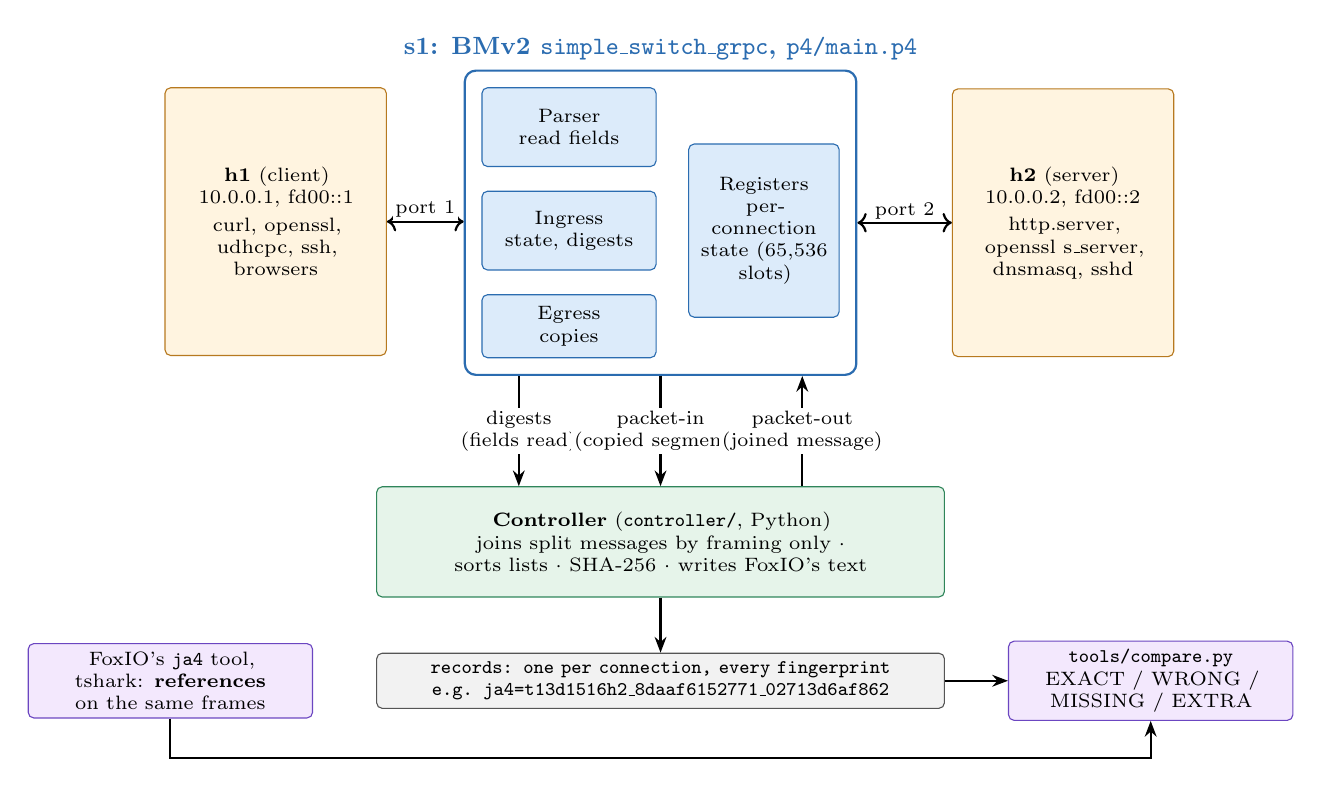
\begin{tikzpicture}[node distance=5mm and 6mm, every node/.style={font=\small}]
  % hosts
  \node[hobox, text width=26mm, minimum height=34mm] (h1) {\textbf{h1} (client)\\ 10.0.0.1, fd00::1\\[2pt]\scriptsize curl, openssl,\\ \scriptsize udhcpc, ssh,\\ \scriptsize browsers};
  % switch
  \node[swbox, right=12mm of h1, text width=20mm, minimum height=10mm, yshift=12mm] (par) {Parser\\ \scriptsize read fields};
  \node[swbox, below=3mm of par, text width=20mm, minimum height=10mm] (ing) {Ingress\\ \scriptsize state, digests};
  \node[swbox, below=3mm of ing, text width=20mm, minimum height=8mm] (eg) {Egress\\ \scriptsize copies};
  \node[swbox, right=4mm of ing, text width=17mm, minimum height=22mm] (reg) {Registers\\ \scriptsize per-connection\\ \scriptsize state (65,536\\ \scriptsize slots)};
  \node[grp, draw=swd, fit=(par)(ing)(eg)(reg), label={[font=\small\bfseries, text=swd]above:s1: BMv2 \code{simple\_switch\_grpc}, \code{p4/main.p4}}] (s1) {};
  % h2
  \node[hobox, right=12mm of s1, text width=26mm, minimum height=34mm] (h2) {\textbf{h2} (server)\\ 10.0.0.2, fd00::2\\[2pt]\scriptsize http.server,\\ \scriptsize openssl s\_server,\\ \scriptsize dnsmasq, sshd};
  \draw[arr, <->] (h1) -- node[lbl, above]{port 1} (h1 -| s1.west);
  \draw[arr, <->] (s1.east |- h2) -- node[lbl, above]{port 2} (h2);
  % controller
  \node[ctbox, below=14mm of s1, text width=70mm, minimum height=14mm] (ctl) {\textbf{Controller} (\code{controller/}, Python)\\ \scriptsize joins split messages by framing only $\cdot$ sorts lists $\cdot$ SHA-256 $\cdot$ writes FoxIO's text};
  \draw[arr] ($(s1.south)+(-18mm,0)$) -- node[lbl]{digests\\(fields read)} ($(ctl.north)+(-18mm,0)$);
  \draw[arr] ($(s1.south)+(0,0)$) -- node[lbl]{packet-in\\(copied segments)} ($(ctl.north)+(0,0)$);
  \draw[arr] ($(ctl.north)+(18mm,0)$) -- node[lbl]{packet-out\\(joined message)} ($(s1.south)+(18mm,0)$);
  % outputs
  \node[fibox, below=7mm of ctl, text width=70mm] (out) {records: one per connection, every fingerprint\\ e.g. ja4=t13d1516h2\_8daaf6152771\_02713d6af862};
  \draw[arr] (ctl) -- (out);
  % verification
  \node[rfbox, left=8mm of out, text width=34mm] (ref) {FoxIO's \code{ja4} tool,\\ tshark: \textbf{references}\\ \scriptsize on the same frames};
  \node[rfbox, right=8mm of out, text width=34mm] (cmp) {\code{tools/compare.py}\\ EXACT / WRONG /\\ MISSING / EXTRA};
  \draw[arr] (out) -- (cmp); \draw[arr] (ref.south) |- ++(0,-5mm) -| (cmp.south);
\end{tikzpicture}
\caption{The whole system. Every packet is forwarded unchanged between the hosts; the switch reads the clear-text
exchange and reports what it read; the controller only orders bytes and writes text; independent tools check the
result.}
\label{fig:glance}
\end{figure}

\subsection{Who does what, and why the line is drawn there}

\begin{figure}[H]\centering
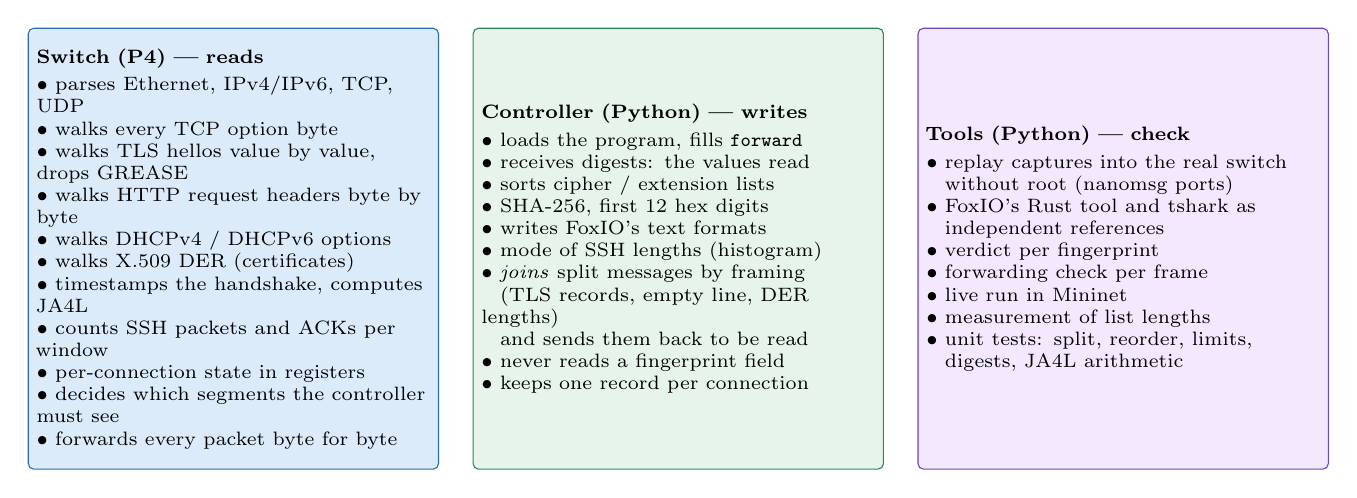
\begin{tikzpicture}[node distance=4mm]
  \node[swbox, text width=50mm, align=left, minimum height=56mm, anchor=north west] (s) at (0,0) {\textbf{Switch (P4) --- reads}\\[2pt]\scriptsize
  $\bullet$ parses Ethernet, IPv4/IPv6, TCP, UDP\\
  $\bullet$ walks every TCP option byte\\
  $\bullet$ walks TLS hellos value by value, drops GREASE\\
  $\bullet$ walks HTTP request headers byte by byte\\
  $\bullet$ walks DHCPv4 / DHCPv6 options\\
  $\bullet$ walks X.509 DER (certificates)\\
  $\bullet$ timestamps the handshake, computes JA4L\\
  $\bullet$ counts SSH packets and ACKs per window\\
  $\bullet$ per-connection state in registers\\
  $\bullet$ decides which segments the controller must see\\
  $\bullet$ forwards every packet byte for byte};
  \node[ctbox, text width=50mm, align=left, minimum height=56mm, anchor=north west] (c) at (5.65,0) {\textbf{Controller (Python) --- writes}\\[2pt]\scriptsize
  $\bullet$ loads the program, fills \code{forward}\\
  $\bullet$ receives digests: the values read\\
  $\bullet$ sorts cipher / extension lists\\
  $\bullet$ SHA-256, first 12 hex digits\\
  $\bullet$ writes FoxIO's text formats\\
  $\bullet$ mode of SSH lengths (histogram)\\
  $\bullet$ \emph{joins} split messages by framing\\
  \hphantom{$\bullet$} (TLS records, empty line, DER lengths)\\
  \hphantom{$\bullet$} and sends them back to be read\\
  $\bullet$ never reads a fingerprint field\\
  $\bullet$ keeps one record per connection};
  \node[rfbox, text width=50mm, align=left, minimum height=56mm, anchor=north west] (t) at (11.3,0) {\textbf{Tools (Python) --- check}\\[2pt]\scriptsize
  $\bullet$ replay captures into the real switch\\
  \hphantom{$\bullet$} without root (nanomsg ports)\\
  $\bullet$ FoxIO's Rust tool and tshark as\\
  \hphantom{$\bullet$} independent references\\
  $\bullet$ verdict per fingerprint\\
  $\bullet$ forwarding check per frame\\
  $\bullet$ live run in Mininet\\
  $\bullet$ measurement of list lengths\\
  $\bullet$ unit tests: split, reorder, limits,\\
  \hphantom{$\bullet$} digests, JA4L arithmetic};
\end{tikzpicture}
\caption{The division of work. The line: everything that must look at packet bytes to extract a fingerprint
value is in P4; what P4 on this target cannot do (sort, SHA-256, a histogram, text) is in the controller, working
only on values the switch extracted.}
\end{figure}

\why{The project's claim is ``fingerprinting done in P4''. Reading the clear-text exchange (the variable-length
parsing, GREASE, completeness, per-connection state, timing) is the hard part and is done in the data plane. The
v1model / BMv2 target has no SHA-256 extern, no loops outside the parser, no sorting, and no strings; those last
steps are cheap, need no packet bytes, and are done by the controller on the switch's output.}

\whynot{(1) The controller could parse whole packets sent to it (packet-in of every packet): that would be a
software fingerprinter with a switch in front, not P4 fingerprinting. (2) Sorting and hashing in P4: possible only
with a sorting network sized to the list (many pipeline stages on hardware) and a hash the target does not have;
the result would be identical and the claim no stronger. (3) No controller at all: the switch would have nowhere
to put the text, and split messages could not be joined (a P4 switch cannot hold packets back).}

%---------------------------------------------------------------------
\subsection{Map of the code: every file, what it feeds}
\label{sec:map}

\begin{figure}[H]\centering
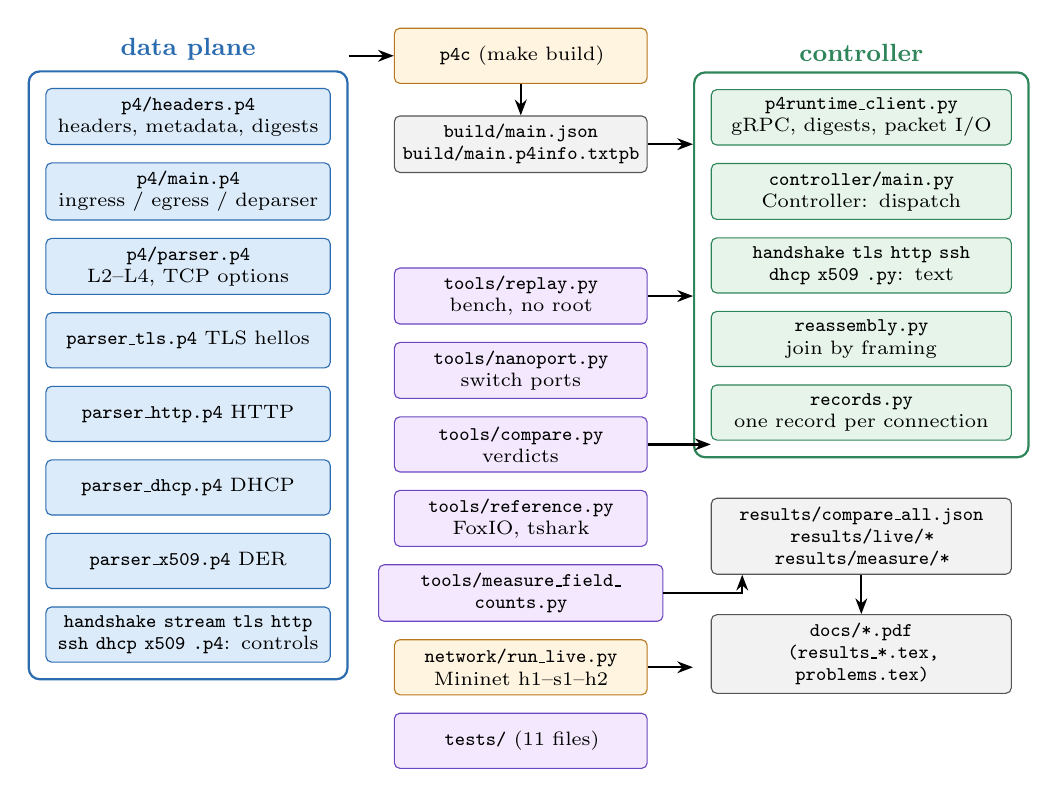
\begin{tikzpicture}[node distance=2.2mm, every node/.style={font=\scriptsize}]
  % P4 column
  \node[swbox, text width=34mm, font=\scriptsize] (main) {\code{p4/main.p4}\\ ingress / egress / deparser};
  \node[swbox, text width=34mm, font=\scriptsize, above=of main] (hdr) {\code{p4/headers.p4}\\ headers, metadata, digests};
  \node[swbox, text width=34mm, font=\scriptsize, below=of main] (par) {\code{p4/parser.p4}\\ L2--L4, TCP options};
  \node[swbox, text width=34mm, font=\scriptsize, below=of par] (ptls) {\code{parser\_tls.p4} TLS hellos};
  \node[swbox, text width=34mm, font=\scriptsize, below=of ptls] (phttp) {\code{parser\_http.p4} HTTP};
  \node[swbox, text width=34mm, font=\scriptsize, below=of phttp] (pdhcp) {\code{parser\_dhcp.p4} DHCP};
  \node[swbox, text width=34mm, font=\scriptsize, below=of pdhcp] (px509) {\code{parser\_x509.p4} DER};
  \node[swbox, text width=34mm, font=\scriptsize, below=of px509] (ctrls) {\code{handshake stream tls http}\\ \code{ssh dhcp x509 .p4}: controls};
  \node[grp, draw=swd, fit=(hdr)(ctrls), label={[text=swd, font=\small\bfseries]above:data plane}] (gp4) {};
  % build
  \node[fibox, right=8mm of main, text width=30mm, yshift=6mm] (json) {build/main.json\\ build/main.p4info.txtpb};
  \node[hobox, above=4mm of json, text width=30mm] (p4c) {\code{p4c} (make build)};
  \draw[arr] (gp4.east |- p4c) -- (p4c); \draw[arr] (p4c) -- (json);
  % controller column
  \node[ctbox, right=8mm of json, text width=36mm, font=\scriptsize, yshift=-6mm] (cmain) {\code{controller/main.py}\\ Controller: dispatch};
  \node[ctbox, above=of cmain, text width=36mm, font=\scriptsize] (client) {\code{p4runtime\_client.py}\\ gRPC, digests, packet I/O};
  \node[ctbox, below=of cmain, text width=36mm, font=\scriptsize] (fmt) {\code{handshake tls http ssh}\\ \code{dhcp x509 .py}: text};
  \node[ctbox, below=of fmt, text width=36mm, font=\scriptsize] (reasm) {\code{reassembly.py}\\ join by framing};
  \node[ctbox, below=of reasm, text width=36mm, font=\scriptsize] (recs) {\code{records.py}\\ one record per connection};
  \node[grp, draw=ctd, fit=(client)(recs), label={[text=ctd, font=\small\bfseries]above:controller}] (gct) {};
  \draw[arr] (json) -- (json -| gct.west);
  % tools
  \node[rfbox, below=12mm of json, text width=30mm, font=\scriptsize] (replay) {\code{tools/replay.py}\\ bench, no root};
  \node[rfbox, below=of replay, text width=30mm, font=\scriptsize] (nano) {\code{tools/nanoport.py}\\ switch ports};
  \node[rfbox, below=of nano, text width=30mm, font=\scriptsize] (cmp) {\code{tools/compare.py}\\ verdicts};
  \node[rfbox, below=of cmp, text width=30mm, font=\scriptsize] (ref) {\code{tools/reference.py}\\ FoxIO, tshark};
  \node[rfbox, below=of ref, text width=34mm, font=\scriptsize] (meas) {\code{tools/measure\_field\_}\\ \code{counts.py}};
  \node[hobox, below=of meas, text width=30mm, font=\scriptsize] (live) {\code{network/run\_live.py}\\ Mininet h1--s1--h2};
  \node[rfbox, below=of live, text width=30mm, font=\scriptsize] (tests) {\code{tests/} (11 files)};
  \draw[arr] (replay) -- (replay -| gct.west);
  \draw[arr] (live.east) -- (live -| gct.west);
  % results
  \node[fibox, below=5mm of gct, text width=36mm] (res) {results/compare\_all.json\\ results/live/*\\ results/measure/*};
  \draw[arr] (cmp.east) -- (cmp -| res.west) ; \draw[arr] (meas.east) -| ($(res.south west)+(4mm,0)$);
  \node[fibox, below=5mm of res, text width=36mm] (pdf) {docs/*.pdf\\ (results\_*.tex, problems.tex)};
  \draw[arr] (res) -- (pdf);
\end{tikzpicture}
\caption{Every code file and what it feeds. \code{make build} compiles the P4 files into the program the switch
runs; the controller loads it and talks to the switch; the tools drive switch + controller (replay without root, or
the live Mininet network), compare with the references and write results, which the PDFs include.}
\label{fig:map}
\end{figure}

%---------------------------------------------------------------------
\subsection{Build and run: what each command produces}

\begin{figure}[H]\centering
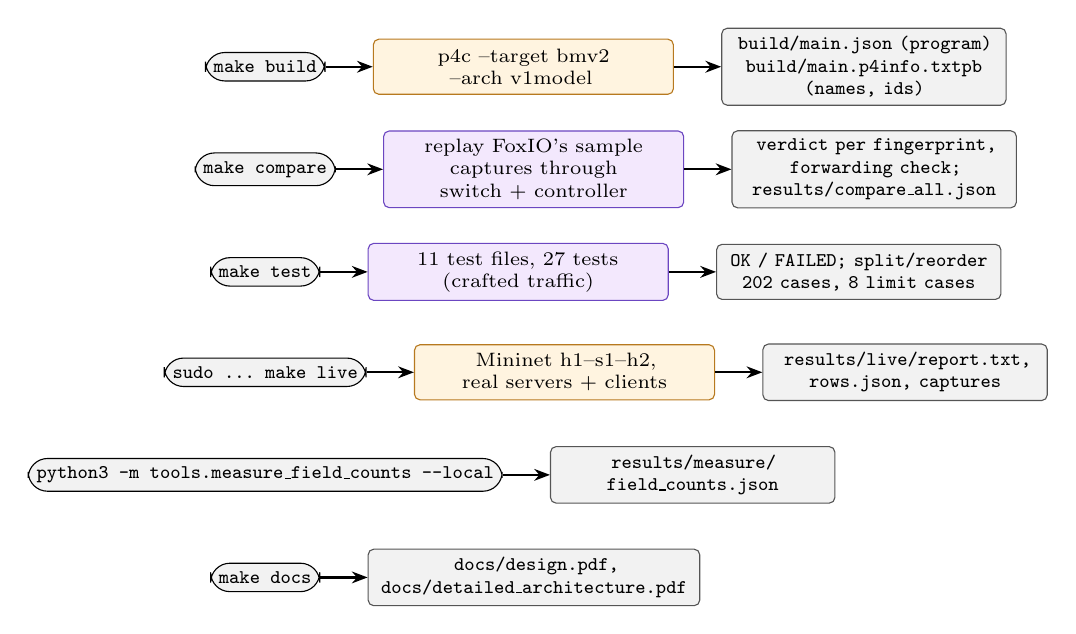
\begin{tikzpicture}[node distance=4mm and 6mm, every node/.style={font=\scriptsize}]
  \node[term] (b) {\code{make build}};
  \node[hobox, right=of b, text width=36mm, font=\scriptsize] (p4c) {p4c --target bmv2\\ --arch v1model};
  \node[fibox, right=of p4c, text width=34mm] (j) {build/main.json (program)\\ build/main.p4info.txtpb (names, ids)};
  \draw[arr] (b) -- (p4c); \draw[arr] (p4c) -- (j);
  \node[term, below=9mm of b] (c) {\code{make compare}};
  \node[rfbox, right=of c, text width=36mm, font=\scriptsize] (c1) {replay FoxIO's sample\\ captures through\\ switch + controller};
  \node[fibox, right=of c1, text width=34mm] (c2) {verdict per fingerprint,\\ forwarding check;\\ results/compare\_all.json};
  \draw[arr] (c) -- (c1); \draw[arr] (c1) -- (c2);
  \node[term, below=9mm of c] (t) {\code{make test}};
  \node[rfbox, right=of t, text width=36mm, font=\scriptsize] (t1) {11 test files, 27 tests\\ (crafted traffic)};
  \node[fibox, right=of t1, text width=34mm] (t2) {OK / FAILED; split/reorder\\ 202 cases, 8 limit cases};
  \draw[arr] (t) -- (t1); \draw[arr] (t1) -- (t2);
  \node[term, below=9mm of t] (l) {\code{sudo \ldots\ make live}};
  \node[hobox, right=of l, text width=36mm, font=\scriptsize] (l1) {Mininet h1--s1--h2,\\ real servers + clients};
  \node[fibox, right=of l1, text width=34mm] (l2) {results/live/report.txt,\\ rows.json, captures};
  \draw[arr] (l) -- (l1); \draw[arr] (l1) -- (l2);
  \node[term, below=9mm of l] (m) {\code{python3 -m tools.measure\_field\_counts --local}};
  \node[fibox, right=of m, text width=34mm, xshift=0mm] (m2) {results/measure/\\ field\_counts.json};
  \draw[arr] (m) -- (m2);
  \node[term, below=9mm of m] (d) {\code{make docs}};
  \node[fibox, right=of d, text width=40mm] (d2) {docs/design.pdf,\\ docs/detailed\_architecture.pdf};
  \draw[arr] (d) -- (d2);
\end{tikzpicture}
\caption{Commands and their outputs. Only \code{make live} needs root (Mininet's network namespaces).}
\end{figure}

%=====================================================================
\section{Inside the switch}
\label{sec:switch}

\subsection{Life of a packet through the pipeline}

\begin{figure}[H]\centering
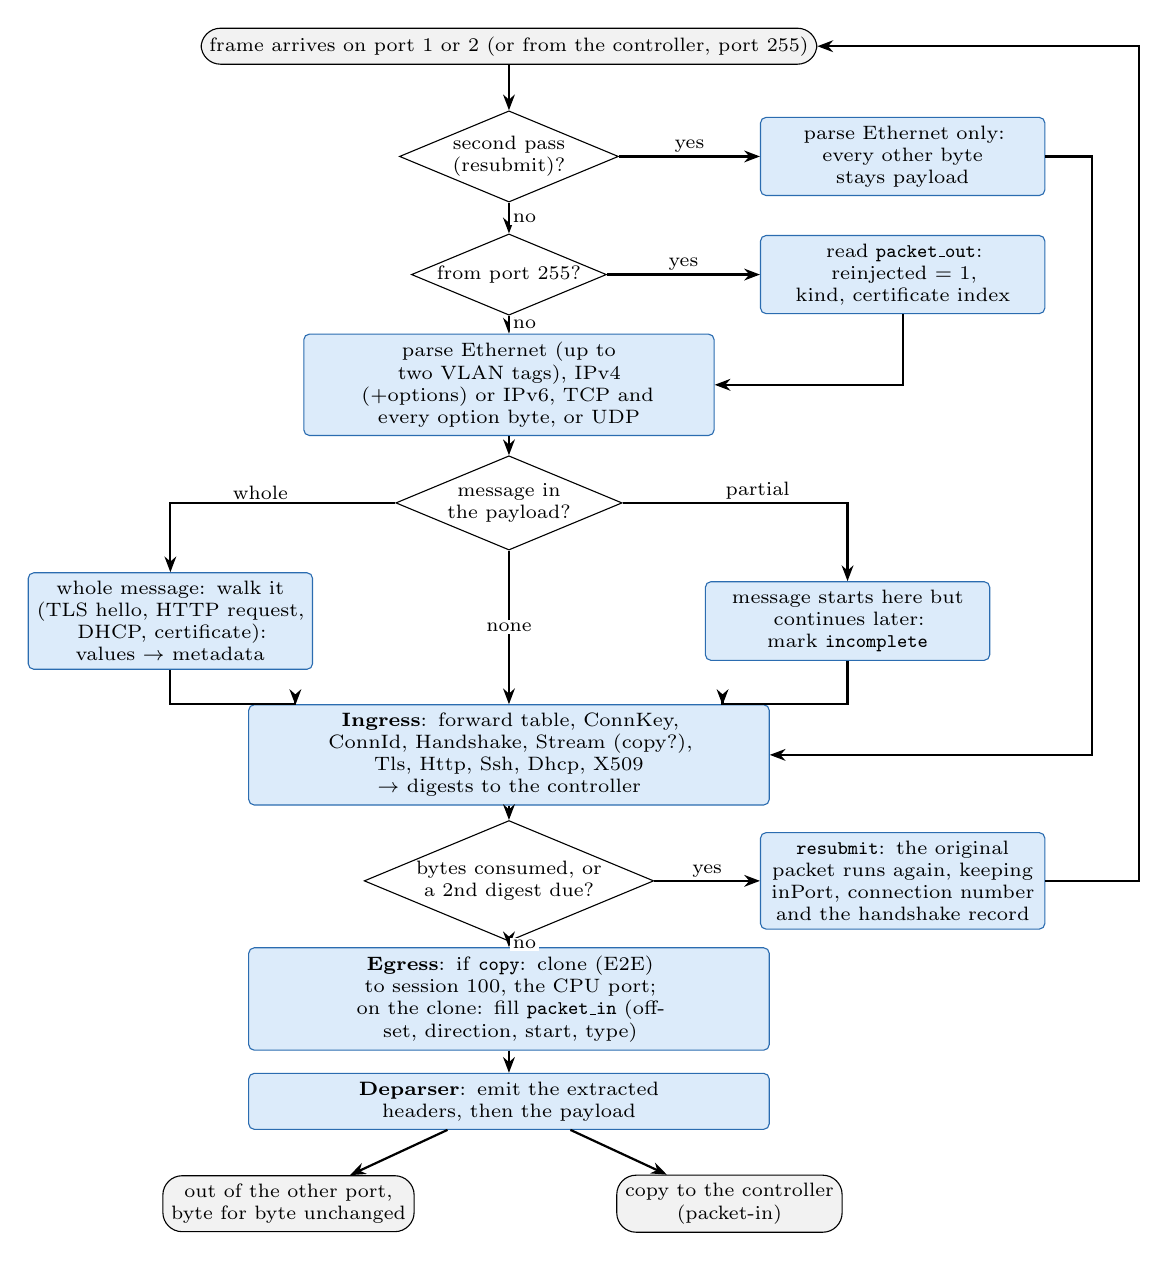
\begin{tikzpicture}
  \node[term] (in) at (0,0) {frame arrives on port 1 or 2 (or from the controller, port 255)};
  \node[dec] (inst) at (0,-1.4) {second pass\\ (resubmit)?};
  \node[swbox, text width=34mm] (eth) at (5,-1.4) {parse Ethernet only:\\ every other byte stays payload};
  \node[dec] (cpu) at (0,-2.9) {from port 255?};
  \node[swbox, text width=34mm] (po) at (5,-2.9) {read \code{packet\_out}: reinjected = 1,\\ kind, certificate index};
  \node[swbox, text width=50mm] (l34) at (0,-4.3) {parse Ethernet (up to two VLAN tags), IPv4\\ (+options) or IPv6, TCP and every option byte, or UDP};
  \node[dec] (pay) at (0,-5.8) {message in\\ the payload?};
  \node[swbox, text width=34mm] (walk) at (-4.3,-7.3) {whole message: walk it\\ (TLS hello, HTTP request,\\ DHCP, certificate):\\ values $\to$ metadata};
  \node[swbox, text width=34mm] (inc) at (4.3,-7.3) {message starts here but\\ continues later:\\ mark \code{incomplete}};
  \node[swbox, text width=64mm] (ing) at (0,-9.0) {\textbf{Ingress}: forward table, ConnKey, ConnId, Handshake, Stream (copy?),\\ Tls, Http, Ssh, Dhcp, X509 $\to$ digests to the controller};
  \node[dec] (wk) at (0,-10.6) {bytes consumed, or\\ a 2nd digest due?};
  \node[swbox, text width=34mm] (rs) at (5,-10.6) {\code{resubmit}: the original\\ packet runs again, keeping\\ inPort, connection number\\ and the handshake record};
  \node[swbox, text width=64mm] (eg) at (0,-12.1) {\textbf{Egress}: if \code{copy}: clone (E2E) to session 100, the CPU port;\\ on the clone: fill \code{packet\_in} (offset, direction, start, type)};
  \node[swbox, text width=64mm] (dp) at (0,-13.4) {\textbf{Deparser}: emit the extracted headers, then the payload};
  \node[term] (o1) at (-2.8,-14.7) {out of the other port,\\ byte for byte unchanged};
  \node[term] (o2) at (2.8,-14.7) {copy to the controller\\ (packet-in)};
  \draw[arr] (in) -- (inst);
  \draw[arr] (inst) -- node[lbl, above]{yes} (eth);
  \draw[arr] (inst) -- node[lbl, right]{no} (cpu);
  \draw[arr] (cpu) -- node[lbl, above]{yes} (po);
  \draw[arr] (po.south) |- ($(l34.east)+(0,0)$);
  \draw[arr] (cpu) -- node[lbl, right]{no} (l34);
  \draw[arr] (l34) -- (pay);
  \draw[arr] (pay) -| node[lbl, above, pos=0.3]{whole} (walk);
  \draw[arr] (pay) -| node[lbl, above, pos=0.3]{partial} (inc);
  \draw[arr] (pay) -- node[lbl]{none} (ing);
  \draw[arr] (walk) |- ($(ing.north west)+(6mm,0)$) -- ++(0,-0.01);
  \draw[arr] (inc) |- ($(ing.north east)+(-6mm,0)$) -- ++(0,-0.01);
  \draw[arr] (eth.east) -- (7.4,-1.4) |- ($(ing.east)+(0,0)$);
  \draw[arr] (ing) -- (wk);
  \draw[arr] (wk) -- node[lbl, above]{yes} (rs);
  \draw[arr] (rs.east) -- (8.0,-10.6) |- (in.east);
  \draw[arr] (wk) -- node[lbl, right]{no} (eg);
  \draw[arr] (eg) -- (dp); \draw[arr] (dp) -- (o1); \draw[arr] (dp) -- (o2);
\end{tikzpicture}
\caption{One packet's path (\code{p4/parser.p4}, \code{p4/main.p4}). A walk reads a message with \code{advance},
which removes the read bytes from the packet: such a packet is \emph{resubmitted}, and on the second pass only
Ethernet is parsed, so the original bytes are forwarded. A packet from the controller (port 255) is read the same
way but never forwarded.}
\label{fig:life}
\end{figure}

\why{\code{advance} is the only way for a v1model parser to skip bytes it does not extract; extracting every byte
into headers would need header stacks thousands of entries long and the deparser would have to re-emit all of
them. Skipping and forwarding the untouched original on a second pass keeps the walk cheap and the forwarding
exact (checked frame by frame: 9,013 of 9,013).}
\whynot{\emph{Clone first, then walk the clone:} an ingress clone is parsed again from the start, so it would
lose its bytes the same way. \emph{Recirculate:} goes through egress and the deparser, which would emit the already
shortened packet.}

%---------------------------------------------------------------------
\subsection{The parser: top-level state machine}

\begin{figure}[H]\centering
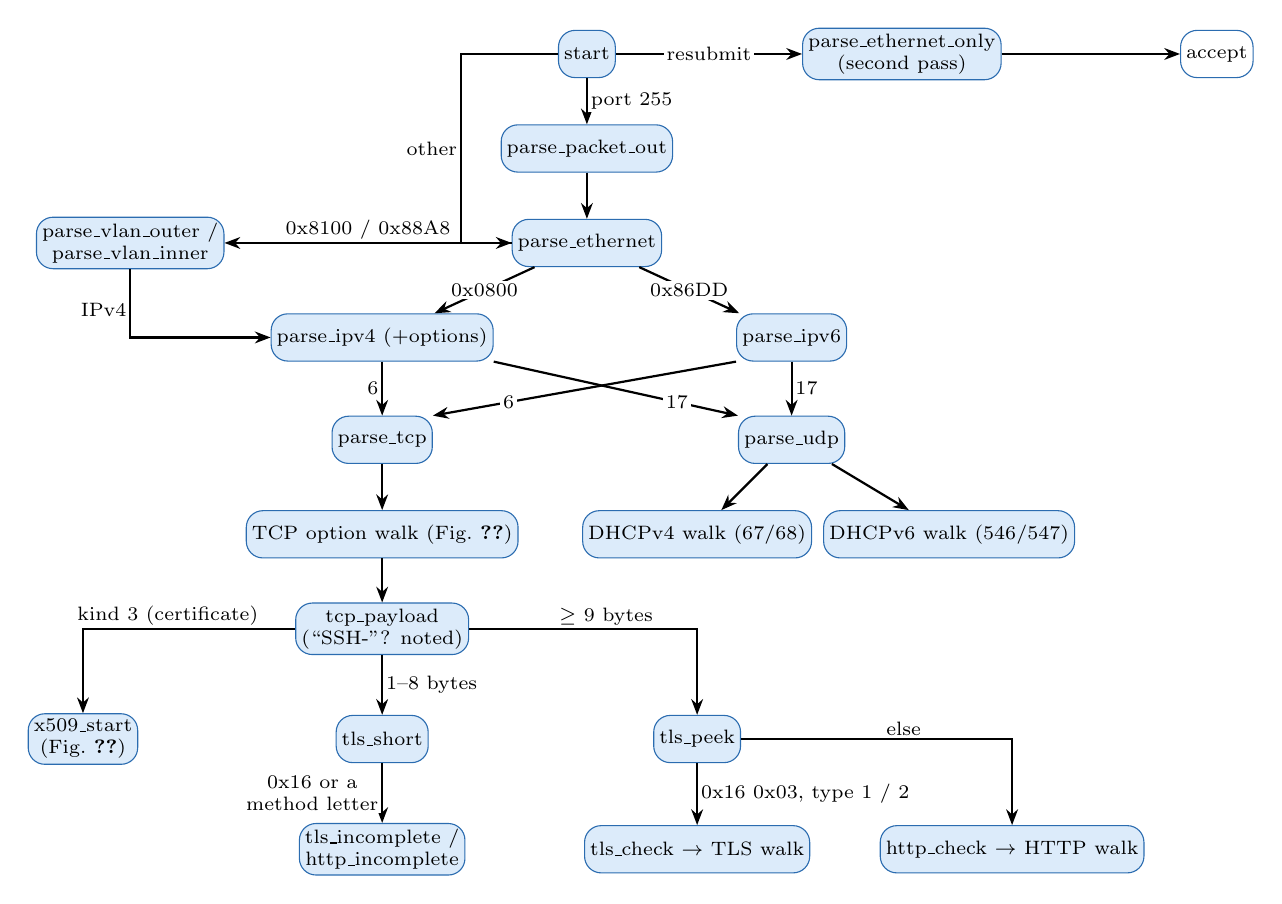
\begin{tikzpicture}
  \node[st] (start) at (0,0) {start};
  \node[st] (ethonly) at (4,0) {parse\_ethernet\_only\\ (second pass)};
  \node[st, fill=white] (acc) at (8,0) {accept};
  \node[st] (po) at (0,-1.2) {parse\_packet\_out};
  \node[st] (eth) at (0,-2.4) {parse\_ethernet};
  \node[st] (vl) at (-5.8,-2.4) {parse\_vlan\_outer /\\ parse\_vlan\_inner};
  \node[st] (v4) at (-2.6,-3.6) {parse\_ipv4 (+options)};
  \node[st] (v6) at (2.6,-3.6) {parse\_ipv6};
  \node[st] (tcp) at (-2.6,-4.9) {parse\_tcp};
  \node[st] (udp) at (2.6,-4.9) {parse\_udp};
  \node[st] (opt) at (-2.6,-6.1) {TCP option walk (Fig.~\ref{fig:opt})};
  \node[st] (d4) at (1.4,-6.1) {DHCPv4 walk (67/68)};
  \node[st] (d6) at (4.6,-6.1) {DHCPv6 walk (546/547)};
  \node[st] (tp) at (-2.6,-7.3) {tcp\_payload\\ (``SSH-''? noted)};
  \node[st] (x) at (-6.4,-8.7) {x509\_start\\ (Fig.~\ref{fig:x509})};
  \node[st] (short) at (-2.6,-8.7) {tls\_short};
  \node[st] (peek) at (1.4,-8.7) {tls\_peek};
  \node[st] (inc) at (-2.6,-10.1) {tls\_incomplete /\\ http\_incomplete};
  \node[st] (tlschk) at (1.4,-10.1) {tls\_check $\to$ TLS walk};
  \node[st] (httpchk) at (5.4,-10.1) {http\_check $\to$ HTTP walk};
  \draw[arr] (start) -- node[lbl]{resubmit} (ethonly);
  \draw[arr] (ethonly) -- (acc);
  \draw[arr] (start) -- node[lbl, right]{port 255} (po);
  \draw[arr] (start.west) -- (-1.6,0) |- node[lbl, pos=0.25, left]{other} (eth.west);
  \draw[arr] (po) -- (eth);
  \draw[arr] (eth) -- node[lbl]{0x0800} (v4); \draw[arr] (eth) -- node[lbl]{0x86DD} (v6);
  \draw[arr] (eth) -- node[lbl, above]{0x8100 / 0x88A8} (vl); \draw[arr] (vl) |- node[lbl, pos=0.3, left]{IPv4} (v4);
  \draw[arr] (v4) -- node[lbl, left]{6} (tcp); \draw[arr] (v6) -- node[lbl, right]{17} (udp);
  \draw[arr] (v4.south east) -- node[lbl, pos=0.75]{17} (udp.north west); \draw[arr] (v6.south west) -- node[lbl, pos=0.75]{6} (tcp.north east);
  \draw[arr] (tcp) -- (opt); \draw[arr] (opt) -- (tp);
  \draw[arr] (udp) -- (d4); \draw[arr] (udp) -- (d6);
  \draw[arr] (tp) -| node[lbl, pos=0.3, above]{kind 3 (certificate)} (x);
  \draw[arr] (tp) -- node[lbl, right]{1--8 bytes} (short);
  \draw[arr] (tp) -| node[lbl, pos=0.3, above]{$\ge$ 9 bytes} (peek);
  \draw[arr] (short) -- node[lbl, left]{0x16 or a\\ method letter} (inc);
  \draw[arr] (peek) -- node[lbl, right]{0x16 0x03, type 1 / 2} (tlschk);
  \draw[arr] (peek) -| node[lbl, pos=0.3, above]{else} (httpchk);
\end{tikzpicture}
\caption{The parser's top level (\code{parser.p4} with \code{parser\_tls.p4}, \code{parser\_http.p4},
\code{parser\_dhcp.p4}, \code{parser\_x509.p4} included inside it). IPv4 fragments other than the first are not
read beyond IP. Anything not matched goes to \code{accept}: the packet is still forwarded.}
\end{figure}

\begin{figure}[H]\centering
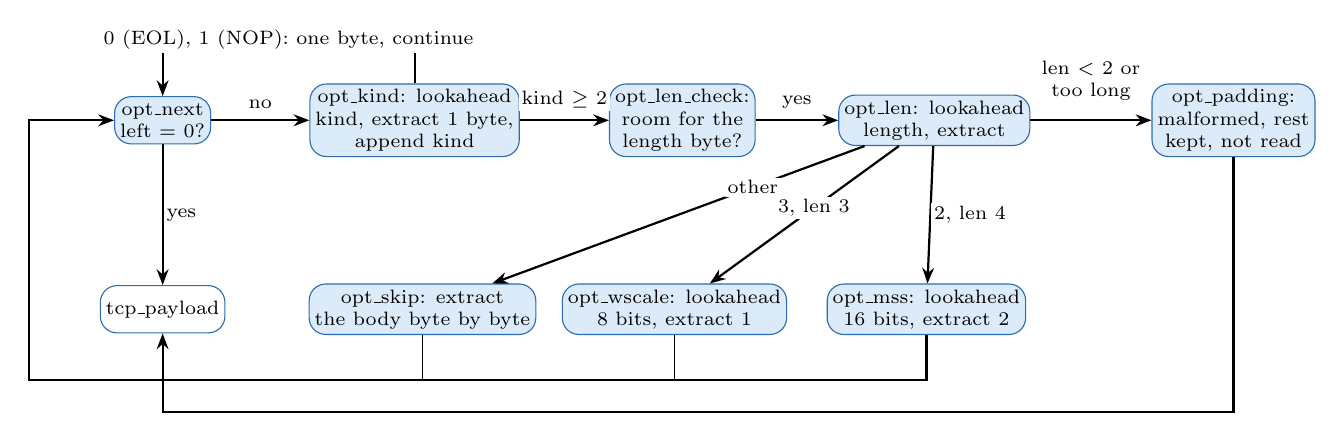
\begin{tikzpicture}
  \node[st] (next) at (0,0) {opt\_next\\ left = 0?};
  \node[st] (kind) at (3.2,0) {opt\_kind: lookahead\\ kind, extract 1 byte,\\ append kind};
  \node[st] (lc) at (6.6,0) {opt\_len\_check:\\ room for the\\ length byte?};
  \node[st] (len) at (9.8,0) {opt\_len: lookahead\\ length, extract};
  \node[st] (pad) at (13.6,0) {opt\_padding:\\ malformed, rest\\ kept, not read};
  \node[st, fill=white] (pay) at (0,-2.4) {tcp\_payload};
  \node[st] (skip) at (3.3,-2.4) {opt\_skip: extract\\ the body byte by byte};
  \node[st] (ws) at (6.5,-2.4) {opt\_wscale: lookahead\\ 8 bits, extract 1};
  \node[st] (mss) at (9.7,-2.4) {opt\_mss: lookahead\\ 16 bits, extract 2};
  \draw[arr] (next) -- node[lbl, above=1mm]{no} (kind);
  \draw[arr] (next) -- node[lbl, right]{yes} (pay);
  \draw[arr] (kind) -- node[lbl, above=1mm]{kind $\ge$ 2} (lc);
  \draw[arr] (kind.north) -- ++(0,0.55) -| node[lbl, pos=0.25]{0 (EOL), 1 (NOP): one byte, continue} (next.north);
  \draw[arr] (lc) -- node[lbl, above=1mm]{yes} (len);
  \draw[arr] (len) -- node[lbl, above=2mm]{len $<$ 2 or\\ too long} (pad);
  \draw[arr] (len) -- node[lbl, right]{2, len 4} (mss);
  \draw[arr] (len) -- node[lbl, pos=0.45]{3, len 3} (ws);
  \draw[arr] (len) -- node[lbl, pos=0.3]{other} (skip);
  \draw[arr] (pad.south) -- (13.6,-3.7) -| (pay.south);
  \draw[arr] (mss.south) -- (9.7,-3.3) -- (-1.7,-3.3) |- (next.west);
  \draw (ws.south) -- (6.5,-3.3); \draw (skip.south) -- (3.3,-3.3);
\end{tikzpicture}
\caption{TCP option walk (\code{parser.p4}): \code{left} = data offset $\times$ 4 $-$ 20 counts the option bytes
still to read, so the walk never reads payload. Every byte is \emph{extracted} (into \code{hdr.tcp\_opt}), so the
deparser re-emits the options unchanged and this walk needs no second pass. EOL is a one-byte option and the walk
continues: FoxIO (through tshark) lists every padding byte after EOL as another 0.}
\label{fig:opt}
\end{figure}

\begin{figure}[H]\centering
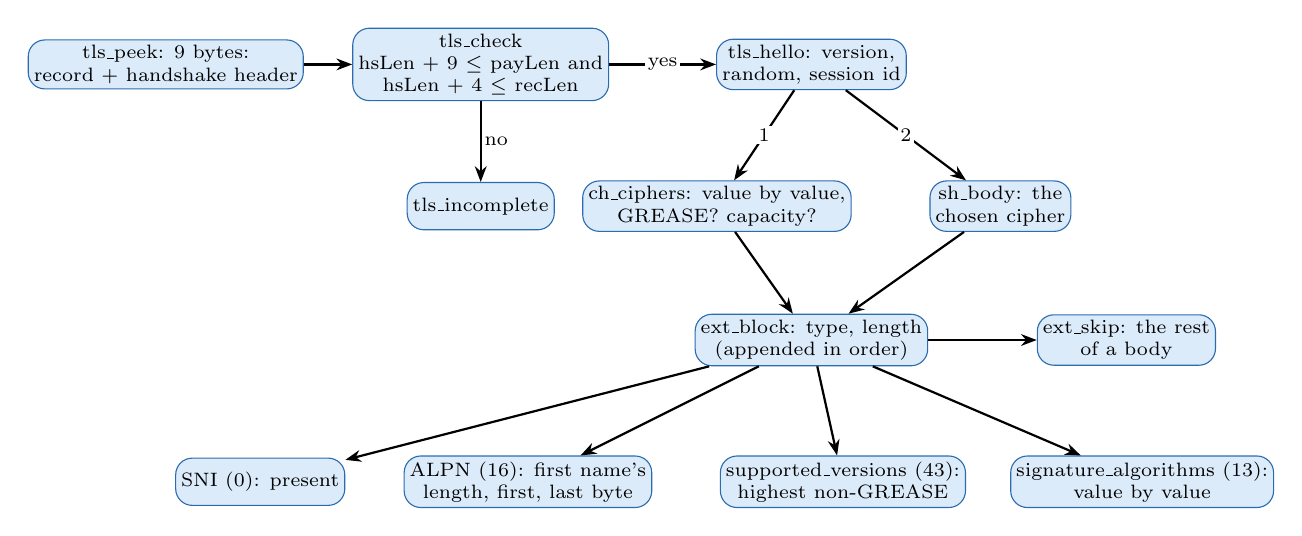
\begin{tikzpicture}
  \node[st] (peek) at (0,0) {tls\_peek: 9 bytes:\\ record + handshake header};
  \node[st] (chk) at (4.0,0) {tls\_check\\ hsLen + 9 $\le$ payLen and\\ hsLen + 4 $\le$ recLen};
  \node[st] (hello) at (8.2,0) {tls\_hello: version,\\ random, session id};
  \node[st] (inc) at (4.0,-1.8) {tls\_incomplete};
  \node[st] (ch) at (7.0,-1.8) {ch\_ciphers: value by value,\\ GREASE? capacity?};
  \node[st] (sh) at (10.6,-1.8) {sh\_body: the\\ chosen cipher};
  \node[st] (ext) at (8.2,-3.5) {ext\_block: type, length\\ (appended in order)};
  \node[st] (sk) at (12.2,-3.5) {ext\_skip: the rest\\ of a body};
  \node[st] (sni) at (1.2,-5.3) {SNI (0): present};
  \node[st] (alpn) at (4.6,-5.3) {ALPN (16): first name's\\ length, first, last byte};
  \node[st] (sv) at (8.6,-5.3) {supported\_versions (43):\\ highest non-GREASE};
  \node[st] (sig) at (12.4,-5.3) {signature\_algorithms (13):\\ value by value};
  \draw[arr] (peek) -- (chk); \draw[arr] (chk) -- node[lbl]{yes} (hello);
  \draw[arr] (chk) -- node[lbl, right]{no} (inc);
  \draw[arr] (hello) -- node[lbl]{1} (ch); \draw[arr] (hello) -- node[lbl]{2} (sh);
  \draw[arr] (ch) -- (ext); \draw[arr] (sh) -- (ext);
  \draw[arr] (ext) -- (sni); \draw[arr] (ext) -- (alpn); \draw[arr] (ext) -- (sv); \draw[arr] (ext) -- (sig);
  \draw[arr] (ext) -- (sk);
\end{tikzpicture}
\caption{TLS hello walk (\code{parser\_tls.p4}). Each list value is read with \code{lookahead} and skipped with
\code{advance}; a GREASE value (\code{0x?a?a}, equal bytes) goes back to the loop without being kept; a value
beyond the capacity sets an overflow bit. Every extension type is appended in order (client: without GREASE).}
\end{figure}

\begin{figure}[H]\centering
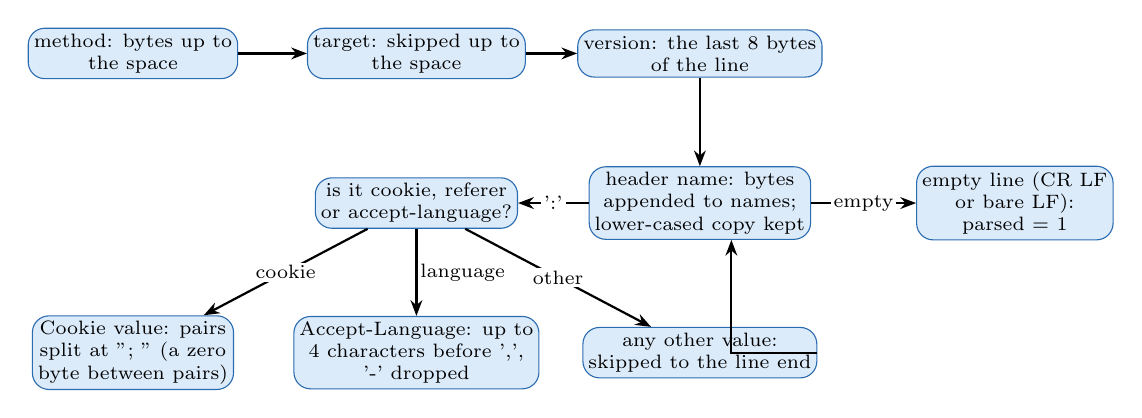
\begin{tikzpicture}
  \node[st] (m) at (0,0) {method: bytes up to\\ the space};
  \node[st] (t) at (3.6,0) {target: skipped up to\\ the space};
  \node[st] (v) at (7.2,0) {version: the last 8 bytes\\ of the line};
  \node[st] (n) at (7.2,-1.9) {header name: bytes\\ appended to names;\\ lower-cased copy kept};
  \node[st] (end) at (11.2,-1.9) {empty line (CR LF\\ or bare LF):\\ parsed = 1};
  \node[st] (k) at (3.6,-1.9) {is it cookie, referer\\ or accept-language?};
  \node[st] (cv) at (0,-3.8) {Cookie value: pairs\\ split at "; " (a zero\\ byte between pairs)};
  \node[st] (lv) at (3.6,-3.8) {Accept-Language: up to\\ 4 characters before ',',\\ '-' dropped};
  \node[st] (val) at (7.2,-3.8) {any other value:\\ skipped to the line end};
  \draw[arr] (m) -- (t); \draw[arr] (t) -- (v); \draw[arr] (v) -- (n); \draw[arr] (n) -- node[lbl]{':'} (k);
  \draw[arr] (k) -- node[lbl]{cookie} (cv); \draw[arr] (k) -- node[lbl, right]{language} (lv);
  \draw[arr] (k) -- node[lbl]{other} (val);
  \draw[arr] (n) -- node[lbl]{empty} (end);
  \draw[arr] (val.east) -| ($(n.south)+(4mm,0)$);
\end{tikzpicture}
\caption{HTTP request walk (\code{parser\_http.p4}), one byte per state. A name is appended to the names list as
it is read; when it turns out to be Cookie or Referer (excluded from JA4H's name list), the last 6 or 7 bytes are
removed with a constant-width slice. If the payload ends before the empty line, \code{incomplete} is set instead.}
\end{figure}

\begin{figure}[H]\centering
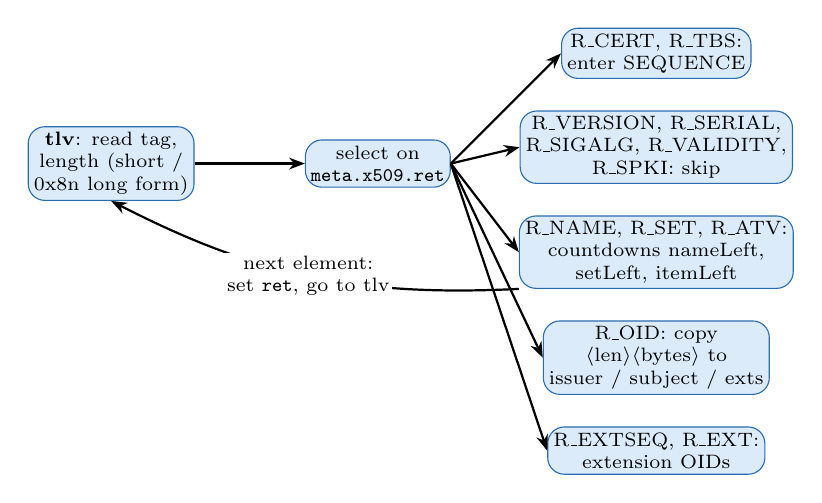
\begin{tikzpicture}[node distance=4mm and 5mm]
  \node[st] (tlv) {\textbf{tlv}: read tag,\\ length (short /\\ 0x8n long form)};
  \node[st, right=14mm of tlv] (ret) {select on\\ \code{meta.x509.ret}};
  \node[st, right=14mm of ret, yshift=14mm] (r1) {R\_CERT, R\_TBS:\\ enter SEQUENCE};
  \node[st, below=of r1] (r2) {R\_VERSION, R\_SERIAL,\\ R\_SIGALG, R\_VALIDITY,\\ R\_SPKI: skip};
  \node[st, below=of r2] (r3) {R\_NAME, R\_SET, R\_ATV:\\ countdowns nameLeft,\\ setLeft, itemLeft};
  \node[st, below=of r3] (r4) {R\_OID: copy\\ $\langle$len$\rangle\langle$bytes$\rangle$ to\\ issuer / subject / exts};
  \node[st, below=of r4] (r5) {R\_EXTSEQ, R\_EXT:\\ extension OIDs};
  \draw[arr] (tlv) -- (ret);
  \foreach \n in {r1,r2,r3,r4,r5} \draw[arr] (ret.east) -- (\n.west);
  \draw[arr] (r3.south west) to[bend left=15] node[lbl]{next element:\\ set \code{ret}, go to tlv} (tlv.south);
\end{tikzpicture}
\caption{DER walk (\code{parser\_x509.p4}). A P4 parser has no calls, so one shared \code{tlv} reader is entered
with a ``return code'' and a \code{select} on it continues in the right state. Nesting ends are known from byte
countdowns per level, so no stack is needed.}
\label{fig:x509}
\end{figure}

%---------------------------------------------------------------------
\subsection{Ingress: the order of the controls}

\begin{figure}[H]\centering
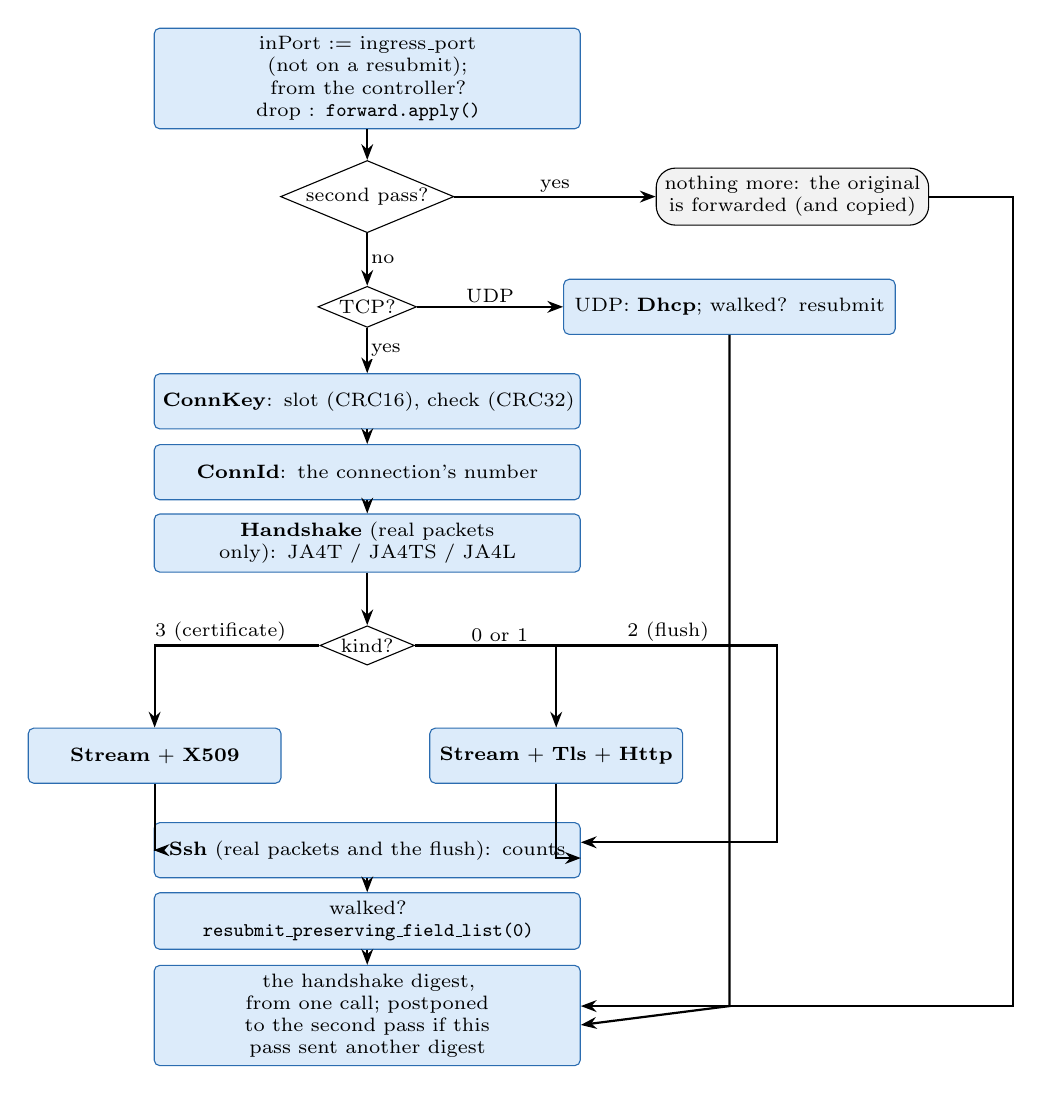
\begin{tikzpicture}
  \node[swbox, text width=52mm] (fw) at (0,0) {inPort := ingress\_port (not on a resubmit);\\ from the controller? drop : \code{forward.apply()}};
  \node[dec] (rs) at (0,-1.5) {second pass?};
  \node[term] (nothing) at (5.4,-1.5) {nothing more: the original\\ is forwarded (and copied)};
  \node[dec] (tcp) at (0,-2.9) {TCP?};
  \node[swbox, text width=40mm] (udp) at (4.6,-2.9) {UDP: \textbf{Dhcp}; walked? resubmit};
  \node[swbox, text width=52mm] (ck) at (0,-4.1) {\textbf{ConnKey}: slot (CRC16), check (CRC32)};
  \node[swbox, text width=52mm] (cid) at (0,-5.0) {\textbf{ConnId}: the connection's number};
  \node[swbox, text width=52mm] (hs) at (0,-5.9) {\textbf{Handshake} (real packets only): JA4T / JA4TS / JA4L};
  \node[dec] (k) at (0,-7.2) {kind?};
  \node[swbox, text width=30mm] (cert) at (-2.7,-8.6) {\textbf{Stream} + \textbf{X509}};
  \node[swbox, text width=30mm] (msg) at (2.4,-8.6) {\textbf{Stream} + \textbf{Tls} + \textbf{Http}};
  \node[swbox, text width=52mm] (ssh) at (0,-9.8) {\textbf{Ssh} (real packets and the flush): counts};
  \node[swbox, text width=52mm] (re) at (0,-10.7) {walked? \code{resubmit\_preserving\_field\_list(0)}};
  \node[swbox, text width=52mm] (hd) at (0,-11.9) {the handshake digest, from one call; postponed\\ to the second pass if this pass sent another digest};
  \draw[arr] (fw) -- (rs); \draw[arr] (rs) -- node[lbl, above]{yes} (nothing);
  \draw[arr] (rs) -- node[lbl, right]{no} (tcp); \draw[arr] (tcp) -- node[lbl, above]{UDP} (udp);
  \draw[arr] (tcp) -- node[lbl, right]{yes} (ck); \draw[arr] (ck) -- (cid); \draw[arr] (cid) -- (hs); \draw[arr] (hs) -- (k);
  \draw[arr] (k) -| node[lbl, above, pos=0.3]{3 (certificate)} (cert); \draw[arr] (k) -| node[lbl, above, pos=0.3]{0 or 1} (msg);
  \draw[arr] (k.east) -- node[lbl, above, pos=0.7]{2 (flush)} (5.2,-7.2) |- ($(ssh.east)+(0,0.1)$);
  \draw[arr] (cert) |- (ssh.west); \draw[arr] (msg) |- ($(ssh.east)+(0,-0.1)$);
  \draw[arr] (ssh) -- (re); \draw[arr] (re) -- (hd);
  \draw[arr] (nothing.east) -- (8.2,-1.5) |- ($(hd.east)+(0,0.12)$);
  \draw[arr] (udp.south) -- (4.6,-11.78) -- ($(hd.east)+(0,-0.12)$);
\end{tikzpicture}
\caption{\code{MyIngress} in \code{main.p4}. ``kind'' is the packet-out kind of a packet from the controller (0
for a real packet): 1 a joined message, 2 an SSH flush (Ssh only), 3 a certificate. Ssh runs after Stream, which
sets the packet's direction (client or server) that Ssh needs on ports other than 22.}
\end{figure}

\why{Every control is applied exactly once and in this order because (a) BMv2 allows a table / control instance
to be applied in one place only, (b) Stream must see the parse result (incomplete, parsed) before Tls/Http decide
to report, and (c) BMv2 keeps \emph{one digest per packet}: the handshake digest is therefore taken out of
Handshake and sent at the end, from one call, and postponed to the second pass when this pass sends a message
digest (the handshake's ACK can carry a whole ClientHello) or Ssh's digest (on the SYN of a reused port, the previous
connection's last window; on an SSH banner piggybacked on the handshake's ACK).}

%---------------------------------------------------------------------
\subsection{Per-connection state}

\begin{figure}[H]\centering
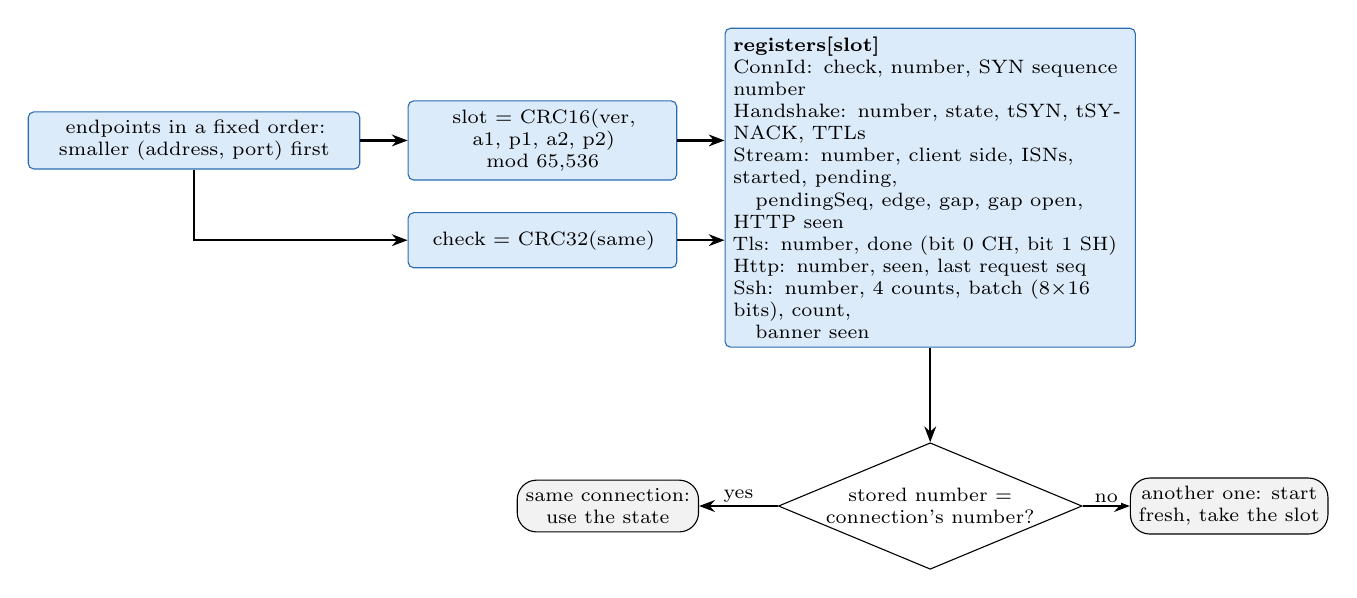
\begin{tikzpicture}[node distance=4mm and 6mm, every node/.style={font=\scriptsize}]
  \node[swbox, text width=40mm] (k) {endpoints in a fixed order:\\ smaller (address, port) first};
  \node[swbox, right=of k, text width=32mm] (h1) {slot = CRC16(ver, a1, p1, a2, p2)\\ mod 65,536};
  \node[swbox, below=of h1, text width=32mm] (h2) {check = CRC32(same)};
  \node[swbox, right=of h1, text width=50mm, yshift=-6mm, minimum height=26mm, align=left] (regs) {\textbf{registers[slot]}\\
    ConnId: check, number, SYN sequence number\\
    Handshake: number, state, tSYN, tSYNACK, TTLs\\
    Stream: number, client side, ISNs, started, pending,\\ \quad pendingSeq, edge, gap, gap open, HTTP seen\\
    Tls: number, done (bit 0 CH, bit 1 SH)\\
    Http: number, seen, last request seq\\
    Ssh: number, 4 counts, batch (8$\times$16 bits), count,\\ \quad banner seen};
  \draw[arr] (k) -- (h1); \draw[arr] (k) |- (h2);
  \draw[arr] (h1) -- (h1 -| regs.west); \draw[arr] (h2) -- (h2 -| regs.west);
  \node[dec, below=12mm of regs] (m) {stored number =\\ connection's number?};
  \node[term, left=10mm of m] (same) {same connection:\\ use the state};
  \node[term, right=6mm of m] (new) {another one: start\\ fresh, take the slot};
  \draw[arr] (regs) -- (m); \draw[arr] (m) -- node[lbl, above]{yes} (same); \draw[arr] (m) -- node[lbl, above]{no} (new);
\end{tikzpicture}
\caption{ConnKey and ConnId (\code{main.p4}) and the registers. Both directions of a connection find the same slot.
ConnId gives the connection a number: a new one when another connection (a different check) comes to the slot, and
when a SYN with a new initial sequence number arrives on the same endpoints (port reuse); a repeated SYN keeps it.
Every control keeps its state with this number, and every digest and copy carries it.}
\end{figure}

\why{A P4 switch cannot insert table entries itself, so per-connection state lives in register arrays indexed by a
hash. CRC16 gives the index; the independent CRC32 tells two connections in one slot apart with a 1 in $2^{32}$
chance of a false match.}
\why{\emph{The connection number}: the endpoints alone do not identify a connection. A client, and much faster a NAT,
reuses addresses and ports for a new connection after the old one closed. Before the number, the second
connection's fingerprints were dropped by the controller (it kept the first value per endpoints) and SSH counts of
the two connections were added together into a wrong JA4SSH (found by \code{test\_port\_reuse}).}
\whynot{\emph{The controller installs one table entry per connection:} each new connection would wait for a
round trip to the controller before its SYN state exists, and the SYN's timestamp (JA4L) would be lost.
\emph{A larger hash:} 65,536 slots is plenty for one link of a test network; the size is one constant.}

%=====================================================================
\section{Switch and controller: every channel between them}
\label{sec:channels}

\begin{figure}[H]\centering
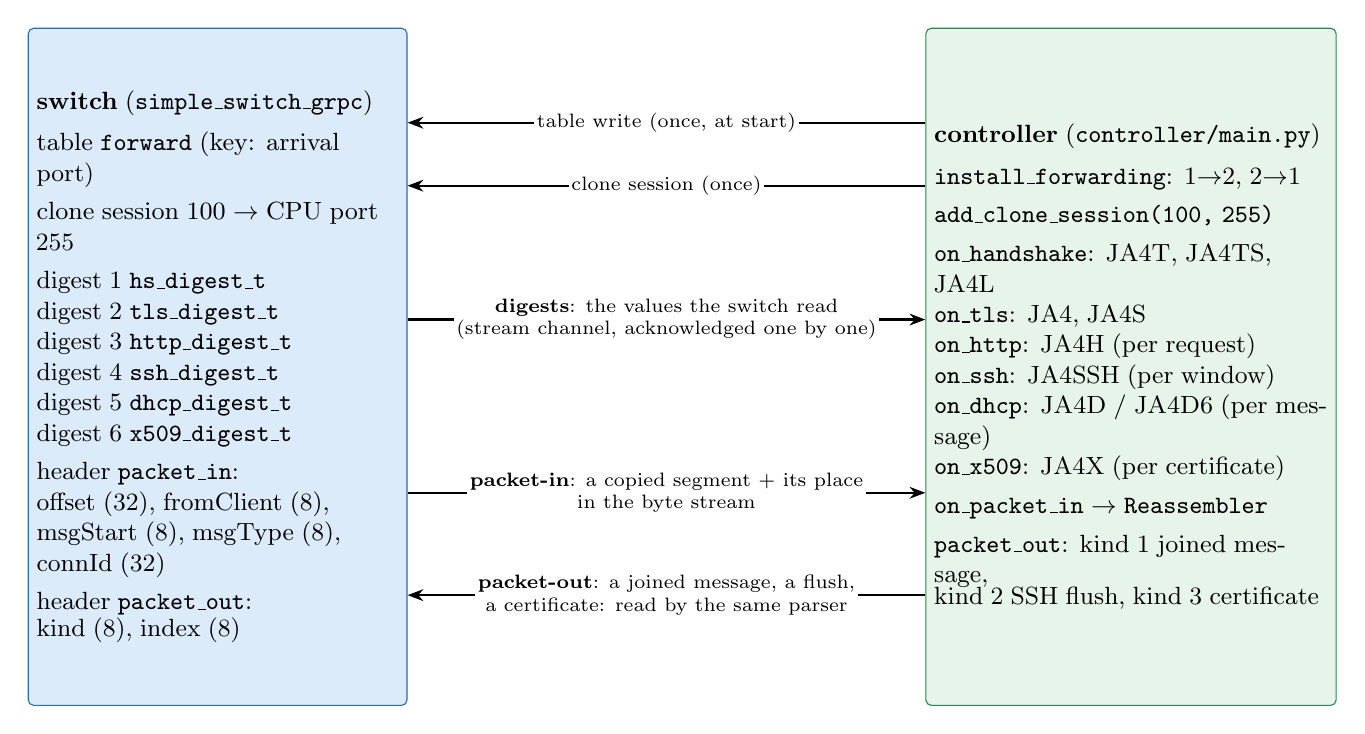
\begin{tikzpicture}
  \node[swbox, text width=46mm, minimum height=86mm, align=left] (s) at (0,0) {\small\textbf{switch} (\code{simple\_switch\_grpc})\\[4pt]
    table \code{forward} (key: arrival port)\\[3pt]
    clone session 100 $\to$ CPU port 255\\[3pt]
    digest 1 \code{hs\_digest\_t}\\
    digest 2 \code{tls\_digest\_t}\\
    digest 3 \code{http\_digest\_t}\\
    digest 4 \code{ssh\_digest\_t}\\
    digest 5 \code{dhcp\_digest\_t}\\
    digest 6 \code{x509\_digest\_t}\\[3pt]
    header \code{packet\_in}:\\ offset (32), fromClient (8),\\ msgStart (8), msgType (8),\\ connId (32)\\[3pt]
    header \code{packet\_out}:\\ kind (8), index (8)};
  \node[ctbox, text width=50mm, minimum height=86mm, align=left] (c) at (11.6,0) {\small\textbf{controller} (\code{controller/main.py})\\[4pt]
    \code{install\_forwarding}: 1$\to$2, 2$\to$1\\[3pt]
    \code{add\_clone\_session(100, 255)}\\[3pt]
    \code{on\_handshake}: JA4T, JA4TS, JA4L\\
    \code{on\_tls}: JA4, JA4S\\
    \code{on\_http}: JA4H (per request)\\
    \code{on\_ssh}: JA4SSH (per window)\\
    \code{on\_dhcp}: JA4D / JA4D6 (per message)\\
    \code{on\_x509}: JA4X (per certificate)\\[3pt]
    \code{on\_packet\_in} $\to$ \code{Reassembler}\\[3pt]
    \code{packet\_out}: kind 1 joined message,\\ kind 2 SSH flush, kind 3 certificate};
  \draw[arr] ($(c.west)+(0,3.1)$) -- node[lbl]{table write (once, at start)} ($(s.east)+(0,3.1)$);
  \draw[arr] ($(c.west)+(0,2.3)$) -- node[lbl]{clone session (once)} ($(s.east)+(0,2.3)$);
  \draw[arr] ($(s.east)+(0,0.6)$) -- node[lbl]{\textbf{digests}: the values the switch read\\ (stream channel, acknowledged one by one)} ($(c.west)+(0,0.6)$);
  \draw[arr] ($(s.east)+(0,-1.6)$) -- node[lbl]{\textbf{packet-in}: a copied segment + its place\\ in the byte stream} ($(c.west)+(0,-1.6)$);
  \draw[arr] ($(c.west)+(0,-2.9)$) -- node[lbl]{\textbf{packet-out}: a joined message, a flush,\\ a certificate: read by the same parser} ($(s.east)+(0,-2.9)$);
\end{tikzpicture}
\caption{The interface. Everything goes over one P4Runtime gRPC connection (\code{controller/p4runtime\_client.py}):
the controller becomes primary (arbitration), loads \code{build/main.json} with its P4Info, writes the table entries
and the clone session, enables the six digests, and then only listens and answers.}
\end{figure}

\subsection{The six digests}
\begin{center}\footnotesize
\begin{tabularx}{\textwidth}{c l >{\raggedright\arraybackslash}X >{\raggedright\arraybackslash}X >{\raggedright\arraybackslash}p{30mm}}
\toprule
\textbf{id} & \textbf{struct} & \textbf{sent when} & \textbf{main fields} & \textbf{controller writes} \\
\midrule
1 & \code{hs\_digest\_t} & first SYN (JA4T), first SYN-ACK (JA4TS), the ACK after it (JA4L) & window, option kinds (up to 40), MSS, window scale, two latencies, two TTLs, connId & \code{handshake.py}: \code{64240\_2-4-8-1-3\_1460\_7}, \code{1029\_64} \\
2 & \code{tls\_digest\_t} & a complete hello, once per connection and direction & versions, SNI flag, ciphers ($\le$128), extensions ($\le$64), signature algorithms ($\le$64), ALPN first/last, overflow, connId & \code{tls.py}: sort, SHA-256 $\to$ \code{t13d1516h2\_\ldots} \\
3 & \code{http\_digest\_t} & a complete request header block (not twice for one sequence number) & method, version, cookie / referer flags, header count, language, names ($\le$512 B), cookie pairs ($\le$1,024 B), serial, connId, the request's sequence number (the controller lists a connection's requests in stream order) & \code{http.py} $\to$ \code{ge11cr04engb\_\ldots} \\
4 & \code{ssh\_digest\_t} & 8 lengths collected; window of 200 closed; flush; an earlier connection's last window on a reused port's SYN; an SSH banner on a port other than 22 & batch of 8 (direction + length), 4 counts, serial, connId, direction & \code{ssh.py}: modes $\to$ \code{c36s52\_c100s100\_c0s0} \\
5 & \code{dhcp\_digest\_t} & every DHCP / DHCPv6 message & type, size, i/d flags, options ($\le$64), requested codes ($\le$128), serial & \code{dhcp.py} $\to$ \code{disco0576nn\_\ldots} \\
6 & \code{x509\_digest\_t} & every certificate sent back by the controller & chain index, issuer / subject / extension OIDs ($\le$256 B each), connId & \code{x509.py}: hex, SHA-256 $\to$ \code{a373a9f83c6b\_\ldots} \\
\bottomrule
\end{tabularx}
\end{center}

\textbf{Digest settings} (\code{enable\_digest}): \code{max\_list\_size = 1} and \code{max\_timeout\_ns = 0} (send
each digest at once, alone), \code{ack\_timeout\_ns} = 1\,s. The controller acknowledges every list as it handles
it. BMv2 holds an unacknowledged digest in a filter and drops an identical one: the DHCP, HTTP and SSH digests carry
a serial number for that reason (Section~\ref{sec:dec-serial}). Every digest of a TCP connection carries the
connection's number (\code{connId}, ConnId in \code{main.p4}): the controller keeps one record per (endpoints,
number), so a new connection on reused ports gets its own record.

%---------------------------------------------------------------------
\subsection{A message split over segments, arriving out of order}
\label{sec:seq}

\begin{figure}[H]\centering
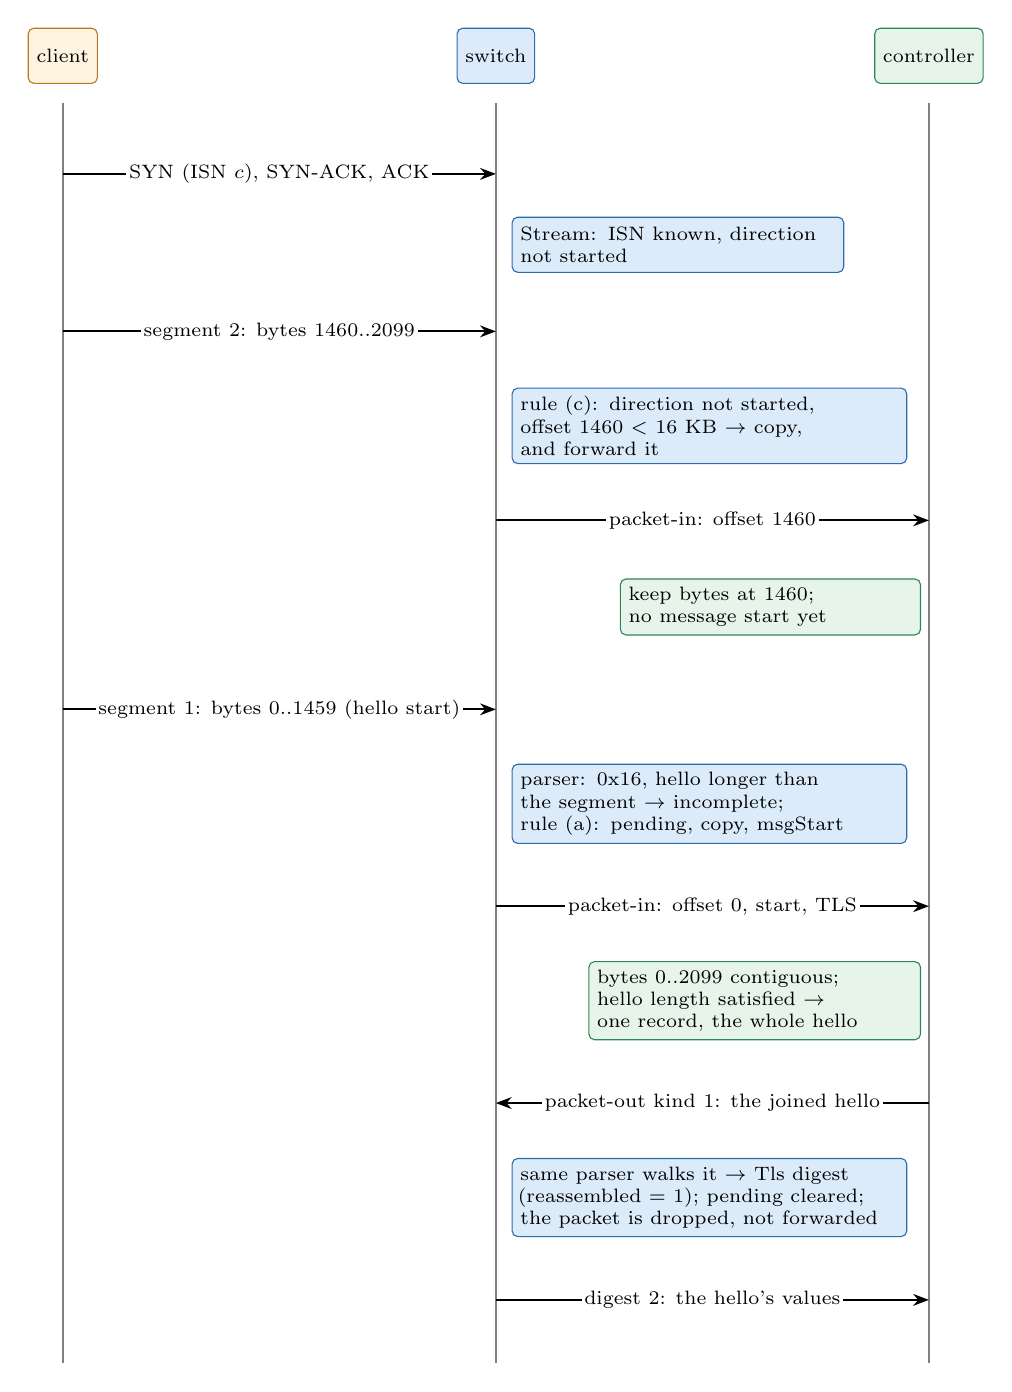
\begin{tikzpicture}[yscale=1.0]
  \node[hobox] (cl) at (0,0) {client};
  \node[swbox] (sw) at (5.5,0) {switch};
  \node[ctbox] (ct) at (11,0) {controller};
  \foreach \x in {0,5.5,11} \draw[thick, gray] (\x,-0.6) -- (\x,-16.6);
  \draw[arr] (0,-1.5) -- node[lbl]{SYN (ISN $c$), SYN-ACK, ACK} (5.5,-1.5);
  \node[swbox, right, text width=40mm, align=left] at (5.7,-2.4) {Stream: ISN known, direction not started};
  \draw[arr] (0,-3.5) -- node[lbl]{segment 2: bytes 1460..2099} (5.5,-3.5);
  \node[swbox, right, text width=48mm, align=left] at (5.7,-4.7) {rule (c): direction not started,\\ offset 1460 $<$ 16 KB $\to$ copy,\\ and forward it};
  \draw[arr] (5.5,-5.9) -- node[lbl]{packet-in: offset 1460} (11,-5.9);
  \node[ctbox, left, text width=36mm, align=left] at (10.9,-7.0) {keep bytes at 1460;\\ no message start yet};
  \draw[arr] (0,-8.3) -- node[lbl]{segment 1: bytes 0..1459 (hello start)} (5.5,-8.3);
  \node[swbox, right, text width=48mm, align=left] at (5.7,-9.5) {parser: 0x16, hello longer than\\ the segment $\to$ incomplete;\\ rule (a): pending, copy, msgStart};
  \draw[arr] (5.5,-10.8) -- node[lbl]{packet-in: offset 0, start, TLS} (11,-10.8);
  \node[ctbox, left, text width=40mm, align=left] at (10.9,-12.0) {bytes 0..2099 contiguous;\\ hello length satisfied $\to$\\ one record, the whole hello};
  \draw[arr] (11,-13.3) -- node[lbl]{packet-out kind 1: the joined hello} (5.5,-13.3);
  \node[swbox, right, text width=48mm, align=left] at (5.7,-14.5) {same parser walks it $\to$ Tls digest\\ (reassembled = 1); pending cleared;\\ the packet is dropped, not forwarded};
  \draw[arr] (5.5,-15.8) -- node[lbl]{digest 2: the hello's values} (11,-15.8);
\end{tikzpicture}
\caption{The out-of-order case end to end. The original segments are forwarded unchanged as they pass; only copies
go to the controller. The controller joins bytes by TLS framing only and never reads a field: the fingerprint is
still read by the switch's parser.}
\end{figure}

\begin{figure}[H]\centering
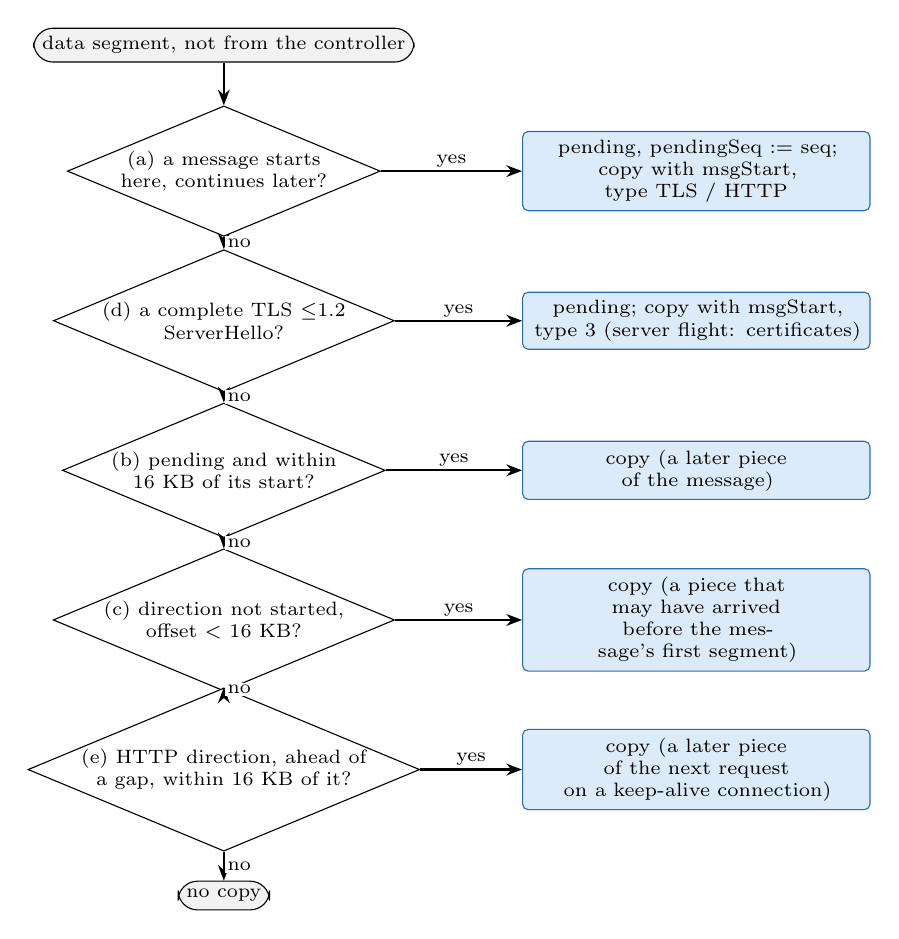
\begin{tikzpicture}
  \node[term] (s) at (0,0) {data segment, not from the controller};
  \node[dec] (a) at (0,-1.6) {(a) a message starts\\ here, continues later?};
  \node[swbox, text width=42mm] (ay) at (6.0,-1.6) {pending, pendingSeq := seq;\\ copy with msgStart, type TLS / HTTP};
  \node[dec] (d) at (0,-3.5) {(d) a complete TLS $\le$1.2\\ ServerHello?};
  \node[swbox, text width=42mm] (dy) at (6.0,-3.5) {pending; copy with msgStart,\\ type 3 (server flight: certificates)};
  \node[dec] (b) at (0,-5.4) {(b) pending and within\\ 16 KB of its start?};
  \node[swbox, text width=42mm] (by) at (6.0,-5.4) {copy (a later piece of the message)};
  \node[dec] (c) at (0,-7.3) {(c) direction not started,\\ offset $<$ 16 KB?};
  \node[swbox, text width=42mm] (cy) at (6.0,-7.3) {copy (a piece that may have arrived\\ before the message's first segment)};
  \node[dec] (e) at (0,-9.2) {(e) HTTP direction, ahead of\\ a gap, within 16 KB of it?};
  \node[swbox, text width=42mm] (ey) at (6.0,-9.2) {copy (a later piece of the next request\\ on a keep-alive connection)};
  \node[term] (no) at (0,-10.8) {no copy};
  \draw[arr] (s) -- (a); \draw[arr] (a) -- node[lbl, above]{yes} (ay);
  \draw[arr] (a) -- node[lbl, right]{no} (d); \draw[arr] (d) -- node[lbl, above]{yes} (dy);
  \draw[arr] (d) -- node[lbl, right]{no} (b); \draw[arr] (b) -- node[lbl, above]{yes} (by);
  \draw[arr] (b) -- node[lbl, right]{no} (c); \draw[arr] (c) -- node[lbl, above]{yes} (cy);
  \draw[arr] (c) -- node[lbl, right]{no} (e); \draw[arr] (e) -- node[lbl, above]{yes} (ey);
  \draw[arr] (e) -- node[lbl, right]{no} (no);
\end{tikzpicture}
\caption{\code{p4/stream.p4}: which segments the controller must see. Offsets are \code{seq} $-$ ISN $-$ 1 per
direction (ISN from the SYN / SYN-ACK; without them, learned from the first message start). A joined message (or
the certificates) coming back clears \code{pending}. For (e) the switch keeps, per direction, the \emph{edge} (the
sequence number after the furthest byte seen): a segment beyond it opens a gap at the edge; the gap closes when a
segment covering its first byte arrives, and is given up 16 KB on. Everything else is forwarded without a copy: the
controller sees only what a split message may need.}
\label{fig:copyrules}
\end{figure}

\begin{figure}[H]\centering
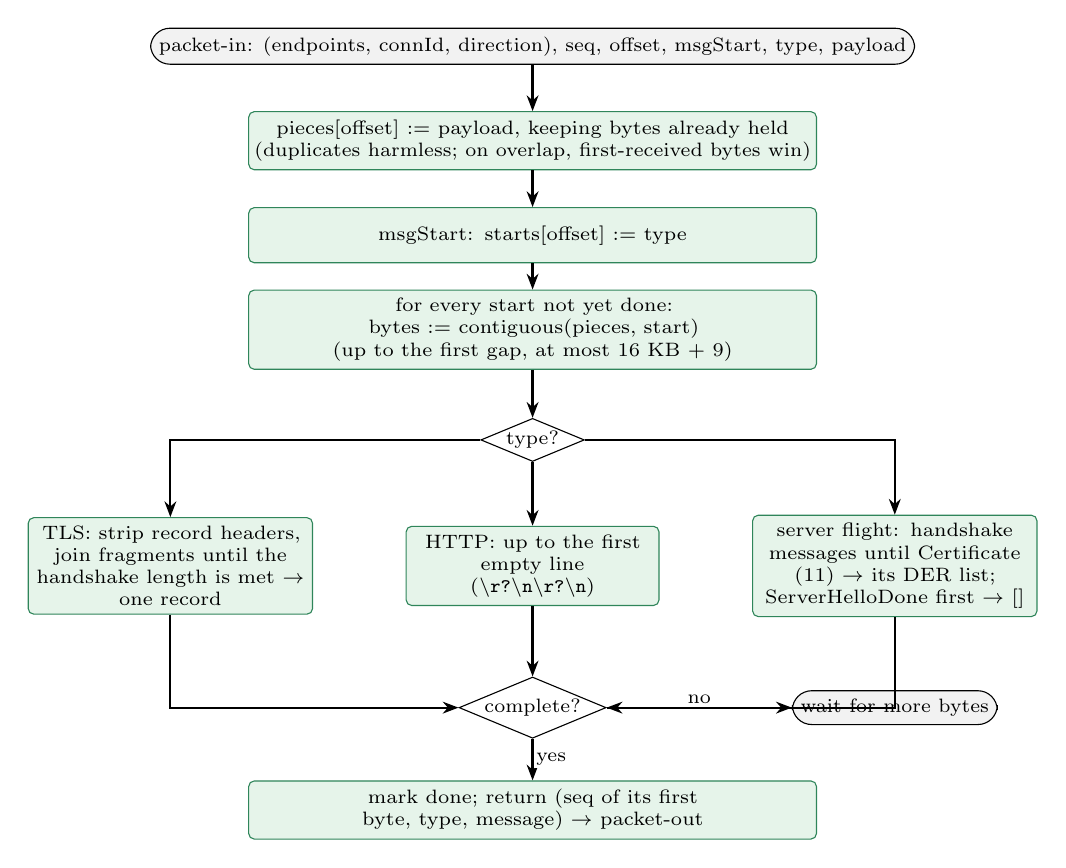
\begin{tikzpicture}
  \node[term] (in) at (0,0) {packet-in: (endpoints, connId, direction), seq, offset, msgStart, type, payload};
  \node[ctbox, text width=70mm] (keep) at (0,-1.2) {pieces[offset] := payload, keeping bytes already held\\ (duplicates harmless; on overlap, first-received bytes win)};
  \node[ctbox, text width=70mm] (st) at (0,-2.4) {msgStart: starts[offset] := type};
  \node[ctbox, text width=70mm] (loop) at (0,-3.6) {for every start not yet done: bytes := contiguous(pieces, start)\\ (up to the first gap, at most 16 KB + 9)};
  \node[dec] (k) at (0,-5.0) {type?};
  \node[ctbox, text width=34mm] (t) at (-4.6,-6.6) {TLS: strip record headers,\\ join fragments until the\\ handshake length is met $\to$\\ one record};
  \node[ctbox, text width=30mm] (h) at (0,-6.6) {HTTP: up to the first\\ empty line\\ (\code{\textbackslash r?\textbackslash n\textbackslash r?\textbackslash n})};
  \node[ctbox, text width=34mm] (f) at (4.6,-6.6) {server flight: handshake\\ messages until Certificate\\ (11) $\to$ its DER list;\\ ServerHelloDone first $\to$ []};
  \node[dec] (cpl) at (0,-8.4) {complete?};
  \node[term] (wait) at (4.6,-8.4) {wait for more bytes};
  \node[ctbox, text width=70mm] (out) at (0,-9.7) {mark done; return (seq of its first byte, type, message) $\to$ packet-out};
  \draw[arr] (in) -- (keep); \draw[arr] (keep) -- (st); \draw[arr] (st) -- (loop); \draw[arr] (loop) -- (k);
  \draw[arr] (k) -| (t); \draw[arr] (k) -- (h); \draw[arr] (k) -| (f);
  \draw[arr] (t) |- (cpl); \draw[arr] (h) -- (cpl); \draw[arr] (f) |- (cpl);
  \draw[arr] (cpl) -- node[lbl, above]{no} (wait); \draw[arr] (cpl) -- node[lbl, right]{yes} (out);
\end{tikzpicture}
\caption{\code{controller/reassembly.py}. It only knows framing (record headers, handshake lengths, the empty
line, DER lengths of the certificate list) and never interprets a fingerprint field. A ``start'' flagged on a short
segment that only looked like a message never completes and is ignored. Bounded: at most 32 KB per direction (lowest
offsets dropped first), a direction idle for 60\,s is dropped, at most 100,000 directions. The bytes of a joined
message are not dropped at once: a false start in the middle of a request can be ``joined'' before the real one,
whose first segment arrives last, and that one still needs them.}
\end{figure}

\subsection{TLS 1.2 certificates (JA4X) and the SSH flush}

\begin{figure}[H]\centering
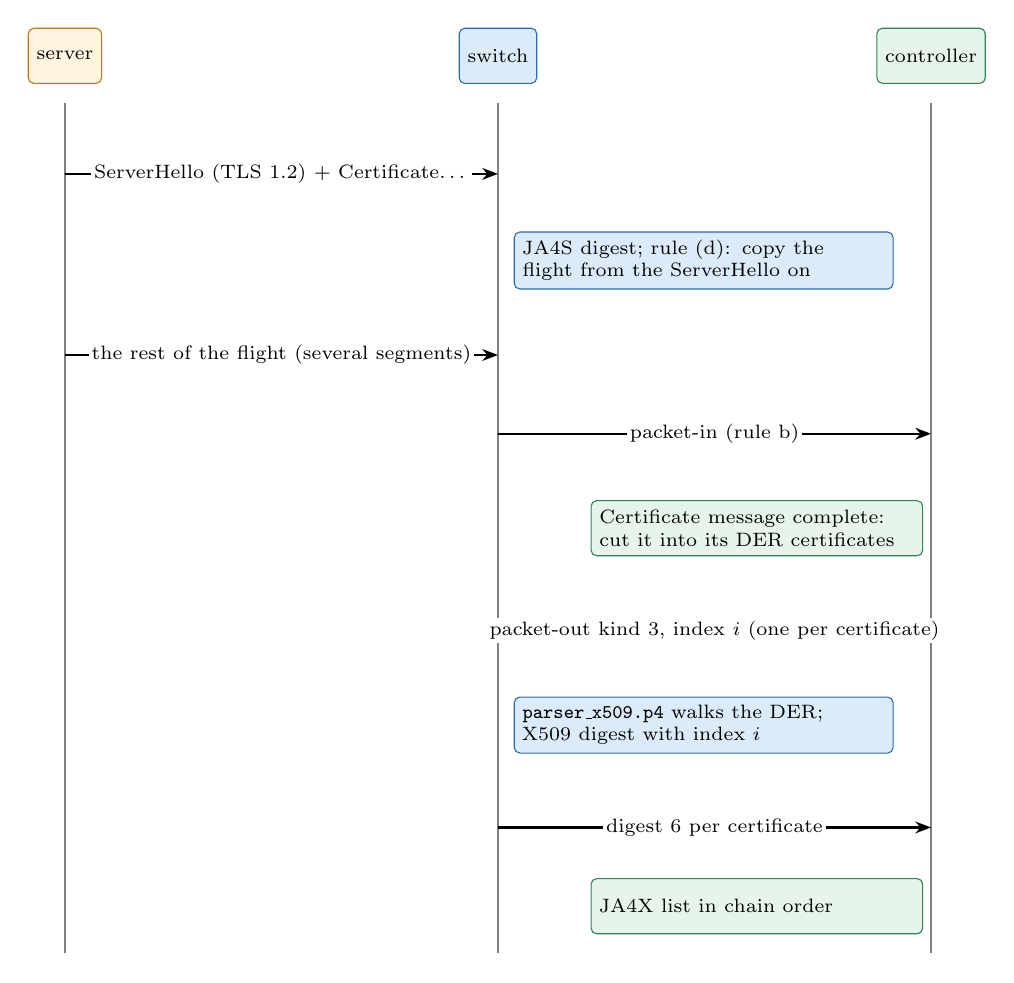
\begin{tikzpicture}[yscale=1.0]
  \node[hobox] (sv) at (0,0) {server};
  \node[swbox] (sw) at (5.5,0) {switch};
  \node[ctbox] (ct) at (11,0) {controller};
  \foreach \x in {0,5.5,11} \draw[thick, gray] (\x,-0.6) -- (\x,-11.4);
  \draw[arr] (0,-1.5) -- node[lbl]{ServerHello (TLS 1.2) + Certificate\ldots} (5.5,-1.5);
  \node[swbox, right, text width=46mm, align=left] at (5.7,-2.6) {JA4S digest; rule (d): copy the\\ flight from the ServerHello on};
  \draw[arr] (0,-3.8) -- node[lbl]{the rest of the flight (several segments)} (5.5,-3.8);
  \draw[arr] (5.5,-4.8) -- node[lbl]{packet-in (rule b)} (11,-4.8);
  \node[ctbox, left, text width=40mm, align=left] at (10.9,-6.0) {Certificate message complete:\\ cut it into its DER certificates};
  \draw[arr] (11,-7.3) -- node[lbl]{packet-out kind 3, index $i$ (one per certificate)} (5.5,-7.3);
  \node[swbox, right, text width=46mm, align=left] at (5.7,-8.5) {\code{parser\_x509.p4} walks the DER;\\ X509 digest with index $i$};
  \draw[arr] (5.5,-9.8) -- node[lbl]{digest 6 per certificate} (11,-9.8);
  \node[ctbox, left, text width=40mm, align=left] at (10.9,-10.8) {JA4X list in chain order};
\end{tikzpicture}
\caption{JA4X. Certificates are long (1--2 KB each) and always span segments, so they always take the join path.}
\end{figure}

\begin{figure}[H]\centering
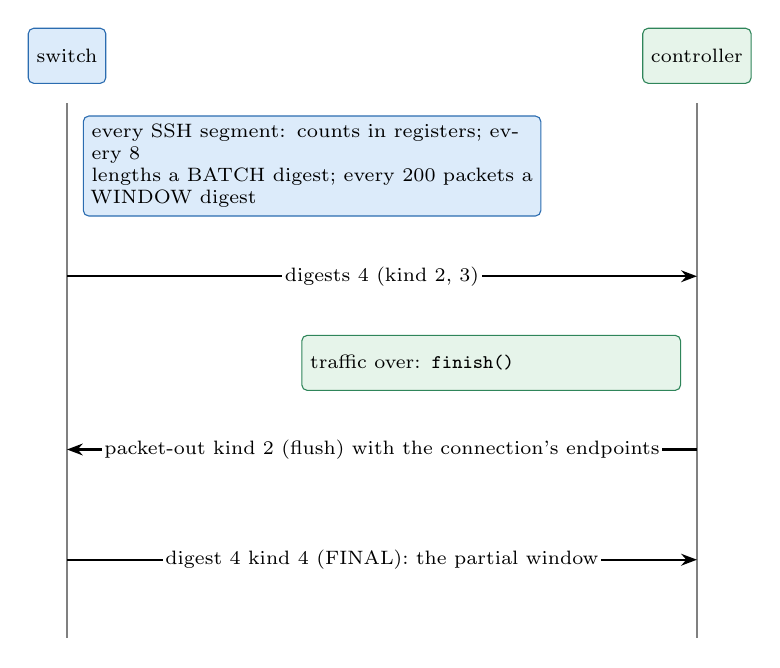
\begin{tikzpicture}[yscale=1.0]
  \node[swbox] (sw) at (0,0) {switch};
  \node[ctbox] (ct) at (8,0) {controller};
  \foreach \x in {0,8} \draw[thick, gray] (\x,-0.6) -- (\x,-7.4);
  \node[swbox, right, text width=56mm, align=left] at (0.2,-1.4) {every SSH segment: counts in registers; every 8\\ lengths a BATCH digest; every 200 packets a WINDOW digest};
  \draw[arr] (0,-2.8) -- node[lbl]{digests 4 (kind 2, 3)} (8,-2.8);
  \node[ctbox, left, text width=46mm, align=left] at (7.8,-3.9) {traffic over: \code{finish()}};
  \draw[arr] (8,-5.0) -- node[lbl]{packet-out kind 2 (flush) with the connection's endpoints} (0,-5.0);
  \draw[arr] (0,-6.4) -- node[lbl]{digest 4 kind 4 (FINAL): the partial window} (8,-6.4);
\end{tikzpicture}
\caption{The last JA4SSH window. FoxIO reports the partial last window at the end of its capture; P4Runtime on
BMv2 cannot read registers (UNIMPLEMENTED), so the switch is asked to report it itself.}
\end{figure}

%=====================================================================
\section{Each fingerprint, end to end}
\label{sec:fps}

Every fingerprint follows the same three steps: \textcolor{swd}{\textbf{the switch reads}} (parser + control,
state in registers), \textcolor{swd}{\textbf{sends a digest}}, \textcolor{ctd}{\textbf{the controller writes the
text}}. The figures show each step and the anatomy of the result.

\newcommand{\fpstrip}[4]{%
\begin{tikzpicture}
  \node[swbox, text width=46mm, align=left, minimum height=20mm] (a) at (0,0) {#1};
  \node[swbox, text width=40mm, align=left, minimum height=20mm] (b) at (5.4,0) {#2};
  \node[ctbox, text width=46mm, align=left, minimum height=20mm] (c) at (10.8,0) {#3};
  \draw[arr] (a) -- (b); \draw[arr] (b) -- node[lbl, above=2mm]{digest} (c);
  \node[fibox, text width=158mm, align=left, font=\scriptsize] at (5.4,-1.75) {#4};
\end{tikzpicture}}

\subsection{JA4T, JA4TS, JA4L: the TCP handshake}

\begin{figure}[H]\centering
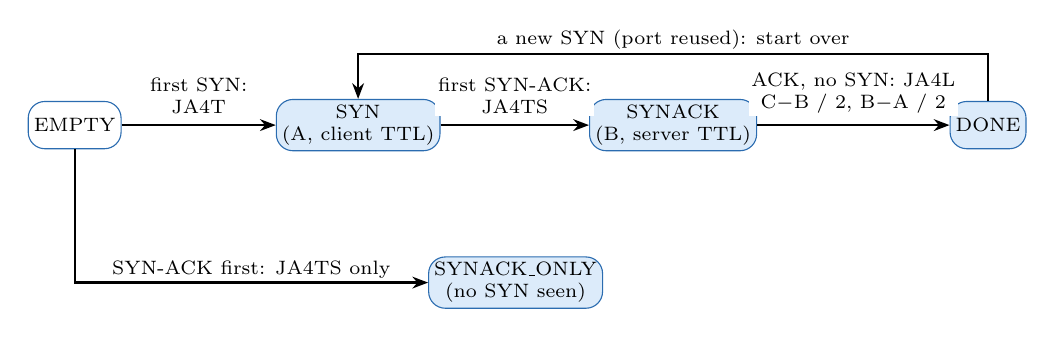
\begin{tikzpicture}
  \node[st, fill=white] (e) at (0,0) {EMPTY};
  \node[st] (syn) at (3.6,0) {SYN\\ (A, client TTL)};
  \node[st] (sa) at (7.6,0) {SYNACK\\ (B, server TTL)};
  \node[st] (done) at (11.6,0) {DONE};
  \node[st] (so) at (5.6,-2.0) {SYNACK\_ONLY\\ (no SYN seen)};
  \draw[arr] (e) -- node[lbl, above=1mm]{first SYN:\\ JA4T} (syn);
  \draw[arr] (syn) -- node[lbl, above=1mm]{first SYN-ACK:\\ JA4TS} (sa);
  \draw[arr] (sa) -- node[lbl, above=1mm]{ACK, no SYN: JA4L\\ C$-$B / 2, B$-$A / 2} (done);
  \draw[arr] (e) |- node[lbl, pos=0.75, above]{SYN-ACK first: JA4TS only} (so);
  \draw[arr] (done.north) -- ++(0,0.6) -| node[lbl, pos=0.25, above]{a new SYN (port reused): start over} (syn.north);
\end{tikzpicture}
\caption{\code{p4/handshake.p4}: one state per connection slot. A repeated SYN or SYN-ACK changes nothing (the
reference also takes the first). Time = the switch's ingress timestamp in microseconds.}
\end{figure}

\begin{figure}[H]\centering
\fpstrip{\textbf{parser}: every TCP option byte; kinds in order, MSS (kind 2), window scale (kind 3); window from
the TCP header}{\textbf{Handshake}: state machine above; timestamps and TTLs in registers; JA4L computed in the
switch}{\textbf{handshake.py}: \code{window\_kinds\_mss\_scale}; JA4L: \code{latency\_ttl} for each half}%
{JA4T = \textbf{64240}\_\textbf{2-4-8-1-3}\_\textbf{1460}\_\textbf{7}: window \_ option kinds in order \_ MSS \_ window
scale (00 if absent) \quad JA4TS: same, of the SYN-ACK \quad JA4L-C = \textbf{1320}\_\textbf{64}: (ACK $-$ SYN-ACK)/2
in $\mu$s \_ client TTL; JA4L-S: (SYN-ACK $-$ SYN)/2 \_ server TTL}
\end{figure}

\subsection{JA4 and JA4S: TLS hellos}
\begin{figure}[H]\centering
\fpstrip{\textbf{parser\_tls.p4}: complete hello only; legacy and supported versions, SNI present, every cipher
and extension (GREASE out), signature algorithms, first ALPN name}{\textbf{Tls}: once per connection and
direction (\code{tlsDone} bits); a split hello is walked when the controller sends it back}{\textbf{tls.py}: version
code, counts, ALPN chars; sorted ciphers and extensions (SNI, ALPN out); SHA-256, 12 hex digits}%
{JA4 = \textbf{t13d1516h2}\_\textbf{8daaf6152771}\_\textbf{02713d6af862}: t = TCP, 13 = TLS 1.3, d = SNI present
(i: absent), 15 ciphers, 16 extensions, h2 = first and last character of the first ALPN \_ hash(sorted ciphers) \_
hash(sorted extensions \_ signature algorithms in order)\quad JA4S = \textbf{t130200}\_\textbf{1302}\_\textbf{a56c5b993250}:
version, extension count, ALPN \_ chosen cipher \_ hash(extensions in order)}
\end{figure}

\subsection{JA4H: HTTP requests}
\begin{figure}[H]\centering
\fpstrip{\textbf{parser\_http.p4}: method, version, every header name (case kept), Cookie pairs, Accept-Language
(4 chars), Referer present}{\textbf{Http}: one per request; a retransmission (same sequence number) not twice;
serial number; the request's sequence number}{\textbf{http.py}: method code, version, flags, count, language;
hash(names), hash(sorted cookie names), hash(sorted cookie pairs); a connection's list kept in stream order}%
{JA4H = \textbf{ge11cr04engb}\_\textbf{8ddaef5d77af}\_\textbf{3645093e176f}\_\textbf{b1c22010166d}: ge = GET, 11 =
HTTP/1.1, c = cookie, r = referer, 04 headers (without Cookie, Referer), engb = language \_ hash(header names in
order) \_ hash(sorted cookie names) \_ hash(sorted cookie name=value pairs)}
\end{figure}

\subsection{JA4SSH: SSH packet sizes}
\begin{figure}[H]\centering
\fpstrip{\textbf{parser}: TCP on port 22, or a connection whose data begins with ``SSH-'' (any port; bare ACKs
before the banner count too). An SSH packet = a segment with payload; a bare ACK = no payload, flags exactly ACK}{\textbf{Ssh}: counts per direction; lengths in batches of 8; window closes at 200 SSH packets;
flush at the end}{\textbf{ssh.py}: histogram of the window's lengths per direction; mode (smallest on a tie)}%
{JA4SSH = \textbf{c36s52}\_\textbf{c100s100}\_\textbf{c0s0}: most frequent client / server payload length \_ client /
server SSH packets \_ client / server bare ACKs (one value per window of 200 packets)}
\end{figure}

\subsection{JA4D and JA4D6: DHCP}
\begin{figure}[H]\centering
\fpstrip{\textbf{parser\_dhcp.p4}: v4 options after the 240-byte header; v6 options including nested ones in
packet order}{\textbf{Dhcp}: one digest per message (not a connection); serial number}{\textbf{dhcp.py}: type name
(5 letters), size, flags, lists joined by '-'}%
{JA4D = \textbf{disco0576nn}\_\textbf{57-55-60-61}\_\textbf{1-3-6-12-15-28-42}: type, max message size (v6: DUID
length), i = requested IP (v6: IA\_TA), d = a domain name in the FQDN option \_ option codes (v4 without 0, 50, 53, 81,
255) \_ requested codes}
\end{figure}

\subsection{JA4X: certificates}
\begin{figure}[H]\centering
\fpstrip{\textbf{parser\_x509.p4}: the DER walk of one certificate sent back by the controller; OIDs of issuer,
subject, extensions}{\textbf{X509}: one digest per certificate, with its index in the chain}{\textbf{x509.py}: each
OID as hex, joined by ','; SHA-256, 12 hex digits per list}%
{JA4X = \textbf{a373a9f83c6b}\_\textbf{2e9214a636bc}\_\textbf{a4df8b54db06}: hash(issuer attribute OIDs) \_
hash(subject attribute OIDs) \_ hash(extension OIDs), per certificate of a TLS 1.2 (or older) chain}
\end{figure}

%=====================================================================
\section{How correctness is checked}
\label{sec:verif}\label{sec:testing}

\subsection{The replay bench (no root)}
\begin{figure}[H]\centering
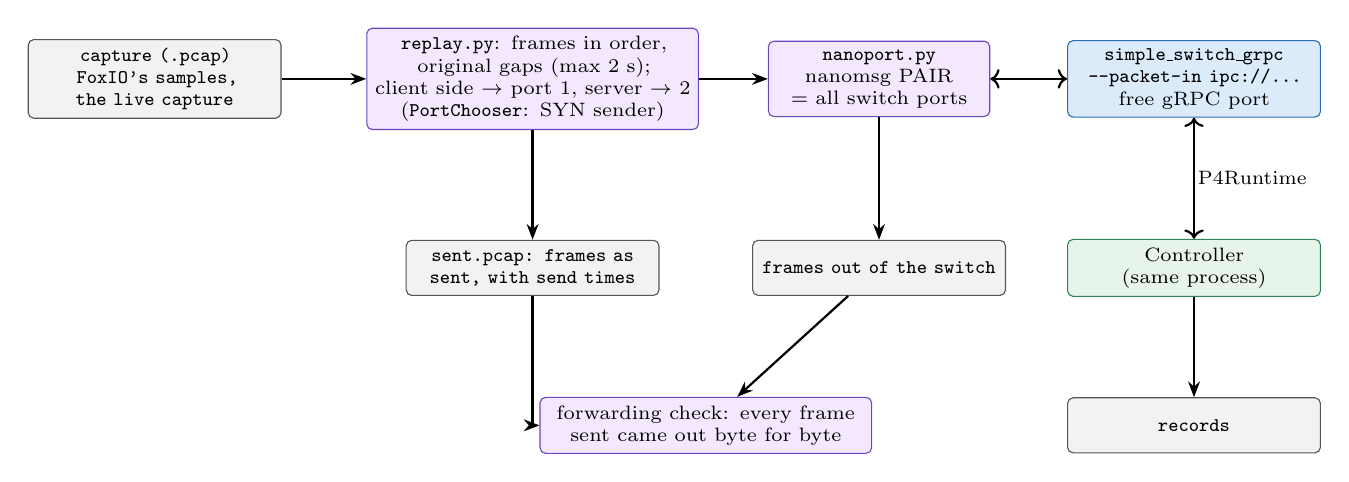
\begin{tikzpicture}
  \node[fibox, text width=30mm] (pcap) at (0,0) {capture (.pcap)\\ FoxIO's samples,\\ the live capture};
  \node[rfbox, text width=40mm] (rp) at (4.8,0) {\code{replay.py}: frames in order,\\ original gaps (max 2 s);\\ client side $\to$ port 1, server $\to$ 2\\ (\code{PortChooser}: SYN sender)};
  \node[rfbox, text width=26mm] (nn) at (9.2,0) {\code{nanoport.py}\\ nanomsg PAIR\\ = all switch ports};
  \node[swbox, text width=30mm] (sw) at (13.2,0) {\code{simple\_switch\_grpc}\\ \code{--packet-in ipc://\ldots}\\ free gRPC port};
  \node[ctbox, text width=30mm] (ct) at (13.2,-2.4) {Controller\\ (same process)};
  \node[fibox, text width=30mm] (sent) at (4.8,-2.4) {sent.pcap: frames as\\ sent, with send times};
  \node[fibox, text width=30mm] (out) at (9.2,-2.4) {frames out of the switch};
  \node[fibox, text width=30mm] (recs) at (13.2,-4.4) {records};
  \node[rfbox, text width=40mm] (fw) at (7.0,-4.4) {forwarding check: every frame\\ sent came out byte for byte};
  \draw[arr] (pcap) -- (rp); \draw[arr] (rp) -- (nn); \draw[arr, <->] (nn) -- (sw);
  \draw[arr, <->] (sw) -- node[lbl, right]{P4Runtime} (ct); \draw[arr] (ct) -- (recs);
  \draw[arr] (rp) -- (sent); \draw[arr] (nn) -- (out);
  \draw[arr] (sent) |- (fw); \draw[arr] (out) -- (fw);
\end{tikzpicture}
\caption{\code{tools/replay.py}. The real switch binary and the real controller, without network namespaces: BMv2's
\code{--packet-in} option makes one nanomsg socket stand for all its ports. A warm-up frame goes first (the first
frame after loading the program reaches the pipeline late). The switch dies with its parent
(\code{PR\_SET\_PDEATHSIG}), so no run can leave one behind.}
\end{figure}

\subsection{Comparison against independent references}
\begin{figure}[H]\centering
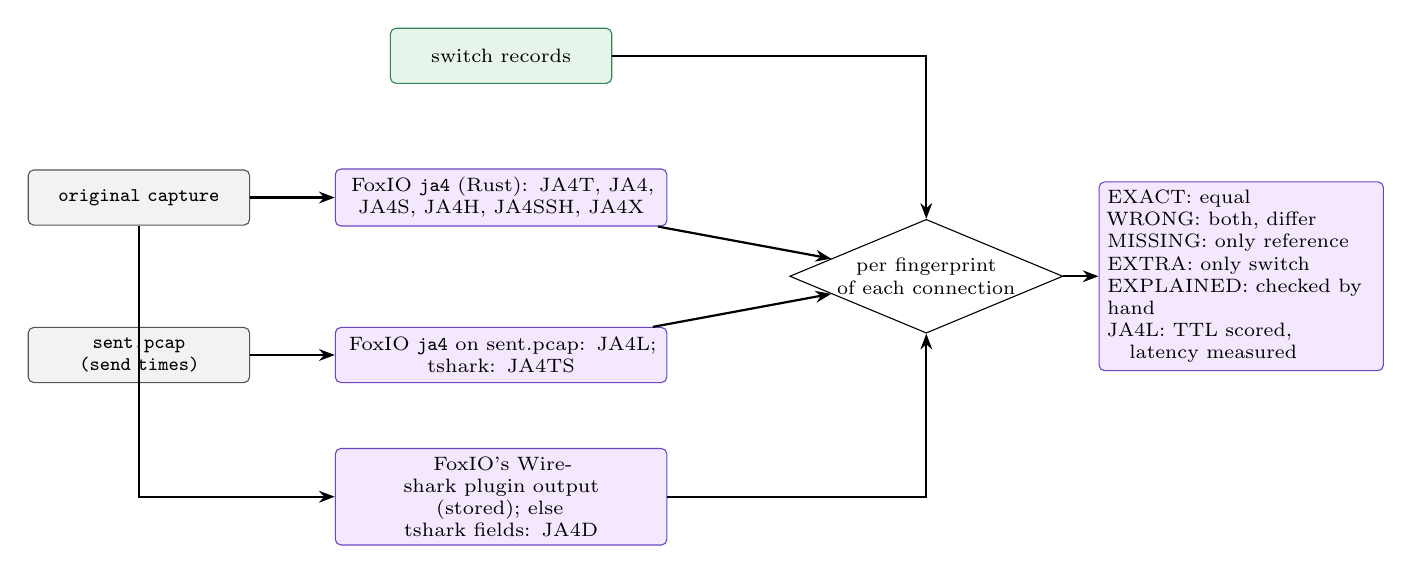
\begin{tikzpicture}
  \node[fibox, text width=26mm] (o) at (0,0) {original capture};
  \node[fibox, text width=26mm] (s) at (0,-2.0) {sent.pcap\\ (send times)};
  \node[rfbox, text width=40mm] (fx) at (4.6,0) {FoxIO \code{ja4} (Rust): JA4T, JA4,\\ JA4S, JA4H, JA4SSH, JA4X};
  \node[rfbox, text width=40mm] (fl) at (4.6,-2.0) {FoxIO \code{ja4} on sent.pcap: JA4L;\\ tshark: JA4TS};
  \node[rfbox, text width=40mm] (fd) at (4.6,-3.8) {FoxIO's Wireshark plugin output\\ (stored); else tshark fields: JA4D};
  \node[ctbox, text width=26mm] (sw) at (4.6,1.8) {switch records};
  \node[dec] (v) at (10.0,-1.0) {per fingerprint\\ of each connection};
  \node[rfbox, text width=34mm, align=left] (verd) at (14.0,-1.0) {EXACT: equal\\ WRONG: both, differ\\ MISSING: only reference\\ EXTRA: only switch\\ EXPLAINED: checked by hand\\ JA4L: TTL scored,\\ \quad latency measured};
  \draw[arr] (o) -- (fx); \draw[arr] (s) -- (fl); \draw[arr] (o) |- (fd);
  \draw[arr] (fx) -- (v); \draw[arr] (fl) -- (v); \draw[arr] (fd) -| (v); \draw[arr] (sw) -| (v);
  \draw[arr] (v) -- (verd);
\end{tikzpicture}
\caption{\code{tools/compare.py} with \code{tools/reference.py}. JA4 values come from the original capture
(timing-free); JA4L and JA4TS from the frames as the switch received them, so both sides time the same packets.}
\end{figure}

\subsection{The live run (root)}
\begin{figure}[H]\centering
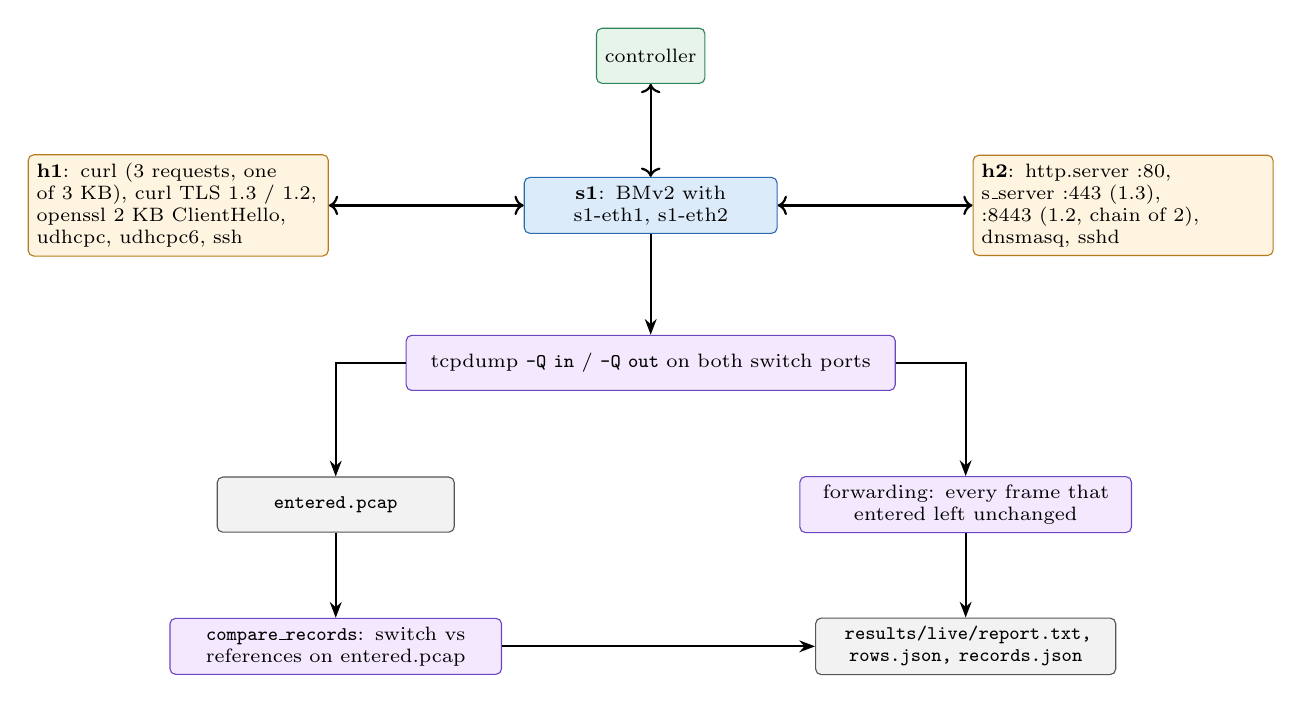
\begin{tikzpicture}
  \node[hobox, text width=36mm, align=left] (h1) at (0,0) {\textbf{h1}: curl (3 requests, one\\ of 3 KB), curl TLS 1.3 / 1.2,\\ openssl 2 KB ClientHello,\\ udhcpc, udhcpc6, ssh};
  \node[swbox, text width=30mm] (s1) at (6,0) {\textbf{s1}: BMv2 with\\ s1-eth1, s1-eth2};
  \node[hobox, text width=36mm, align=left] (h2) at (12,0) {\textbf{h2}: http.server :80,\\ s\_server :443 (1.3),\\ :8443 (1.2, chain of 2),\\ dnsmasq, sshd};
  \node[ctbox] (ct) at (6,1.9) {controller};
  \node[rfbox, text width=60mm] (td) at (6,-2.0) {tcpdump \code{-Q in} / \code{-Q out} on both switch ports};
  \node[fibox, text width=28mm] (en) at (2,-3.8) {entered.pcap};
  \node[rfbox, text width=40mm] (fwd) at (10,-3.8) {forwarding: every frame that\\ entered left unchanged};
  \node[rfbox, text width=40mm] (cmp) at (2,-5.6) {\code{compare\_records}: switch vs\\ references on entered.pcap};
  \node[fibox, text width=36mm] (rep) at (10,-5.6) {results/live/report.txt,\\ rows.json, records.json};
  \draw[arr, <->] (h1) -- (s1); \draw[arr, <->] (s1) -- (h2); \draw[arr, <->] (s1) -- (ct);
  \draw[arr] (s1) -- (td); \draw[arr] (td) -| (en); \draw[arr] (td) -| (fwd);
  \draw[arr] (en) -- (cmp); \draw[arr] (cmp) -- (rep); \draw[arr] (fwd) -- (rep);
\end{tikzpicture}
\caption{\code{network/run\_live.py}: real programs, real TCP stacks (offloads off, so TCP itself splits the large
messages), the same switch and controller. The clients start only when h2 listens on every server port; every
client runs under \code{timeout} and its exit status is checked (a failed step is reported); every server's process
id is kept and only those processes are stopped. \code{tools/live\_tex.py} then writes the results table from \code{rows.json}.}
\end{figure}

\subsection{The tests: what each one protects}
\begin{center}\footnotesize
\begin{tabularx}{\textwidth}{l >{\raggedright\arraybackslash}X >{\raggedright\arraybackslash}p{38mm}}
\toprule
\textbf{test} & \textbf{what it sends and expects} & \textbf{protects} \\
\midrule
\code{test\_split\_reorder} & real hellos and requests cut into 2--5 pieces: in order, reversed, every permutation of 3, duplicated, overlapping, after 20 other bytes, without the SYN; expected = FoxIO on the message sent whole. 202 cases exact; 8 known limit cases must never be wrong & Stream, Reassembler, the parsers on joined messages \\
\code{test\_server\_flight\_reorder} & h2's TLS 1.2 flight from the live run (ServerHello, chain of 2, 2,241 bytes) cut as TCP cut it, in every order of 3 pieces, in 100-byte pieces reversed, duplicated, overlapping; expected = FoxIO on the flight sent whole. 19 cases exact; a split ServerHello: JA4S exact, JA4X never wrong & rules (c), (d), (b) for the server; the flight's join \\
\code{test\_keepalive\_reorder} & on one connection: a whole request, a second request cut into 2 or 3 pieces in 18 orders, a third whole; expected = FoxIO's three JA4H on the requests sent whole, in order. 18 cases exact & rule (e); JA4H in stream order \\
\code{test\_port\_reuse} & two TLS connections and two SSH sessions, each pair on one four-tuple (FIN, then a new SYN; one SYN repeated); compared with FoxIO by stream & ConnId; records per connection; SSH window on reuse \\
\code{test\_vlan\_and\_ssh\_port} & TLS in one 802.1Q tag, HTTP in 802.1ad + 802.1Q, the live SSH session on port 2222; compared with FoxIO & VLAN parsing; SSH by banner \\
\code{test\_controller\_state} & reassembler alone, with a clock passed in: 300 split requests on one connection, an idle direction, 1,000 directions, 100 KB without a start, a false start inside a request & D24 bounds; no early pruning \\
\code{test\_ja4l\_gaps} & a handshake with 1\,s and 0.5\,s gaps; JA4L within 2\%; JA4T/JA4TS exact & Handshake arithmetic (halving, order) \\
\code{test\_one\_digest\_per\_packet} & a whole ClientHello / HTTP request on the handshake's ACK: JA4L and the message's fingerprint both reported & the deferred handshake digest \\
\code{test\_identical\_digests} & 3 identical DHCP offers, 3 identical HTTP requests, 4 identical SSH windows (acknowledgements held back) & the serial numbers \\
\code{test\_dhcp6\_fqdn} & option 39 with an empty and a real name: \code{n}, \code{d} & the JA4D6 domain flag \\
\code{test\_capacity\_limits} & lists at and one past each capacity: exact, then ``incomplete'' & every overflow path \\
\bottomrule
\end{tabularx}
\end{center}

\subsection{The measurement study}
\begin{figure}[H]\centering
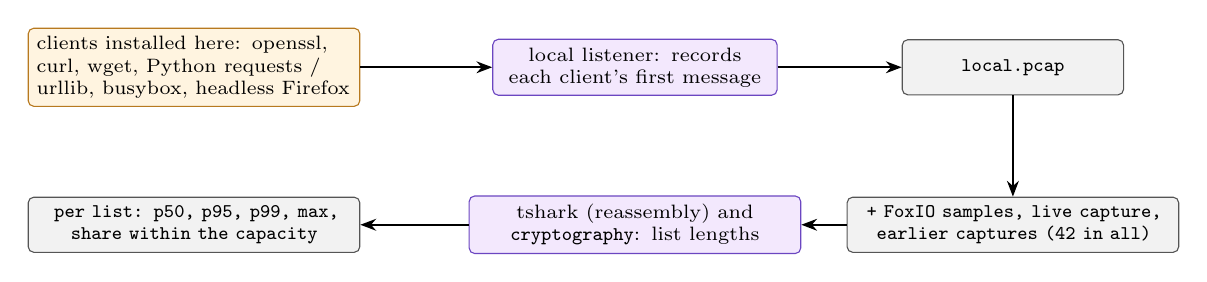
\begin{tikzpicture}
  \node[hobox, text width=40mm, align=left] (cl) at (0,0) {clients installed here: openssl,\\ curl, wget, Python requests /\\ urllib, busybox, headless Firefox};
  \node[rfbox, text width=34mm] (rec) at (5.6,0) {local listener: records\\ each client's first message};
  \node[fibox, text width=26mm] (lp) at (10.4,0) {local.pcap};
  \node[fibox, text width=40mm] (cor) at (10.4,-2.0) {+ FoxIO samples, live capture,\\ earlier captures (42 in all)};
  \node[rfbox, text width=40mm] (cnt) at (5.6,-2.0) {tshark (reassembly) and\\ \code{cryptography}: list lengths};
  \node[fibox, text width=40mm] (res) at (0,-2.0) {per list: p50, p95, p99, max,\\ share within the capacity};
  \draw[arr] (cl) -- (rec); \draw[arr] (rec) -- (lp); \draw[arr] (lp) -- (cor); \draw[arr] (cor) -- (cnt); \draw[arr] (cnt) -- (res);
\end{tikzpicture}
\caption{\code{tools/measure\_field\_counts.py}: are the switch's capacities large enough? (Results:
Section~\ref{sec:results}.)}
\end{figure}


\part{Explanation}
%=====================================================================
\section{The problem and the scope}
\label{sec:problem}

\textbf{Goal (as set by the faculty).} A linear network with one switch and two hosts (h1 -- s1 -- h2). Traffic
flows between the hosts; the switch computes every JA4+ fingerprint it can, with P4, \emph{correctly}, including
when a message is split over several packets or its packets arrive out of order (``the server's 2nd packet may
come first''). A controller is part of the design, so that higher-level programs can drive the switch. Nothing
else: no attack mitigation, no flood protection, no hardware port. The contribution: JA4+ fingerprinting done in
the P4 data plane.

\textbf{What is fingerprinted.} Before a protocol's session is encrypted (or for protocols that are never
encrypted), the two sides exchange clear-text messages whose structure depends on the software that sent them:

\begin{center}\footnotesize
\begin{tabularx}{\textwidth}{l >{\raggedright\arraybackslash}X l l}
\toprule
\textbf{Fingerprint} & \textbf{clear-text exchange read} & \textbf{per} & \textbf{reference} \\
\midrule
JA4T / JA4TS & client SYN / server SYN-ACK: window, TCP options, MSS, window scale & connection & FoxIO \code{ja4}; tshark \\
JA4L-C / -S & timing of SYN, SYN-ACK, ACK and the TTLs & connection & FoxIO \code{ja4} \\
JA4 / JA4S & TLS ClientHello / ServerHello (all versions; the hellos are always clear) & connection & FoxIO \code{ja4} \\
JA4H & HTTP/1.x request header block & request & FoxIO \code{ja4} \\
JA4SSH & sizes and directions of SSH packets (SSH payload is encrypted after key exchange) & 200 packets & FoxIO \code{ja4} \\
JA4D / JA4D6 & DHCP / DHCPv6 messages (never encrypted) & message & FoxIO's Wireshark plugin \\
JA4X & certificates in a TLS 1.2 (or older) server flight & certificate & FoxIO \code{ja4} \\
\bottomrule
\end{tabularx}
\end{center}

\textbf{Out of reach, by nature:} HTTP/2 and HTTP/3 requests and TLS 1.3 certificates are inside encryption (FoxIO's
tool computes them only for captures that store the session keys). \textbf{Not implemented, by scope:} JA4 over QUIC
(its ClientHello is in Initial packets whose keys are derived from public values: readable passively, but v1model
has no AES or HKDF, so it would need the controller to decrypt), JA4 over DTLS, tunnels (GRE, VXLAN, Geneve: the
inner headers would need a second parser path), IPv6 extension headers. Section~\ref{sec:coverage} lists what is
done and what is not, with the reason and what doing it would take.

\textbf{Target.} BMv2 (\code{simple\_switch\_grpc}), the P4-16 v1model architecture, P4Runtime over gRPC. BMv2 is
the reference software switch of P4; a hardware target (Tofino) has different limits and is not part of this
project.

\textbf{What ``correct'' means here.} For every fingerprint, the switch's value equals the value FoxIO's own tools
compute on the same frames, character for character; and every frame leaves the switch unchanged. JA4L is a time
measurement, so its TTL part must be equal and its latency is reported as a difference distribution (BMv2 timestamps
a packet when its pipeline takes it up, which a software switch delays by microseconds to milliseconds).

%=====================================================================
\section{Design decisions: what, why, and why not the alternatives}
\label{sec:decisions}

Each decision is stated, then the reason, then the alternatives that were considered and why they were not taken.

\newcommand{\decision}[4]{%
\subsection{#1}#2
\par\noindent\textbf{Decision.} #3
\par\noindent\textbf{Why.} #4}

\decision{D1. BMv2, v1model and a P4Runtime controller}{\label{sec:dec-target}}
{The switch is BMv2's \code{simple\_switch\_grpc} running a P4-16 v1model program; a Python controller talks to it
over P4Runtime.}
{BMv2 is the reference P4 target, runs anywhere, needs no hardware, and supports everything the design uses:
parser loops with \code{lookahead}/\code{advance}, registers, hashes, digests, resubmit, clone, packet-in/out.
P4Runtime is the standard control interface, so ``a high-level program drives the switch'' means exactly: another
P4Runtime client, or this controller's Python API.}
\whynot{\emph{Tofino}: hardware limits (parser depth, stages, no 2,048-bit fields) would dominate the work; the
faculty asked for fingerprinting, not a hardware port. \emph{eBPF/XDP}: not P4. \emph{Other P4 architectures}: v1model is the one
\code{simple\_switch\_grpc} implements completely (resubmit, clone with preserved metadata, digests); PSA support in
BMv2 is a separate, less complete switch, and TNA is Tofino's.}

\decision{D2. The parser reads every fingerprint value}{\label{sec:dec-parser}}
{All variable-length reading (TCP options, TLS lists, HTTP headers, DHCP options, DER) is done by P4 parser states.
The controller never parses a fingerprint field.}
{This is the contribution: fingerprinting in the data plane. The parser is the only P4 block that can loop over a
variable number of items (a state may transition to itself).}
\whynot{\emph{Send every packet to the controller and parse there}: a software fingerprinter with a switch in front.
\emph{Parse with match-action tables}: tables match fixed offsets; variable-length lists need the parser's loops.}

\decision{D3. Results leave the switch as digests}{\label{sec:dec-digest}}
{Each control sends its values in one digest struct (six kinds), as soon as they are complete.}
{A digest carries only the extracted values (a few hundred bytes), asynchronously, without the packet; the packet
is forwarded at once. It is P4Runtime's standard channel for data-plane-to-controller events.}
\whynot{\emph{Packet-in of every interesting packet}: sends the whole packet and makes the controller parse.
\emph{Controller reads registers}: BMv2's P4Runtime server answers UNIMPLEMENTED for register reads (found, see
the problems table), and polling would race with new connections. \emph{Write results into a header and mirror}:
needs a custom receiver and still a clone per message.}

\decision{D4. Sorting, SHA-256 and text in the controller}{\label{sec:dec-hash}}
{The switch sends lists in packet order; the controller sorts the cipher and extension lists, hashes with SHA-256 and
writes FoxIO's text.}
{v1model has no SHA-256 extern, no strings, and no loops in the pipeline (only in the parser). The fingerprint is
fully determined by the values the switch extracted; sorting and hashing them anywhere gives the same result.}
\whynot{\emph{A sorting network in P4} (bitonic, as in the earlier ja4p4 plan): needed on a Tofino to report sorted
lists from the data plane; on BMv2 it adds hundreds of compare-and-swap actions and proves nothing about
fingerprinting. \emph{A CRC instead of SHA-256}: would not be JA4 and could not be compared with FoxIO.}

\decision{D5. Walked packets are resubmitted and forwarded on a second pass}{\label{sec:dec-resubmit}}
{A parser walk skips bytes with \code{advance}; the packet is then resubmitted, and on the second pass only
Ethernet is parsed, so the original bytes are forwarded.}
{\code{advance} removes the skipped bytes from what the deparser emits. Resubmit runs the original packet through
the pipeline again, with chosen metadata preserved (field list 0: arrival port, the pending handshake record).}
\whynot{\emph{Extract every byte into headers}: thousands of header-stack entries; the deparser would re-emit them
(the TCP option walk does extract, since options are at most 40 bytes). \emph{Recirculate}: passes through egress
and the deparser, which would emit the shortened packet.}

\decision{D6. Split and out-of-order messages are joined by the controller and read by the switch}{\label{sec:dec-join}}
{The switch decides which segments may hold pieces of a message (Fig.~\ref{fig:copyrules}) and copies them with
their stream offset; the controller orders the bytes by framing only and sends the complete message back; the
same parser reads it.}
{A P4 switch processes one packet at a time and cannot hold a packet back or keep kilobytes of payload per
connection. Joining needs a buffer; reading does not. So the buffer is in the controller and the reading stays in
P4. The controller's join is framing only (record headers, the empty line, DER lengths), never a fingerprint field.}
\whynot{\emph{Buffer segments in registers}: a ClientHello reaches 2 KB, certificates many KB; registers sized for
that per connection are impossible on hardware and costly on BMv2, and register access is per packet, fixed-width.
\emph{Parse each piece separately and merge partial states}: a list value can be cut in the middle and the order of
pieces is unknown; the state machine would need to be resumable at every byte in both orders. \emph{Ignore split
messages}: wrong by omission for exactly the cases the faculty named.}

\decision{D7. Copies are made at egress (E2E clone)}{\label{sec:dec-e2e}}
{\code{clone\_preserving\_field\_list(CloneType.E2E, 100, 1)} in egress; the clone gets the \code{packet\_in}
header.}
{An ingress-to-egress clone is parsed again from the start, and its walk consumes the bytes again: the copy
arrived without payload (found by the tests). At egress the packet has all its bytes.}

\decision{D8. Per-connection state in hashed register slots}{\label{sec:dec-slots}}
{ConnKey orders the endpoints, hashes them (CRC16 slot, CRC32 check); every control keeps its state in register
arrays of 65,536 entries indexed by the slot, together with the connection's number (D21).}
{A P4 program cannot add table entries; registers are the data plane's writable memory. Ordering the endpoints
makes both directions find the same slot. The 32-bit check tells two connections in one slot apart.}
\whynot{\emph{One table entry per connection from the controller}: a round trip before the first packet's state
exists, and the SYN's timestamp would be lost. \emph{Bigger slots / buckets}: unneeded for one link; one constant.}

\decision{D9. One \code{digest()} call per control; the handshake digest sent last}{\label{sec:dec-onedigest}}
{Every control has exactly one digest call; the handshake record is stored in metadata and sent from a single call
at the end of ingress, on the second pass if this pass sent a message digest.}
{p4c makes one learn list per call site (a second call site of the same struct is a different list the controller
did not enable), and BMv2 keeps \emph{one digest per packet}: the handshake's ACK can carry a whole ClientHello, and
its JA4L would be lost (found with SSH, then covered by \code{test\_one\_digest\_per\_packet}).}

\decision{D10. A serial number in DHCP, HTTP and SSH digests}{\label{sec:dec-serial}\label{sec:serial}}
{A 32-bit counter register per digest kind; each digest carries its value.}
{BMv2 keeps every digest until it is acknowledged and drops a new one identical to it. Identical messages close
together (DHCP retransmissions and their answers, the same HTTP request repeated, identical SSH windows of a bulk
transfer) were lost. 32 bits: the serial need only differ among digests unacknowledged at the same time (rate
$\times$ acknowledgement time, below $2^{20}$ even at $10^6$/s for 1\,s); wrapping at $2^{32}$ is harmless and needs
no flag, because the controller never reads the value.}
\whynot{\emph{Acknowledge faster}: the filter exists until the acknowledgement arrives, however fast. \emph{Use the
timestamp}: two packets in one microsecond collide. \emph{Per-connection counters}: DHCP has no connection.}

\decision{D11. GREASE is recognised in the parser's \code{select}}{}
{\code{IS\_GREASE(v)}: low nibbles of both bytes are 0xA and the two bytes are equal; the value is skipped before
it is stored.}
{GREASE is a bit pattern, not a lookup; a \code{select} on it costs nothing and keeps the lists clean, so counts
are right without a second pass.}
\whynot{\emph{A match-action table marking slots invalid}: needs a list of slots to filter afterwards and then
compaction; the parser simply never stores them.}

\decision{D12. Capacities: 128 / 64 / 64 values, 512 / 1,024 / 256 bytes, then ``incomplete''}{}
{Each list is kept in fixed-width fields (at most 2,048 bits each, chained); past its capacity the count stays
right, an overflow bit is set, and the fingerprint is reported as incomplete.}
{A wrong fingerprint is worse than none. The capacities were checked by a measurement study (every one of 1,238
measured lists fits; closest: cookies 863 of 1,024 bytes, ciphers 86 of 128) and the overflow path by
\code{test\_capacity\_limits}.}
\whynot{\emph{Larger capacities}: cost digest bits and parser iterations for no measured case. \emph{Truncate
silently}: would give wrong hashes.}

\decision{D13. JA4L timed in the switch}{}
{The switch stores the SYN and SYN-ACK times and TTLs and computes both halves when the ACK passes.}
{The point of JA4L is the network position of the measuring device; the switch is that device. The controller
would see digests later and with its own jitter.}
\whynot{\emph{Controller time}: measures the control channel, not the network. Limit kept honest: BMv2 stamps when
its pipeline takes the packet up, so the latency is reported as a measurement and the arithmetic is tested with
known gaps.}

\decision{D14. SSH: counts in the switch, the mode in the controller}{}
{The switch counts SSH packets and bare ACKs per direction and window exactly, and sends the payload lengths in
batches of 8; the controller computes the most frequent length.}
{A mode needs a histogram over arbitrary lengths; a data plane has no dynamic map. Everything else of JA4SSH is
counting, which registers do exactly.}
\whynot{\emph{A fixed histogram in registers}: lengths range up to 64 KB; a per-connection histogram is
impossible, and approximate buckets would give a different fingerprint.}

\decision{D15. The last SSH window through a flush packet}{}
{At the end, the controller sends a packet-out of kind 2 with the connection's endpoints; the switch reports the
partial window itself.}
{FoxIO's tool reports the partial last window; BMv2's P4Runtime cannot read registers.}

\decision{D16. JA4X: the controller cuts certificates out, the switch walks DER}{}
{The controller follows TLS framing to the Certificate message and sends each DER certificate back (kind 3, with its
index); \code{parser\_x509.p4} reads the OIDs.}
{Certificates always span segments, so they need the join path anyway; the DER walk (the fingerprint's reading) is
in P4, with one shared TLV reader and return codes because a parser has no calls.}

\decision{D17. Byte-per-state HTTP walk with chained 2,048-bit fields}{}
{The request is read one byte per parser state; lists grow through chains of 2,048-bit fields by constant-width
slices.}
{HTTP has no length fields: the end of each name, value and line is found byte by byte. BMv2 allows at most 2,048
bits per field and only short variable shifts, so a list longer than 256 bytes must be a chain grown by constant
slices.}

\decision{D18. A rootless replay bench next to the live network}{}
{\code{tools/replay.py} runs the real switch and controller with BMv2's nanomsg packet socket as its ports.}
{Hundreds of runs (every capture, every split case) without root or Mininet; the same binary and controller as in
the live run. The live Mininet run then confirms the result on real TCP stacks.}

\decision{D19. FoxIO's own tools as the reference}{}
{The Rust \code{ja4} tool for most fingerprints, tshark fields for JA4TS (not in the open tool), FoxIO's Wireshark
plugin output (or the same rule on tshark fields) for JA4D.}
{Independent of this project: a match with the authors' implementation is the strongest evidence of correctness.}
\whynot{\emph{Compare with my own Python implementation}: two implementations of my own reading could share the
same misunderstanding.}

\decision{D20. One design only}{}
{The two approaches discussed at the start (pure P4 without external programs; P4 invoking high-level code) were
set aside by the faculty; the design is one switch program plus one controller.}
{Focus on correct fingerprints first.}

\decision{D21. A number for every connection (port reuse)}{\label{sec:dec-connid}}
{Control \code{ConnId} (\code{main.p4}) gives each connection a number from a counter: when another connection
comes to the slot (a different check), and when a SYN with a new initial sequence number arrives on the same
endpoints. Every control keeps its state with this number instead of the check; every TCP digest and every copy
carries it; the controller keys records, the reassembler and SSH windows by (endpoints, number); the comparison keys
FoxIO's records by (endpoints, place among the TCP streams on those endpoints).}
{Endpoints do not identify a connection: clients and NATs reuse ports. Before, the controller kept the first value
per endpoints (the second connection's JA4 was lost) and the SSH counts of two connections were added together into
a wrong value. A repeated SYN (same sequence number) must not start a new connection.}
\whynot{\emph{Key by the client's initial sequence number in the controller}: only the SYN carries it; every
digest would need it, and connections without a SYN seen have none. \emph{Detect a new connection in the controller
from a new JA4T}: digests of different kinds arrive in no fixed order. \emph{Key on FIN / RST}: they can be lost
or missing from a capture; a SYN with a new sequence number is what tshark and FoxIO use.}

\decision{D22. Rule (e): pieces ahead of a gap in an HTTP direction}{\label{sec:dec-gap}}
{Per direction the switch keeps the edge (after the furthest byte seen). In a direction that has carried an HTTP
request, a segment beyond the edge opens a gap, and segments within 16 KB of the gap's start are copied until a
segment covering the gap's first byte arrives. The controller lists a connection's JA4H by each request's sequence
number.}
{Rule (c) covers only a direction's first message. On a keep-alive connection the second request, cut in two and
second piece first, was never reported. Reporting in stream order is FoxIO's order; a joined request otherwise
arrives after the whole requests that followed it.}
\whynot{\emph{Copy every segment after a gap in every connection}: TLS and SSH connections carry nothing more to
read after their hellos, so copies there are only load. \emph{Track every hole}: one gap per direction covers the
case at the cost of four registers; further holes inside a pending message are covered by rule (b).}

\decision{D23. VLAN tags and SSH on any port}{}
{The parser reads up to two VLAN tags (802.1Q, 802.1ad outer). A connection is SSH when it is on port 22 or a side's
data begins with ``SSH-''; bare ACKs are counted from the start of every connection, so those before the banner
count.}
{FoxIO's tool reads through VLAN tags and recognises SSH by its banner on any port (tshark's heuristic): the switch
reported nothing on tagged frames and on SSH on port 2222. FoxIO counts the handshake's ACK of such a connection as
a client bare ACK (the first version gave \code{c6s6} for FoxIO's \code{c7s6}).}
\whynot{\emph{A list of SSH ports from the controller}: misses the unknown ones, and FoxIO needs no list.
\emph{More than two tags}: not used on access links; such frames are forwarded, not fingerprinted.}

\decision{D24. Bounded controller buffers}{}
{The reassembler keeps at most 32 KB per direction (lowest offsets dropped first), drops a direction idle for 60 s,
and keeps at most 100,000 directions.}
{Without bounds a long run kept every copied piece forever, and half-sent messages could fill the controller.}
\whynot{\emph{Drop a message's bytes as soon as it is joined}: tried, and it broke 3 of the 202 split cases. A
one-byte segment in the middle of a request that begins like a request is ``joined'' first; the real request, whose
first segment comes last, then lacked those bytes.}

%=====================================================================
\section{Every code artifact}
\label{sec:artifacts}

One card per file: its role, where it sits (Fig.~\ref{fig:map}), what it takes and gives, the logic it follows,
why it is needed, the alternatives, and what checks it. Line counts are those of the current version.

%---------------------------------------------------------------------
\subsection{Data plane (P4)}

\begin{card}{\code{p4/headers.p4} (323 lines)}
Role & every header and metadata type: Ethernet, up to two VLAN tags, IPv4 (+options), IPv6, TCP, TCP option bytes
(stack of 40), UDP; \code{packet\_in} (offset, fromClient, msgStart, msgType, connId) and \code{packet\_out} (kind, index); the metadata structs
of each walk (\code{tls\_meta\_t}, \code{http\_meta\_t}, \code{dhcp\_meta\_t}, \code{x509\_meta\_t}, TCP options);
\code{hs\_digest\_t}; the capacities; \code{CONN\_SLOTS} = 65,536, \code{COPY\_SESSION} = 100, \code{CPU\_PORT} = 255. \\
Logic & metadata fields that must survive a resubmit or a clone are annotated \code{@field\_list(0)} (arrival port,
pending handshake record) or \code{@field\_list(0,1)} (the copy's offset, direction, start, type, and the
connection's number). \\
Feeds & every other P4 file (included); P4Info names used by the controller. \\
Why & one place for every layout: a digest struct here and the controller's field list must agree in order. \\
\end{card}

\begin{card}{\code{p4/parser.p4} (237 lines)}
Role & \code{MyParser}: Ethernet, up to two VLAN tags (802.1Q; 802.1ad outside 802.1Q), IPv4/IPv6, TCP and its
options, UDP; includes the four payload walks. \\
Inputs & the packet; \code{instance\_type} and \code{ingress\_port} (resubmit $\to$ Ethernet only; port 255 $\to$
\code{packet\_out} first). \\
Outputs $\to$ & headers and metadata to ingress: addresses (as 128 bits for both versions), TTL, payload length,
option kinds (shifted into a 320-bit field), MSS, window scale. \\
Logic & option walk: \code{left} = data offset $\times$ 4 $-$ 20; each byte extracted into the stack (so the deparser
re-emits it), values read with \code{lookahead} before extraction; EOL and NOP one byte, the walk continues after
EOL; malformed length $\to$ the rest kept as padding (Fig.~\ref{fig:opt}). Only the first IPv4 fragment is read.
VLAN tags are extracted and re-emitted by the deparser; a third tag: forwarded, not fingerprinted. \\
Why & JA4T/JA4TS need every option kind in order; MSS and window scale values. \\
Checked by & JA4T 62/62, JA4TS 51/51 exact; \code{test\_vlan\_and\_ssh\_port} (one and two tags). \\
\end{card}

\begin{card}{\code{p4/parser\_tls.p4} (356 lines)}
Role & ClientHello / ServerHello walk for JA4 / JA4S; also decides ``incomplete'' and short segments. \\
Inputs & TCP payload; \code{payLen}; packet-out kind (3 $\to$ certificate walk). \\
Outputs $\to$ & \code{meta.tls}: hsType, versions, SNI flag, cipher(s), extension list, signature algorithms,
first ALPN name (length, first and last byte), overflow bits, \code{walked} / \code{parsed} / \code{incomplete} $\to$
Stream, Tls, main (resubmit). \\
Logic & 9-byte peek (record + handshake header); complete if hsLen + 9 $\le$ payLen and hsLen + 4 $\le$ recLen
(the record may continue: ServerHello and Certificate often share one record); each list read value by value with
\code{lookahead}, skipped with \code{advance}; GREASE skipped in the \code{select}; past the capacity: overflow bit.
Segments of 1--8 bytes starting with 0x16 or a method's first letter are treated as possible message starts.
Its first state also notes whether the payload begins with ``SSH-'' (\code{meta.sshBanner}, for Ssh). \\
Why & every JA4 / JA4S input comes from these lists. \\
Alternatives & see D2, D11, D12. \\
Checked by & JA4 152/152, JA4S 92 + 1 explained; split/reorder 202/202; capacity test. \\
\end{card}

\begin{card}{\code{p4/parser\_http.p4} (395 lines)}
Role & HTTP/1.x request walk for JA4H. \\
Inputs & a payload starting with one of nine methods (4-byte check). \\
Outputs $\to$ & \code{meta.http}: method bytes, version (last 8 bytes of the request line), header names chain
(512 B), header count, Cookie and Referer flags, cookie pairs chain (1,024 B), Accept-Language (4 chars), flags
$\to$ Http, Stream. \\
Logic & one byte per state (\code{HTTP\_READ\_BYTE}: lookahead, advance, left$-$1); names appended as read, with a
lower-cased copy of the last 16 bytes for matching (bit 5 set); Cookie / Referer names removed afterwards by
constant 6- / 7-byte slices; cookie value split at ``; '' with a zero byte between pairs; bare LF accepted; payload
ends before the empty line $\to$ \code{incomplete}. \\
Why & JA4H needs names in order, the cookie names and pairs, and the language. \\
Checked by & JA4H 72/72; split/reorder (HTTP cases); capacity test (names, cookies). \\
\end{card}

\begin{card}{\code{p4/parser\_dhcp.p4} (354 lines)}
Role & DHCPv4 (67/68) and DHCPv6 (546/547) option walks for JA4D / JA4D6. \\
Logic & v4: skip the 240-byte BOOTP header and magic cookie; per option: code joins the list except 0, 50, 53, 81,
255; 53 type, 57 max size, 50 requested IP, 81 domain if the name is non-empty, 55 request list. v6: type, 3-byte
transaction id, then 2+2-byte options; containers (IA\_NA 3, IA\_PD 25: 12 bytes; IAADDR 5: 24; IAPREFIX 26: 25;
IA\_TA 4: 4 and the \code{i} flag) skip only their fixed fields so nested options come next in packet order; 1 gives
the DUID length; 39 sets \code{d} only for a non-empty name (fixed after the live run); 6 the requested codes. \\
Outputs $\to$ & \code{meta.dhcp} $\to$ Dhcp; \code{walked} $\to$ resubmit. \\
Checked by & JA4D/D6 10/10 on FoxIO's samples; live run; \code{test\_dhcp6\_fqdn}, capacity test. \\
\end{card}

\begin{card}{\code{p4/parser\_x509.p4} (371 lines)}
Role & DER walk of one certificate (packet-out kind 3) for JA4X. \\
Logic & one shared \code{tlv} reader (tag, short or long-form length) entered with a return code \code{ret}
(\code{R\_CERT} \ldots\ \code{R\_EXT}); countdowns per level (tbs, name, set, item, extensions) mark where each
SEQUENCE / SET ends; each OID's content copied as $\langle$len$\rangle\langle$bytes$\rangle$ into the issuer,
subject or extension list (256 B each). \\
Outputs $\to$ & \code{meta.x509} $\to$ X509. \\
Checked by & JA4X 26/26; live run (chain of 2). \\
\end{card}

\begin{card}{\code{p4/main.p4} (213 lines)}
Role & ingress, egress, deparser; ConnKey; ConnId (the connection's number, D21); the \code{forward} table. \\
Logic & Fig.~\ref{fig:life} and the ingress flowchart: arrival port kept across resubmit; packets from the controller
dropped after reading; controls in a fixed order; resubmit after a walk; the handshake digest from one call,
postponed to pass 2 when this pass sent another digest (a message's, or Ssh's); egress E2E clone when
\code{copy}, \code{packet\_in} filled on the clone (with the connection's number); deparser emits \code{packet\_in},
Ethernet, VLAN tags, IP, TCP (+options), UDP. ConnId: a new number from a counter when the slot's check differs or
a SYN brings a new initial sequence number; packets from the controller keep the slot's number. \\
Why & the glue; every ordering rule here answers a target constraint (D5, D7, D9). \\
Checked by & forwarding 9,013/9,013 frames unchanged; every fingerprint test; \code{test\_port\_reuse}. \\
\end{card}

\begin{card}{\code{p4/handshake.p4} (127 lines)}
Role & JA4T, JA4TS, JA4L: state machine per slot (EMPTY, SYN, SYNACK, DONE, SYNACK\_ONLY). \\
Logic & first SYN: store time A, client TTL, report JA4T; first SYN-ACK after it: time B, server TTL, JA4TS; the
first ACK without SYN after that: latencyC = (C$-$B)/2, latencyS = (B$-$A)/2, JA4L; a SYN-ACK without its SYN: JA4TS
only. The record goes to \code{meta.hsd} (sent by main.p4). \\
Checked by & JA4T/TS exact; TTL 102/102; \code{test\_ja4l\_gaps}. \\
\end{card}

\begin{card}{\code{p4/stream.p4} (209 lines)}
Role & which segments the controller must see (copy rules (a)--(e), Fig.~\ref{fig:copyrules}). \\
State & per slot: connection number, client side, ISNs, started, pending, pendingSeq, edge, gap start, gap open,
HTTP seen (per direction). \\
Outputs $\to$ & \code{meta.copy}, offset, direction, msgStart, msgType $\to$ egress clone; \code{fromClient}. \\
Logic & offset = seq $-$ ISN $-$ 1; window 16 KB; a returned joined message (or the certificates) clears pending; a
retransmission bringing the whole message also clears it. Rule (e): the edge follows the furthest byte; a segment
beyond it opens a gap (in a direction that carried an HTTP request, copied within 16 KB); a segment covering the
gap's first byte closes it. Sequence numbers are compared modulo $2^{32}$ (signed difference). \\
Why & the switch must copy every piece a split message may need, and nothing else. \\
Checked by & 202/202 split/reorder cases; 8 limit cases never wrong; \code{test\_keepalive\_reorder} 18/18;
\code{test\_server\_flight\_reorder} 19/19. \\
\end{card}

\begin{card}{\code{p4/tls.p4}, \code{http.p4}, \code{ssh.p4}, \code{dhcp.p4}, \code{x509.p4}}
Role & one control per fingerprint family: decide when to report, keep the per-connection state for that, send one
digest (Section~\ref{sec:channels}). \\
Logic & Tls: once per direction (\code{tlsDone} bits, retransmissions not twice). Http: one per request, not twice
for one sequence number; the request's sequence number in the digest. Ssh: a connection on port 22 or with an
``SSH-'' banner (bare ACKs counted from the start); counts, batches of 8, window of 200, flush; on a reused port's
SYN the previous connection's last window. Dhcp: every message. X509: every certificate with its index. DHCP, HTTP
and SSH digests carry a serial number (D10); every TCP digest the connection's number (D21). \\
\end{card}

%---------------------------------------------------------------------
\subsection{Controller (Python)}

\begin{card}{\code{controller/p4runtime\_client.py} (201 lines)}
Role & a minimal P4Runtime client: arbitration (become primary), \code{SetForwardingPipelineConfig}, table writes,
clone session, digest configuration and acknowledgement, packet-in callback, packet-out with metadata. \\
Logic & a background thread reads the stream; each digest list goes to its handler, then is acknowledged; P4Info is
used to translate names to ids. \\
Why & the only path between the controller and the switch. \\
Alternatives & \code{p4runtime-shell}: interactive, heavier; this client does only what is needed and is easy to
read. \\
\end{card}

\begin{card}{\code{controller/main.py} (240 lines)}
Role & the Controller: start-up (program, forwarding, clone session, six digests), one handler per digest, packet-in
to the reassembler and packet-out back, \code{finish()} (SSH flush). \\
Outputs $\to$ & records (\code{records.py}), console lines, JSON file. \\
Logic & each handler decodes its struct (field order = the P4 struct), finds the connection's record by its
endpoints and number, sets the client / server roles (the SYN sender, the ClientHello sender, the SSH digest's
direction), writes the text via the formatting module. JA4H are kept in stream order by each request's sequence
number. An SSH connection is remembered for the final flush; an earlier one on the same endpoints is not flushed
(its window came on the new SYN). \\
\end{card}

\begin{card}{\code{controller/handshake.py}, \code{tls.py}, \code{http.py}, \code{ssh.py}, \code{dhcp.py}, \code{x509.py}}
Role & decode one digest struct and write FoxIO's text; no packet bytes. \\
Logic & handshake: \code{window\_kinds\_mss\_scale}, JA4L halves. tls: version code (supported\_versions if present),
SNI flag, two-digit counts (capped at 99 as FoxIO), ALPN first / last characters ('9' for a non-ASCII byte, '0' for a missing one, \code{00} without ALPN), sorted
ciphers; sorted extensions without SNI and ALPN; signature algorithms in order; SHA-256 first 12 hex digits. http:
method code, version, flags, count, language; three hashes. ssh: histogram and mode per direction (smallest length on
a tie, as FoxIO). dhcp: type names, size, flags, lists. x509: OIDs as hex joined by ','. \\
Checked by & every EXACT row of the comparison. \\
\end{card}

\begin{card}{\code{controller/reassembly.py} (199 lines)}
Role & join split messages by framing (Section~\ref{sec:seq} and the algorithm in Section~\ref{sec:algos}). \\
Inputs & copied segments with (endpoints, connection number, direction), seq, offset, start flag and type. \\
Outputs $\to$ & complete messages with the sequence number of their first byte $\to$ packet-out kind 1, or a list of
certificates $\to$ packet-out kind 3 each. \\
Logic & bounded (D24): 32 KB per direction (lowest offsets dropped first), idle directions dropped after 60 s, at
most 100,000 directions; a running byte count, so the bound costs nothing per piece. \\
Checked by & split/reorder 202/202; \code{test\_controller\_state} (bounds, a false start inside a request). \\
\end{card}

\begin{card}{\code{controller/records.py} (57 lines)}
Role & one record per connection (key: endpoints in a fixed order and the switch's connection number), first value of
each name kept; lists for JA4H, JA4SSH, JA4D; per-message list for DHCP in arrival order. Records are kept until
the run ends and written to JSON (a long-running deployment would export and drop them; see the assumptions). \\
\end{card}

%---------------------------------------------------------------------
\subsection{Tools, tests, network}

\begin{card}{\code{tools/replay.py} (242 lines) and \code{tools/nanoport.py} (57 lines)}
Role & run the real switch and controller without root and send a capture through them. \\
Logic & free gRPC / Thrift ports; ipc path in the runtime folder; switch dies with its parent; one nanomsg socket,
opened after the switch answers; warm-up frame; client / server side by the SYN sender; gaps kept (max 2 s);
\code{sent.pcap} with send times; frames out collected; forwarding count. \\
Outputs $\to$ & records, messages, \code{sent.pcap}, forwarding numbers $\to$ \code{compare.py} and the tests. \\
\end{card}

\begin{card}{\code{tools/reference.py} (172 lines)}
Role & the references: FoxIO's Rust tool (JSON per connection), tshark fields for JA4TS, FoxIO's stored Wireshark
plugin output for JA4D, and the plugin's rule on tshark's PDML for captures without stored output (skipping DHCP
quoted inside ICMP errors). A later TCP connection on the same endpoints is keyed with its place among them, from
tshark's stream numbers (which FoxIO's tool reports). \\
\end{card}

\begin{card}{\code{tools/compare.py} (219 lines)}
Role & per capture: replay, then a verdict per fingerprint per connection; totals; forwarding; JA4L distribution;
not-compared counts (HTTP/2, TLS 1.3 certificates). \code{compare\_records} is shared with the live run. \\
Outputs $\to$ & console report, \code{results/compare\_all.json} $\to$ the results tables of both PDFs. \\
Logic & EXPLAINED only for differences checked by hand and written with their reason; EXCLUDED only tunnel captures;
exit code non-zero on any WRONG or any altered frame. The switch's records are keyed like the references: endpoints,
and the place among connections on them in the order of the connection numbers. \\
\end{card}

\begin{card}{\code{tools/measure\_field\_counts.py} (326 lines)}
Role & the measurement study of list lengths (capacities). \\
Logic & local listener records the first message of each installed client; corpus of 42 captures; tshark PDML
(reassembled) for TLS / HTTP, the JA4D rule for DHCP, \code{cryptography} for certificates; per list: p50, p95, p99,
max, distinct, share within the capacity. \\
Outputs $\to$ & \code{results/measure/field\_counts.json} $\to$ \code{results\_field\_counts.tex}. \\
\end{card}

\begin{card}{\code{network/run\_live.py} (249 lines)}
Role & the live run: Mininet h1 -- s1 -- h2 with BMv2 on real interfaces, real servers and clients, captures on the
switch ports, comparison and forwarding check. \\
Logic & offloads off; certificates made for a chain of 2; servers' process ids kept; clients start once h2 listens
on every server port (\code{ss}); every client under \code{timeout -k 2 15}, its exit status checked; a Ctrl-C interrupts the running host command before cleanup; results chowned to the user. \\
Outputs $\to$ & \code{results/live/} (report, rows, records, captures) $\to$ \code{tools/live\_tex.py}. \\
\end{card}

\begin{card}{\code{tools/live\_tex.py} (45 lines)}
Role & writes the live run's results table for both PDFs, so the numbers are never typed by hand. \\
Logic & counts verdicts per fingerprint in \code{rows.json}; forwarding lines from \code{report.txt}; JA4L
latency differences recomputed from the rows (median as the live run prints it, the upper middle value). \\
Outputs $\to$ & \code{docs/results\_live.tex} $\to$ \code{design.pdf} and this document (\code{make live} runs it). \\
\end{card}

\begin{card}{\code{tests/} (11 files, 27 tests) and \code{Makefile}}
Role & tests in Section~\ref{sec:verif}; \code{make build / compare / test / live / docs / clean}. \\
\end{card}

%=====================================================================
\section{The algorithms, step by step}
\label{sec:algos}

Pseudo-code that follows the code line for line (names as in the files). P4 parser states are written as labelled
steps; ``read'' means \code{lookahead} then \code{advance} (or \code{extract} where the bytes must be re-emitted).

\fvset{fontsize=\scriptsize, frame=single, framesep=2mm, rulecolor=\color{gray}}

\subsection{Connection key (\code{main.p4}, ConnKey)}
\begin{Verbatim}
(a1,p1,a2,p2) := (src,sport,dst,dport) if (src,sport) <= (dst,dport) else (dst,dport,src,sport)
srcIsFirst    := whether the source came first
slot  := CRC16(ipVersion, a1, p1, a2, p2) mod 65536        -- index of every per-connection register
check := CRC32(ipVersion, a1, p1, a2, p2)                  -- stored in the slot; a mismatch = another connection
\end{Verbatim}
Why: the same slot from both directions; two independent hashes so that a slot collision is detected.

\subsection{Connection number (\code{main.p4}, ConnId)}
\begin{Verbatim}
read connCheck[slot], connNumber[slot] (id), connSynSeq[slot]
another := connCheck != check or id == 0
reused  := not another and packet is a SYN (not SYN-ACK) and seq != connSynSeq
real packet:
   if another or reused:  id := ++counter; connCheck := check; connNumber := id
                          if reused: connReused := 1; prevConnId := the old id
   if SYN: connSynSeq := seq
   connId := id
from the controller:  connId := (another ? 0 : id)          -- never a new number
\end{Verbatim}
Why: a repeated SYN (same sequence number) is the same connection; a SYN with a new one on the same endpoints is
port reuse. Every control compares its stored number with \code{connId} and starts over when they differ.

\subsection{TLS hello walk (\code{parser\_tls.p4})}
\begin{Verbatim}
peek 9 bytes: type, version, recLen | hsType, hsLen
if type != 0x16 or version major != 3 or hsType not in {1,2}:  try HTTP
if not (hsLen + 9 <= payLen and hsLen + 4 <= recLen):          incomplete := 1; stop   -- Stream copies it
walked := 1; skip 9; legacyVersion := read16; skip random (32); skip session id (1 + n)
ClientHello: n := read16 (cipher bytes)
   repeat n/2 times: v := read16
       if GREASE(v): continue
       if cipherCount == 128: overflow |= 1; continue
       ciphers := ciphers << 16 | v; cipherCount += 1
   skip compression methods
ServerHello: cipher := read16; skip compression (1)
extensions: left := read16
   while left > 0: type := read16; len := read16
       ClientHello and GREASE(type): skip body; continue
       append type (cap 64, overflow bit 2)
       type 0  (SNI):                 sni := 1
       type 16 (ALPN):                first name: alpnLen, first byte, last byte
       type 43 (supported_versions):  maxVersion := highest non-GREASE (ServerHello: the selected one)
       type 13 (signature_algorithms):each non-GREASE value appended (cap 64, overflow bit 4)
       skip what is left of the body
parsed := 1
GREASE(v) := (v & 0x0f0f) == 0x0a0a and high byte == low byte
\end{Verbatim}

\subsection{HTTP request walk (\code{parser\_http.p4})}
\begin{Verbatim}
first 4 bytes must be one of: "GET " "POST" "PUT " "HEAD" "DELE" "OPTI" "CONN" "PATC" "TRAC"
method  := bytes up to the first space (at most 8 kept)
skip the target up to the next space
version := the last 8 bytes before the line end                 -- e.g. "HTTP/1.1"
loop over lines:
   empty line (CR LF or LF)        -> parsed := 1; stop
   name bytes up to ':'            -> appended to names (one byte at a time, chain of 2 x 2048 bits),
                                      lower-cased copy of the last 16 bytes in cur
   cur == "cookie"                 -> hasCookie; remove the 6 name bytes again (constant slice);
                                      first Cookie value: pairs split at "; ", zero byte between pairs
   cur == "referer"                -> hasReferer; remove the 7 name bytes again
   any other name                  -> headerCount += 1, a zero byte after it in names
   cur == "accept-language"        -> (also counted) first value: up to 4 characters before ',', '-' dropped
   other values                    -> skipped to the line end
   payload exhausted before the empty line -> incomplete := 1    -- Stream copies it
\end{Verbatim}
Lower-casing sets bit 5 of every byte: for letters it gives the lower case, and '-' (0x2D) already has bit 5 set, so
the three names compare correctly whatever their case.

\subsection{DER walk with return codes (\code{parser\_x509.p4})}
\begin{Verbatim}
ret := R_CERT; goto tlv
tlv:    tag := read8; b := read8
        if b < 0x80: len := b  else: len := next (b & 0x7f) bytes, big-endian
        select ret:
          R_CERT    -> ret := R_TBS;     goto tlv                  -- Certificate SEQUENCE: go inside
          R_TBS     -> tbsLeft := len;   ret := R_VERSION; goto tlv
          R_VERSION -> tag 0xA0? skip; ret := R_SERIAL ... (serial, signature: skipped)
          R_NAME    -> nameLeft := len   -- issuer first, subject second
          R_SET / R_ATV -> setLeft, itemLeft countdowns
          R_OID     -> copy <len><content bytes> to issuer | subject | exts (256 bytes each, overflow bit)
          R_VALIDITY, R_SPKI -> skipped
          R_TBS_OPT -> [1] [2] skipped; [3] -> R_EXTSEQ -> each extension: R_EXT -> its OID
every element read decreases the countdown of every level that contains it; a countdown at 0 ends that level
\end{Verbatim}

\subsection{Handshake and JA4L (\code{handshake.p4})}
\begin{Verbatim}
now := ingress_global_timestamp (us)
SYN only:   if new connection or state in {DONE, SYNACK_ONLY}: state := SYN; A := now; ttlC := ttl; report JA4T
SYN+ACK:    if state == SYN: state := SYNACK; B := now; ttlS := ttl; report JA4TS
            if another connection held the slot: state := SYNACK_ONLY; report JA4TS
ACK only:   if state == SYNACK: latencyC := (now - B) >> 1; latencyS := (B - A) >> 1;
                                 state := DONE; report JA4L
the record is put in meta.hsd; main.p4 sends it from one digest call (on pass 2 if a message digest was sent)
\end{Verbatim}

\subsection{Which segments are copied (\code{stream.p4})}
\begin{Verbatim}
SYN from the client:  ISN_client := seq; started := 0; pending := 0
SYN-ACK:              ISN_server := seq
no ISN and a message starts here: ISN := seq - 1           -- the stream is taken to start with this message
offset := seq - ISN - 1
(a) message starts here and is incomplete      -> pending; pendingSeq := seq; copy (start, TLS/HTTP)
(d) complete TLS <= 1.2 ServerHello            -> pending; copy (start, type 3: certificates follow)
(b) pending and seq - pendingSeq < 16384       -> copy
(c) direction not started, offset in 1..16383  -> copy    -- a piece that may precede the first segment
(e) HTTP seen in this direction and aheadOfGap  -> copy    -- a later request's piece before its first segment
gap bookkeeping (started directions; differences of sequence numbers taken as signed 32-bit):
   gap open: seq <= gap < seq+len -> gap closed;  0 < seq-gap < 16384 -> aheadOfGap;  seq-gap >= 16384 -> given up
   no gap:   seq > edge -> gap := edge; open; aheadOfGap
   edge := max(edge, seq + len)                  -- edge starts at ISN + 1
offset == 0 -> started
a joined message (or certificate) returned at pendingSeq -> pending cleared
\end{Verbatim}

\subsection{Joining (\code{reassembly.py})}
\begin{Verbatim}
add(key, seq, offset, start, type, payload):          -- key: (endpoints, connId, direction)
   once a second: drop directions idle for 60 s; above 100,000 directions: drop the least recently used
   base := seq - offset
   pieces[offset] := (bytes already held at offset) + (the rest of payload)   -- first received wins
   if start: starts[offset] := type
   for each start not done, in order:
       data := contiguous(pieces, start)        -- up to the first gap, at most 16384 + 9 bytes
       TLS:    strip 5-byte record headers, join fragments until 4 + hsLen bytes -> one record
       HTTP:   data up to the first \r?\n\r?\n
       flight: handshake messages until type 11 -> its certificates (3-byte length each); type 14 first -> []
       complete -> done; return (base + start, type, message)
   more than 32 KB held: drop pieces from the lowest offset up (and starts below the lowest piece)
\end{Verbatim}

\subsection{JA4SSH (\code{ssh.p4}, \code{ssh.py})}
\begin{Verbatim}
switch, per segment of an SSH connection (port 22, or an "SSH-" banner seen; direction: port 22 side = server,
   else the SYN sender = client):
   reused port's SYN and the old connection had counts: FINAL digest for the old connId; reset
   not SSH yet: only bare ACKs are counted (FoxIO counts the handshake's ACK of a connection found by its banner)
   payload > 0: count SSH packet per direction; batch := batch << 16 | (direction bit | length)
   no payload and flags == ACK: count bare ACK per direction
   sshClient + sshServer == 200: WINDOW_END digest (counts + last lengths); reset
   batch holds 8: BATCH_FULL digest; batch reset
   flush packet: FINAL digest (current counts and lengths); reset
   first banner on a port other than 22: START digest (the controller remembers the connection for the flush)
controller: lengths of the window per direction in a Counter;
   mode := min{ length : count == max count }; JA4SSH := c<modeC>s<modeS>_c<sshC>s<sshS>_c<ackC>s<ackS>
\end{Verbatim}

\subsection{Text and hashes (controller)}
\begin{Verbatim}
hash12(s)  := first 12 hex digits of SHA-256(s), "000000000000" for an empty s
JA4  := t + version + (d|i) + %02d ciphers + %02d extensions + alpn
        _ hash12(sorted ciphers as %04x, ',')
        _ hash12(sorted extensions without 0000 and 0010, ',' + '_' + signature algorithms in order)
JA4S := t + version + %02d extensions + alpn _ %04x cipher _ hash12(extensions in order)
JA4H := method + version + (c|n) + (r|n) + %02d count + lang(4) _ hash12(names) _ hash12(sorted cookie names)
        _ hash12(sorted cookie pairs)
JA4X := hash12(issuer OIDs hex, ',') _ hash12(subject ...) _ hash12(extensions ...)
\end{Verbatim}

\subsection{Verdicts (\code{compare.py})}
\begin{Verbatim}
for each connection key in switch | reference, for each fingerprint name:
   neither has it           -> nothing
   only reference           -> MISSING      only switch -> EXTRA
   JA4L                     -> EXACT if the TTLs are equal (latency difference kept as a measurement)
   otherwise                -> EXACT if equal else WRONG
   listed in EXPLAINED (checked by hand, with the reason) and not EXACT -> EXPLAINED
DHCP: the sequence of messages compared position by position
run fails if any WRONG or any frame not forwarded unchanged
\end{Verbatim}

%=====================================================================
\section{Corner cases and how each is handled}
\label{sec:corners}

{\small
\begin{longtable}{>{\raggedright\arraybackslash}p{36mm} >{\raggedright\arraybackslash}p{70mm} >{\raggedright\arraybackslash}p{22mm} >{\raggedright\arraybackslash}p{24mm}}
\toprule
\textbf{Case} & \textbf{What happens} & \textbf{Where} & \textbf{Checked by} \\
\midrule
\endhead
\bottomrule
\endfoot
\multicolumn{4}{l}{\textit{Messages over several segments}} \\[2pt]
hello / request split, in order & first segment: incomplete $\to$ copy (a); later pieces (b); joined, sent back, read & stream, reassembly & split/reorder \\
a later piece arrives first (SYN seen) & copied by (c): the direction has not started; placed by its offset when the start arrives & stream (c) & split/reorder \\
a later piece first, no SYN seen & cannot be placed (offsets unknown): the message is not reported, never wrong & documented limit & 8 limit cases \\
segments duplicated / retransmitted & bytes already held are kept; the hello is reported once per direction (\code{tlsDone}); a request not twice for one sequence number & reassembly, tls, http & split/reorder \\
overlapping segments with different bytes & the bytes received first are kept & reassembly & split/reorder \\
hello spread over several TLS records & record headers removed, fragments joined, one record sent back & reassembly & split/reorder \\
ServerHello and Certificate in one record & only the hello must be complete & parser\_tls & comparison \\
first segment of 1--8 bytes & treated as a possible start if it begins with 0x16 or a method's first letter & parser\_tls & split/reorder \\
message after other bytes (SOCKS, CONNECT) & read when whole in a segment; a TLS hello there split and out of order: limit (rule (e) covers HTTP directions only) & stream & comparison \\
a later request on a keep-alive connection, split, second piece first & pieces ahead of the gap copied by (e); joined when the first piece arrives & stream (e) & keep-alive test \\
a joined request reported after later whole ones & the connection's JA4H listed by each request's sequence number & http, main.py & keep-alive test \\
a false start inside a request (a 1-byte piece beginning like a method) & ``joined'' first and ignored by the switch; the real request is still joined from the same bytes & reassembly & state test, split/reorder \\
sequence numbers wrapping & offsets in 32-bit arithmetic & stream, reassembly & by construction \\
\midrule
\multicolumn{4}{l}{\textit{Digests}} \\[2pt]
two fingerprints on one packet (hello on the handshake ACK) & the handshake digest waits for the second pass & main & one-digest test \\
identical messages close together & serial number in DHCP, HTTP, SSH digests & dhcp, http, ssh & identical-digest test \\
\midrule
\multicolumn{4}{l}{\textit{TLS}} \\[2pt]
GREASE in ciphers, extensions, signature algorithms, versions & skipped in the parser; ServerHello extensions kept as they are (as FoxIO) & parser\_tls & comparison \\
lists past the capacity & count stays right, overflow bit, ``incomplete'' & parsers, controller & capacity test \\
non-ASCII ALPN & '9' for the character, as FoxIO & tls.py & comparison \\
TLS 1.3 & certificates encrypted: no JA4X (not compared, counted) & -- & comparison \\
TLS 1.2 chain over many segments & flight copied (d)+(b), certificates cut and sent back one by one & stream, reassembly & live run, flight test \\
server's later segment first (certificates before the ServerHello) & copied by (c); the ServerHello's segment starts the flight (d); joined when the gap closes & stream, reassembly & flight test \\
TLS 1.2 ServerHello itself split & JA4S joined as any hello; no certificate copy starts: JA4X not reported (limit; a ServerHello is about 100 bytes, so TCP rarely splits it) & stream & flight test \\
flight without Certificate & ServerHelloDone first: nothing to report & reassembly & by construction \\
\midrule
\multicolumn{4}{l}{\textit{TCP and IP}} \\[2pt]
padding after EOL & each padding byte listed as another 0, as FoxIO & parser & comparison \\
malformed option length & rest of the options kept as padding, not read & parser & by construction \\
IPv4 options & parsed (varbit) and re-emitted & parser & forwarding check \\
IPv4 fragments & only the first fragment is read beyond IP & parser & by construction \\
IPv6 extension headers & not walked: forwarded, not fingerprinted & limit & -- \\
SYN-ACK without its SYN & JA4TS only; no JA4L & handshake & comparison \\
port reused: a new SYN with a new sequence number on the same endpoints & a new connection number: every control starts over, the controller opens a new record; an SSH connection's last window is reported on that SYN & ConnId, ssh, main.py & port-reuse test \\
the same SYN repeated & same number: nothing restarts & ConnId, handshake & port-reuse test \\
one or two VLAN tags (802.1Q; 802.1ad outside) & parsed and re-emitted; fingerprinted as untagged & parser & VLAN test \\
three or more VLAN tags & forwarded, not fingerprinted & limit & -- \\
two connections in one slot & told apart by the 32-bit check; the newer takes the slot & ConnKey & by construction \\
\midrule
\multicolumn{4}{l}{\textit{HTTP}} \\[2pt]
bare LF line ends & accepted & parser\_http & comparison \\
names in any case & compared lower-cased (bit 5), listed as sent & parser\_http & comparison \\
several Cookie headers & the first one's pairs are used & parser\_http & not tested \\
several requests per connection & one JA4H each, in order & http & comparison \\
unknown method or version & no JA4H (FoxIO computes none) & http.py & comparison \\
HTTP/2, HTTP/3 & inside TLS / QUIC: not compared, counted & -- & comparison \\
\midrule
\multicolumn{4}{l}{\textit{SSH, DHCP}} \\[2pt]
last, partial SSH window & flush packet at the end & ssh, main.py & comparison \\
SSH on a port other than 22 & recognised by its ``SSH-'' banner; bare ACKs before it counted (as FoxIO); the SYN sender is the client & ssh, parser\_tls & SSH-port test \\
malformed / SSH v1 streams & every port-22 payload segment counted (tshark refuses a few): EXPLAINED & ssh & comparison \\
DHCP retransmissions & every message reported & dhcp & live run \\
DHCPv6 nested options & containers skip only their fixed fields & parser\_dhcp & comparison \\
DHCPv6 empty FQDN name & flag \code{n} & parser\_dhcp & dhcp6 test \\
DHCP quoted in an ICMP error & not a DHCP message: not parsed (switch), skipped (reference) & reference & live run \\
\midrule
\multicolumn{4}{l}{\textit{Switch and controller}} \\[2pt]
controller buffers on a long run & 32 KB per direction, idle 60 s, 100,000 directions & reassembly & state test \\
packets from the controller & read, never forwarded & main & forwarding check \\
walked packets & resubmitted, original bytes forwarded & main & forwarding check \\
\end{longtable}
}


\section{Problems found and how they were fixed}
\label{sec:problems}
Shared with \code{design.pdf} (one file, \code{docs/problems.tex}): every error and corner case met while building
the project. Where a test was written for a bug, it failed on the old program before the fix and passed after it.
% Shared by design.tex and detailed_architecture.tex: every error and corner case fixed.
% Add a row here for every new fix; both PDFs pick it up.
{\small
\begin{longtable}{>{\raggedright\arraybackslash}p{31mm} >{\raggedright\arraybackslash}p{24mm} >{\raggedright\arraybackslash}p{70mm} >{\raggedright\arraybackslash}p{26mm}}
\toprule
\textbf{What went wrong} & \textbf{Found by} & \textbf{Cause and fix} & \textbf{Checked by} \\
\midrule
\endhead
\bottomrule
\endfoot
\multicolumn{4}{l}{\textit{Reading packets (P4 parser)}} \\[2pt]
MSS 1460 read as 46260 & JA4T vs FoxIO, first comparison & the value was read back through the header stack's \code{.last} after extraction, which gave the wrong bytes. Values are now read with \code{lookahead} before the bytes are extracted & comparison (JA4T 62/62) \\[3pt]
TCP options \code{-0-0} vs \code{-0} & JA4T vs FoxIO & FoxIO lists every padding byte after End-of-Options as another option 0. The walk stopped at EOL; it now treats EOL as a one-byte option and continues & comparison \\[3pt]
two ServerHellos missing & comparison, \code{latest.pcapng} & a hello was required to fill its whole TLS record; servers put ServerHello and Certificate in one long record. Now only the hello itself must be complete ($\mathit{hsLen}+9 \le \mathit{payLen}$ and $\mathit{hsLen}+4 \le \mathit{recLen}$) & comparison \\[3pt]
SOCKS / CONNECT hellos missing & comparison (a regression) & the state ``this stream does not start with a hello'' also stopped the hello from being reported. It now only stops early pieces from being copied & comparison (\code{socks*}, \code{https-connect}) \\[3pt]
a split inside the first 9 bytes not joined & split test: 85 of 112 cases & a first segment shorter than the TLS headers cannot show that a hello starts there. A short segment starting with \code{0x16} (or a method's first letter, for HTTP) now counts as a possible message start and is copied & \code{test\_\allowbreak{}split\_\allowbreak{}reorder} 202/202 \\[3pt]
HTTP request with bare LF line ends & comparison & only CR LF ended a line; FoxIO accepts LF alone. The walk now does too & comparison (JA4H 72/72) \\[3pt]
JA4D6 flag \code{d} for an empty name & live run & \code{udhcpc6} sends option 39 with the flags and a single \code{0x00} (the root, an empty name); ``length $>$ 1'' counted it as a name, FoxIO does not. A name is now present when longer than one byte, or one byte not zero & \code{test\_\allowbreak{}dhcp6\_\allowbreak{}fqdn}; live rerun exact \\[3pt]
lists longer than the switch keeps & measurement study (a path no test exercised) & not a bug: the overflow path had no test. A message one past each capacity is now sent and must be reported incomplete; one at the capacity must equal FoxIO & \code{test\_\allowbreak{}capacity\_\allowbreak{}limits} \\[3pt]
\midrule
VLAN-tagged frames not fingerprinted & review of assumptions; FoxIO's tool reads through tags & the parser went from Ethernet straight to IPv4 / IPv6, so a tagged frame was forwarded with nothing read. Up to two tags are now parsed (802.1Q; 802.1ad outside 802.1Q) and re-emitted & \code{test\_\allowbreak{}vlan\_\allowbreak{}and\_\allowbreak{}ssh\_\allowbreak{}port}: red (6 MISSING), then exact \\[3pt]
SSH on a port other than 22 not fingerprinted & review of assumptions; FoxIO's tool gave JA4SSH on port 2222 & the switch counted port 22 only; tshark recognises SSH by its banner on any port. The parser notes a payload beginning with ``SSH-''; that marks the connection. The first version gave \code{c43s43\_c7s6\_c6s6} for FoxIO's \code{\ldots\_c7s6}: the handshake's ACK comes before the banner and FoxIO counts it. Bare ACKs are now counted from the start of every connection & same test: exact \\[3pt]
\multicolumn{4}{l}{\textit{Compiler and target limits}} \\[2pt]
fields over 2,048 bits; variable shifts & p4c / BMv2 errors & BMv2 fields are at most 2,048 bits, variable shifts at most 8 bits, constant ones 256. Long lists became chains of 2,048-bit fields, grown by constant-width slices & build \\[3pt]
a table applied in two places & p4c error & \code{forward} was applied in each branch; it is now applied once, at the end of ingress & build \\[3pt]
two parser states of the same name & p4c error & the TLS and certificate walks both had \code{ext\_next}; the certificate states became \code{x\_ext\_next}, \code{x\_ext\_read} & build \\[3pt]
\midrule
\multicolumn{4}{l}{\textit{Switch state and digests}} \\[2pt]
JA4L digests before JA4T & digest order in the controller & p4c makes one learn list per \code{digest()} call site, and the controller's settings reached one of them. Every control now has a single call & comparison \\[3pt]
JA4L missing on SSH connections & comparison & BMv2 keeps one digest per packet; the handshake ACK sent JA4L and an SSH start record. The start record was removed and the handshake digest is sent once, after any message digest of the same packet & \code{test\_\allowbreak{}one\_\allowbreak{}digest\_\allowbreak{}per\_\allowbreak{}packet} (red, then green) \\[3pt]
identical messages close together reported once & replay of the live capture & BMv2 drops a digest identical to one not yet acknowledged (Section~\ref{sec:serial}). DHCP, HTTP and SSH digests now carry a serial number & \code{test\_\allowbreak{}identical\_\allowbreak{}digests}: DHCP 3/5 and HTTP 2/6 runs failed before; SSH (with acknowledgements held back) 3/4; all pass after; live rerun: 3+3 identical DHCP messages all reported \\[3pt]
registers not readable over P4Runtime & BMv2 answers UNIMPLE\-MENTED & the last, partial SSH window was to be read from registers. The controller now sends a flush packet; the switch reports the window itself & comparison (JA4SSH) \\[3pt]
\textbf{hello packets not forwarded} & byte-for-byte frame comparison & the second pass (resubmit) lost the arrival port, so \code{forward} missed and the packet was dropped. The port now travels in metadata kept across the resubmit (field list 0) & forwarding check on every run (9,013/9,013) \\[3pt]
copies without their payload & joined messages empty & an ingress copy is parsed again from the start, so the walk consumed its bytes again. Copies are now made at egress (E2E), where the packet is whole & \code{test\_\allowbreak{}split\_\allowbreak{}reorder} \\[3pt]
\midrule
a new connection on reused ports mixed with the old one & review of assumptions; \code{test\_\allowbreak{}port\_\allowbreak{}reuse} & the controller keyed records by endpoints and kept the first value, so the second connection's JA4 was dropped; the SSH counts of two sessions were added together into a \emph{wrong} JA4SSH (\code{c14s12} for \code{c7s6}). Control ConnId now numbers connections (new number on another check or on a SYN with a new sequence number); every control keeps state with it; every TCP digest and copy carries it; the controller keys by it; the previous SSH connection's last window is reported on the new SYN (its handshake digest then goes on a second pass) & \code{test\_\allowbreak{}port\_\allowbreak{}reuse}: red, then every fingerprint of both connections exact \\[3pt]
later request on a keep-alive connection lost when split and out of order & review of assumptions; \code{test\_\allowbreak{}keepalive\_\allowbreak{}reorder} & rule (c) copies early pieces only before a direction has started. Rule (e): the switch keeps each direction's edge and one gap; in a direction that carried an HTTP request, segments ahead of the gap (within 16 KB) are copied until it closes & \code{test\_\allowbreak{}keepalive\_\allowbreak{}reorder} 18/18 \\[3pt]
JA4H of a connection out of order & the same test: every case failed, in order too & a joined request comes back from the controller after the whole requests that followed it; FoxIO lists them in stream order. The HTTP digest now carries the request's sequence number and the controller keeps the list in that order & same test \\[3pt]
\multicolumn{4}{l}{\textit{JA4L (timing)}} \\[2pt]
latency differences of a few ms & comparison with original timing & BMv2 stamps a packet when its pipeline takes it up, not when it arrives; a packet behind a slow walk is stamped late. JA4L is reported as a measurement: TTL scored, latency as a distribution & \code{test\_\allowbreak{}ja4l\_\allowbreak{}gaps} (arithmetic) \\[3pt]
gap test failing now and then & repeated test runs & short gaps were within the 2-CPU VM's scheduling noise; the gaps are now 1\,s and 0.5\,s, checked within 2\% & \code{test\_\allowbreak{}ja4l\_\allowbreak{}gaps} \\[3pt]
\midrule
gap test failing under heavy load & \code{make test} run beside the measurement study (headless Firefox) & BMv2 took the SYN into its pipeline 130\,ms after it was handed over, so the server half was 13\% short; the switch's stamp is the pipeline's, not the arrival's (Section~\ref{sec:testing}). Not changed: the test checks arithmetic and needs an idle machine; a wider tolerance would hide a wrong halving. Passes 3/3 when idle; 6 of 8 with a browser open on the 2-CPU machine (2026-10-12) & \code{test\_ja4l\_\allowbreak{}gaps} \\[3pt]
\midrule
\multicolumn{4}{l}{\textit{Reference and comparison}} \\[2pt]
loopback captures not read & comparison & FoxIO's loopback captures have no Ethernet header; one is added before replay (IPv4 / IPv6 decoded by hand) & comparison \\[3pt]
DHCP inside ICMP errors counted & live run & tshark dissects the DHCP message quoted inside ``port unreachable'' as DHCP; the reference counted four extra messages. It now skips ICMP & equal to FoxIO's plugin output on both samples; live rerun: 10 of 10 DHCP messages exact \\[3pt]
\midrule
reused ports invisible to the comparison & building \code{test\_\allowbreak{}port\_\allowbreak{}reuse} & the references were keyed by endpoints, so a second connection overwrote the first. FoxIO's tool reports tshark's stream number: a later connection on the same endpoints is now keyed with its place among them, the switch's records in the order of their connection numbers & same test (4 JA4T rows, 2 JA4, 2 JA4SSH compared) \\[3pt]
\multicolumn{4}{l}{\textit{Test bench and live run}} \\[2pt]
a stale switch answering a new run & results of an old program & a switch from a stopped run held the fixed gRPC port. Each run takes free ports; the switch dies with its parent (\code{PR\_SET\_PDEATHSIG}) & every run \\[3pt]
packet socket errors & bench start-up failures & a nanomsg socket was opened per send and leaked; a Unix socket path is limited to 107 characters. One socket per run, closed at the end, with a unique short path in the runtime folder & every run \\[3pt]
live run hung on the 2\,KB ClientHello & live run & \code{openssl s\_client -quiet} ignores the end of its input and waited for the time limit. \code{-quiet} removed; \code{timeout -k 2 15} on every client & live rerun completed, every step 0.1--3.3\,s \\[3pt]
Ctrl-C left the network half up & live run & Mininet cannot clean up while a host runs a command; the script now interrupts that command first. \code{dnsmasq} and \code{sshd} were not stopped: every server's process id is now kept & live rerun completed, every step 0.1--3.3\,s \\[3pt]
new flight test: one case failed & first run of \code{test\_\allowbreak{}server\_\allowbreak{}flight\_\allowbreak{}reorder} & a test bug, not a switch bug: in one case the certificate pieces' offsets were not shifted past the ServerHello, so the switch received wrong bytes and (correctly) reported no certificate. Traced by logging every copy the controller received; offsets fixed & 19 of 19 exact \\[3pt]
\code{sshd} would not start & live run preparation & \code{sshd} needs \code{/run/sshd}, made only by the system service. The script creates it & live rerun completed, every step 0.1--3.3\,s \\[3pt]
controller buffers grew without end & review of assumptions & the reassembler kept every copied piece. Now at most 32 KB per direction (lowest offsets dropped first), idle directions dropped after 60 s, at most 100,000 directions & \code{test\_\allowbreak{}controller\_\allowbreak{}state} (red: no limits; then green) \\[3pt]
split/reorder fell to 199 of 202 while bounding the buffers & \code{make test} & my first version also dropped a message's bytes as soon as it was joined. A one-byte segment in the middle of a request that begins like a method (``G'') was ``joined'' as a message first, its bytes dropped, and the real request, whose first segment came last, could not be completed. Early dropping removed; the case is now a unit test & 202/202; \code{test\_\allowbreak{}false\_\allowbreak{}start\_\allowbreak{}inside\_\allowbreak{}a\_\allowbreak{}message} \\[3pt]
live run without JA4H (all rows still EXACT) & live rerun after the connection-number fix & not the switch: h2 answered the three HTTP connections with RST. The script started \code{python3 -m http.server} and waited a fixed 2\,s; the server was not yet listening, and the reference saw the same frames, so nothing was flagged. The script now waits until h2 listens on every server port (up to 30\,s) and checks each client's exit status; a failed step is printed and goes into the results table & final live run: all 9 steps as expected, JA4H exact \\[3pt]
the live DHCP client never got a lease (every live run) & the new exit-status check: DHCP step exit 1 & dnsmasq pings an address and waits about 3\,s before offering it; udhcpc's three tries take 3\,s, so the Offers arrived after it gave up (and h1 answered them with ``port unreachable'', the ICMP-quoted DHCP of an earlier row). Only Discover and Offer were ever exercised. dnsmasq now runs with \code{--no-ping} & final live run: Discover, Offer, Request, ACK, all exact \\[3pt]
\end{longtable}
}


%=====================================================================
\section{Results}
\label{sec:results}

The tables are the same files as in \code{design.pdf} (\code{docs/results\_*.tex}), regenerated from the result
files after every run.

\subsection{FoxIO's sample captures, replayed}
\begin{center}\begin{tabular}{lrrrrr}\toprule
\textbf{Fingerprint} & \textbf{EXACT} & \textbf{EXPLAINED} & \textbf{WRONG} & \textbf{MISSING} & \textbf{EXTRA}\\\midrule
JA4T & 62 & 0 & 0 & 0 & 0\\
JA4TS & 51 & 0 & 0 & 0 & 0\\
JA4L-C (TTL) & 51 & 0 & 0 & 0 & 0\\
JA4L-S (TTL) & 51 & 0 & 0 & 0 & 0\\
JA4 & 152 & 0 & 0 & 0 & 0\\
JA4S & 92 & 1 & 0 & 0 & 0\\
JA4H (per connection) & 72 & 0 & 0 & 0 & 0\\
JA4SSH (per connection) & 6 & 4 & 0 & 0 & 0\\
JA4X (per chain) & 26 & 0 & 0 & 0 & 0\\
JA4D / JA4D6 (per message) & 10 & 0 & 0 & 0 & 0\\
\midrule Total & 573 & 5 & 0 & 0 & 0\\\bottomrule\end{tabular}\end{center}
All 33 of FoxIO's sample captures that hold traffic the switch reads, replayed with their original timing; 3 tunnel captures excluded. \textbf{Forwarding: 9,013 of 9,013 frames left the switch byte for byte unchanged.} JA4L latency (a measurement, see above), difference to the reference over the same frames: median 331~µs, 90th percentile 1341~µs, maximum 4759~µs (2 of the halves above 2~ms). Not compared: 16 JA4H of HTTP/2 requests and 3 JA4X of TLS~1.3 certificates that FoxIO's tool could compute only by decrypting with keys stored in the captures. The 5 EXPLAINED: one SOCKS4 ServerHello the reference cannot decode (checked by hand), four JA4SSH of malformed or SSH~v1 streams where tshark refuses a few segments as SSH. Source: \texttt{results/compare\_all.json}.


\subsection{The live run}
The final run, on the build with every fix: all 9 steps ended as expected (the script now waits for the servers
and checks every client's exit status), every fingerprint matched FoxIO, and DHCP completed Discover, Offer,
Request, ACK (dnsmasq \code{--no-ping}; earlier runs never got past the Offer, see the problems table). For the split
ClientHello the console prints JA4S before JA4, and the 3\,KB request's JA4H after the step ends: both wait for the
controller's join, as designed.
\begin{center}\begin{tabular}{lrrrrr}\toprule
\textbf{Fingerprint} & \textbf{EXACT} & \textbf{EXPLAINED} & \textbf{WRONG} & \textbf{MISSING} & \textbf{EXTRA}\\\midrule
JA4T & 7 & 0 & 0 & 0 & 0\\
JA4TS & 7 & 0 & 0 & 0 & 0\\
JA4L-C (TTL) & 7 & 0 & 0 & 0 & 0\\
JA4L-S (TTL) & 7 & 0 & 0 & 0 & 0\\
JA4 & 3 & 0 & 0 & 0 & 0\\
JA4S & 3 & 0 & 0 & 0 & 0\\
JA4H (per connection) & 3 & 0 & 0 & 0 & 0\\
JA4SSH (per connection) & 1 & 0 & 0 & 0 & 0\\
JA4X (per chain) & 1 & 0 & 0 & 0 & 0\\
JA4D / JA4D6 (per message) & 8 & 0 & 0 & 0 & 0\\
\midrule Total & 47 & 0 & 0 & 0 & 0\\\bottomrule\end{tabular}\end{center}
One live run of \code{network/run\_live.py}, compared on the frames that entered the switch. \textbf{Forwarding: s1-eth1 $\to$ s1-eth2: 95 of 95; s1-eth2 $\to$ s1-eth1: 85 of 85 frames left the switch unchanged.} JA4L latency (a measurement), difference to the reference over the same frames: 14 halves, median 23~µs, maximum 73~µs. Source: \texttt{results/live/rows.json}.


\subsection{Capacities: the measurement study}
\begin{tabularx}{\textwidth}{X r r r r r r r}
\toprule
\textbf{Quantity} & \textbf{cap} & \textbf{msgs} & \textbf{distinct} & \textbf{p50} & \textbf{p95} & \textbf{p99} & \textbf{max} \\
\midrule
TLS ClientHello cipher suites & 128 & 241 & 132 & 15 & 28 & 46 & 86 \\
TLS ClientHello extensions & 64 & 241 & 132 & 16 & 16 & 18 & 18 \\
TLS ClientHello signature algorithms & 64 & 241 & 132 & 8 & 15 & 20 & 20 \\
TLS ServerHello extensions & 64 & 135 & 27 & 2 & 6 & 6 & 7 \\
HTTP header-name bytes & 512 & 135 & 29 & 51 & 146 & 146 & 146 \\
HTTP cookie bytes & 1,024 & 7 & 7 & 108 & 863 & 863 & 863 \\
DHCP option codes & 64 & 20 & 16 & 5 & 7 & 7 & 7 \\
DHCP requested codes & 128 & 20 & 16 & 0 & 7 & 7 & 7 \\
certificate issuer OID bytes & 256 & 66 & 47 & 16 & 20 & 26 & 26 \\
certificate subject OID bytes & 256 & 66 & 47 & 16 & 26 & 60 & 60 \\
certificate extension OID bytes & 256 & 66 & 47 & 37 & 72 & 72 & 72 \\
\bottomrule
\end{tabularx}

\noindent 1238 of 1238 measured lists (100\%) are within their capacity. ``distinct'': messages counted once per distinct content, so one chatty client does not weigh more. 42 captures; certificates \code{cryptography} could not parse: 0. Source: \code{results/measure/field\_counts.json}.


\subsection{Tests}
\code{make test}: 11 files, 27 tests, all passing on an idle machine; split / reorder 202 of 202 cases exact; the server's TLS 1.2
flight split and out of order 19 of 19 exact (JA4S and both JA4X); a later request on a keep-alive connection split
and out of order 18 of 18 exact; port reuse (TLS and SSH), VLAN tags (one and two) and SSH on port 2222 exact; the
controller's buffers bounded; the 8
documented limit cases never wrong. (\code{test\_ja4l\_gaps} needs an idle machine: under heavy load BMv2 took a
packet up 130\,ms late once; see the problems table.)

\section{What is done, what is not, and why}
\label{sec:coverage}
% Shared by design.tex and detailed_architecture.tex: what is done, what is not, and why not.
% Keep it in step with every change: a gap closed moves from the second table to the first.

\textbf{The claim the evidence supports.} For clear-text TCP and DHCP traffic through the switch, every JA4+
fingerprint that can be computed passively without keys (JA4, JA4S, JA4H, JA4X, JA4T, JA4TS, JA4L, JA4SSH, JA4D,
JA4D6) is computed in the P4 data plane and matches FoxIO's own tools, for messages whole, split, reordered,
duplicated or overlapping, sent by the client or by the server. The project does \emph{not} claim that
fingerprinting is complete in every respect: the second table lists what is missing and why.

\subsubsection*{Done, and the evidence}
{\small
\begin{longtable}{>{\raggedright\arraybackslash}p{24mm} >{\raggedright\arraybackslash}p{40mm} >{\raggedright\arraybackslash}p{24mm} >{\raggedright\arraybackslash}p{60mm}}
\toprule
\textbf{Fingerprint} & \textbf{FoxIO's samples} (exact / explained) & \textbf{final live run} & \textbf{tests} \\
\midrule
\endhead
\bottomrule
\endfoot
JA4T, JA4TS & 62, 51 & 7, 7 & split / reorder bench; port reuse; VLAN; one digest per packet \\
JA4L (C, S) & TTL 51 / 51; latency as a measurement (median 331\,µs off the reference) & 7, 7 & \code{test\_ja4l\_gaps} (1\,s and 0.5\,s gaps, within 2\,\%; needs an idle machine) \\
JA4 & 152 & 3 (one hello split by TCP) & 202 split / reorder cases; capacity edges; port reuse; VLAN \\
JA4S & 92 / 1 & 3 & split / reorder (ServerHello); server flight in 19 orders \\
JA4H & 72 (per connection) & 3 (one 3\,KB request split by TCP) & split / reorder (HTTP); keep-alive in 18 orders; capacity; identical requests; two VLAN tags \\
JA4X & 26 (per chain) & 1 chain of 2 & server flight in 19 orders \\
JA4SSH & 6 / 4 & 1 & identical windows; port reuse; SSH on port 2222 \\
JA4D, JA4D6 & 10 & 8 (Discover, Offer, Request, ACK; Solicit, Advertise, Request, Reply) & identical messages; DHCPv6 empty name; capacity \\
\midrule
forwarding & 9,013 / 9,013 frames unchanged & 182 / 182 & every replay test \\
\end{longtable}
}

\clearpage
\subsubsection*{Not done, or not proven, and why}
{\small
\begin{longtable}{>{\raggedright\arraybackslash}p{32mm} >{\raggedright\arraybackslash}p{28mm} >{\raggedright\arraybackslash}p{50mm} >{\raggedright\arraybackslash}p{38mm}}
\toprule
\textbf{What} & \textbf{Effect} & \textbf{Why it is not done} & \textbf{What doing it would take} \\
\midrule
\endhead
\bottomrule
\endfoot
\multicolumn{4}{l}{\textit{Fingerprints not implemented}} \\[2pt]
JA4 over QUIC (\code{q\ldots}), the client's HTTP/3 & no JA4 for HTTP/3 browser traffic, a large share of real traffic & the scope set for the project is TCP and DHCP. QUIC carries the ClientHello in Initial packets protected with keys derived from public values (HKDF over the connection id, AES-GCM, header protection): readable passively, so FoxIO computes it, but v1model has no AES or HKDF, so the P4 pipeline cannot decrypt & the controller decrypts the Initial packets and sends the CRYPTO frames back for the same TLS parser (as joined messages are now); a scope decision for the faculty \\[3pt]
JA4 over DTLS (\code{d\ldots}) & no JA4 for DTLS (WebRTC, VPNs) & not in the scope; not in the test traffic & a DTLS record parser in front of the TLS walk (clear hellos, no decryption) \\[3pt]
JA4TScan & -- & an \emph{active} fingerprint (it sends probes); a switch that observes traffic does not probe & not applicable \\[3pt]
\multicolumn{4}{l}{\textit{Traffic not read}} \\[2pt]
tunnels (GRE, VXLAN, Geneve) & inner connections forwarded, not fingerprinted; 3 FoxIO captures excluded & not in the scope (no tunnels on h1 -- s1 -- h2) & a second parser path for the inner headers, the key on the inner endpoints \\[3pt]
IPv6 extension headers & such packets forwarded, not fingerprinted & none in the test traffic; not yet written & a parser loop over the extension headers (hop-by-hop, routing, destination options, first fragment) \\[3pt]
more than two VLAN tags & forwarded, not fingerprinted & not used on access links & one more parser state per tag \\[3pt]
encrypted content: HTTP/2, HTTP/3 requests, TLS 1.3 certificates & no JA4H / JA4X there & impossible without the session keys; FoxIO computes them only from captures that store the keys (16 JA4H and 3 JA4X not compared) & not possible on the wire \\[3pt]
\multicolumn{4}{l}{\textit{Documented limits (the value is missing, never wrong; each one tested)}} \\[2pt]
a piece before its message's first segment, no SYN seen & that message not reported & without the SYN the offset of an early piece is unknown, so it cannot be placed & not possible without the SYN \\[3pt]
a TLS hello after other bytes (SOCKS), split and out of order & not reported & rule (e) covers HTTP directions only; copying after every gap in TLS connections would be load for a rare case & extend (e) to a direction whose first message was not a hello \\[3pt]
a TLS 1.2 ServerHello itself split & no JA4X for that flight & the certificate copy starts at a ServerHello that is complete in one segment; a ServerHello is about 100 bytes, so this is rare & start the flight copy when the joined ServerHello comes back \\[3pt]
two connections in one slot at once & the older loses its remaining state & 65,536 hashed slots, detected by the 32-bit check & more slots (one constant) or buckets \\[3pt]
lists longer than the capacities & reported ``incomplete'' & fixed-size fields in P4; measured: 1,238 of 1,238 lists in 42 captures fit & larger fields (cost: metadata and digest size) \\[3pt]
\multicolumn{4}{l}{\textit{Not tested, so not proven}} \\[2pt]
several Cookie headers in one request & the switch uses the first one's pairs; FoxIO's behaviour not checked & no sample has it & a test against FoxIO's tool \\[3pt]
a second ClientHello after a TLS 1.3 HelloRetryRequest & the switch reports the first only (once per direction); FoxIO's behaviour not checked & no sample has it & a test against FoxIO's tool \\[3pt]
\multicolumn{4}{l}{\textit{Measurement and evidence}} \\[2pt]
JA4L on BMv2 & the time is stamped when the pipeline takes the packet up; on a busy CPU that is late & a property of the software target, not of the program; the TTL part is exact & a hardware target stamps on arrival \\[3pt]
the corpus & FoxIO's 33 sample captures, the live runs and generated cases, not a large real-world capture & evaluation is the next phase of the project & a real-traffic evaluation (planned) \\[3pt]
\multicolumn{4}{l}{\textit{Deployment (not fingerprinting bugs; see the assumptions table)}} \\[2pt]
both directions through one switch; one fingerprinting point; BMv2 only & see the assumptions table & properties of where the switch is placed and of the target & placement rules; a hardware port is a separate design \\[3pt]
\end{longtable}
}


\section{Assumptions, and what changes on a real network}
\label{sec:assumptions}
What the design assumes, why it holds on h1 -- s1 -- h2, and what a real network changes. Rows marked
\textbf{fixed} were found by this review and fixed (tests in Section~\ref{sec:verif}; the problems table). The same
table is in \code{design.pdf} (\code{docs/assumptions.tex}).

% Shared by design.tex and detailed_architecture.tex: what the project assumes, why it holds on h1 -- s1 -- h2, and
% what changes on a real network. Every new assumption or deployment note goes here.
{\small
\begin{longtable}{>{\raggedright\arraybackslash}p{30mm} >{\raggedright\arraybackslash}p{34mm} >{\raggedright\arraybackslash}p{46mm} >{\raggedright\arraybackslash}p{40mm}}
\toprule
\textbf{Assumption} & \textbf{Holds here because} & \textbf{On a real network} & \textbf{Status} \\
\midrule
\endhead
\bottomrule
\endfoot
\multicolumn{4}{l}{\textit{Where the switch sits}} \\[2pt]
both directions of a connection pass through the switch & one path between h1 and h2 & with asymmetric routing (ECMP, several uplinks) one switch may see one direction: JA4TS, JA4L, JA4S, JA4SSH and the server-side join need the other & a deployment requirement: place the switch where both directions pass (an access or edge link) \\[3pt]
one switch fingerprints a connection & one switch & several P4 switches on a path would each report the same connection & a deployment choice: one fingerprinting point per path, or deduplicate in the controller by endpoints and time \\[3pt]
JA4L measures from the switch & the switch is between h1 and h2 & JA4L-C is switch$\leftrightarrow$client, JA4L-S switch$\leftrightarrow$server: the values depend on where the switch is (FoxIO measures at the server) & correct for an observer in the path; stated with the results \\[3pt]
\multicolumn{4}{l}{\textit{Identifying connections and roles}} \\[2pt]
endpoints identify a connection & every run used fresh ports & clients and NATs reuse ports & \textbf{fixed}: a connection number (ConnId, D21); \code{test\_port\_reuse} \\[3pt]
the client is the SYN sender & every connection starts with a SYN in the captures & a capture or a switch that starts mid-connection sees no SYN & the ClientHello or request sender is then the client; for SSH on port 22 the port; tested without the SYN (limit cases never wrong) \\[3pt]
SSH runs on port 22 & sshd listened on 22 & SSH on other ports is common & \textbf{fixed}: recognised by its banner, as FoxIO's tool does (D23) \\[3pt]
frames are untagged & Mininet's links carry no VLANs & access and trunk links carry 802.1Q / 802.1ad tags & \textbf{fixed}: up to two tags (D23); more: forwarded, not fingerprinted \\[3pt]
two connections never share a slot & a few connections per run & with many connections, two can hash to the same of 65,536 slots & detected by the 32-bit check (never mixed); the older loses its remaining state; slots are one constant \\[3pt]
the same addresses are not in use in two VLANs & one network & overlapping address spaces in different VLANs give the same slot & the VLAN id is not part of the key: a one-line change if needed \\[3pt]
\multicolumn{4}{l}{\textit{Load and memory}} \\[2pt]
split messages are uncommon & most test messages fit in a segment & current Chrome and Firefox ClientHellos carry post-quantum key shares (about 2 KB) and are always split: on browser traffic the controller's join is the common path for JA4 & correctness unaffected (the switch still reads every byte); the controller path's throughput is part of the performance evaluation \\[3pt]
the controller's state fits in memory & runs of seconds & runs of days & \textbf{fixed} for the reassembler (D24); records are kept until the run ends and written as JSON: a long-running deployment exports and drops them \\[3pt]
the machine is idle & tests run alone & BMv2 is software: a busy CPU delays pipeline pick-up, which JA4L measures & JA4L reported as a measurement; the gap test needs an idle machine; hardware stamps on arrival \\[3pt]
\multicolumn{4}{l}{\textit{The target}} \\[2pt]
the program runs on BMv2 (v1model) & BMv2 is the software target & a hardware target (Tofino) would not compile it as written: parser loops over hundreds of bytes, \code{advance}, resubmit for every walked packet, 2,048-bit fields, 16 KB windows & the claim is fingerprinting in a P4 data plane on a software target; a hardware port is a separate design \\[3pt]
only h1 and h2 send into the switch & Mininet's links & the switch's interfaces (s1-eth1, s1-eth2) live in the VM's own network namespace, so the VM's operating system also sends frames on them (IPv6 neighbour discovery, multicast listener reports, mDNS); the switch takes them in and forwards them like any frame (seen in a live run with the switch's trace log: 30 such frames) & harmless here (nothing the switch fingerprints); on a real switch only the cables' traffic arrives \\[3pt]
forwarding is port 1 $\leftrightarrow$ port 2 & two hosts & a real switch forwards by MAC or IP tables & independent of fingerprinting: the \code{forward} table can be any forwarding \\[3pt]
\end{longtable}
}


\section{Known limits}
\label{sec:limits}
\begin{itemize}
\item Out of reach without keys: HTTP/2 and HTTP/3 requests, TLS 1.3 certificates. Not implemented: JA4 over QUIC
  (\code{q}; readable passively, but v1model cannot decrypt) and DTLS (\code{d}); tunnels not opened; IPv6
  extension headers not walked; more than two VLAN tags not read (forwarded).
\item Not tested against FoxIO: several Cookie headers in one request; a second ClientHello after a TLS 1.3
  HelloRetryRequest.
\item Without the SYN, a piece that arrives before its message's first segment cannot be placed (not reported).
  A TLS hello after other bytes (SOCKS) split and out of order: the same (rule (e) covers HTTP directions).
\item A TLS 1.2 ServerHello that is itself split does not start the certificate copy (no JA4X for that flight).
\item Two connections in one slot at the same time: the older loses its remaining state.
\item JA4L is stamped when BMv2's pipeline takes the packet up; on a loaded machine that can be late.
\item Lists past their capacity are reported incomplete.
\item Connection numbers wrap after $2^{32}$ connections (harmless: a connection with an old number is long over).
\end{itemize}

%=====================================================================
\section{Questions and answers}
\label{sec:faq}

\newcommand{\qa}[2]{\par\noindent\textbf{Q: #1}\par\noindent #2\par\medskip}

\qa{What exactly is done in P4, and what is not?}{Every byte of every fingerprinted message is read by the P4
parser; the per-connection state, the decision what to copy, the JA4L times and the SSH counts are in the P4
pipeline. Outside P4: sorting, SHA-256, the SSH mode, writing the text, and joining split messages by framing
(Section~\ref{sec:glance}, D2--D6).}

\qa{Is the controller not doing the real work for split messages?}{No. It only puts bytes in order by their offsets
and cuts at framing boundaries (TLS record and handshake lengths, the empty line, the certificate list's lengths). It
then sends the whole message back, and the same P4 parser reads every value. A P4 switch cannot hold packets, so
some buffer must exist outside; the reading does not move with it.}

\qa{How does the switch handle ``the server's second packet arriving first''?}{From the SYN-ACK the switch knows the
server's initial sequence number, so it knows every segment's offset in the server's byte stream. A segment at a
non-zero offset in a direction that has not started is copied (rule (c), Fig.~\ref{fig:copyrules}); when the first
segment arrives, the controller has every piece and joins them (Section~\ref{sec:seq}). Tested in every order for 2
and 3 pieces, plus reversed 4 and 5 pieces.}

\qa{Is the server's side (h2) fingerprinted, or only the client's?}{Both. h1's ClientHello offers its versions,
ciphers, extensions and ALPN: JA4. h2 does not send a list of its own; its ServerHello states its choice (one
version, one cipher, the extensions it answers, the ALPN it picked): JA4S. In TLS 1.2 h2 then sends its certificate
chain in the clear: one JA4X per certificate (TLS 1.3 encrypts it). h2's SYN-ACK gives JA4TS, its half of the round
trip JA4L-S; JA4SSH counts both directions (\code{c\ldots} h1, \code{s\ldots} h2); h2's DHCP replies (Offer,
Advertise, Reply) get their own JA4D. Only HTTP has no server value: JA4+ fingerprints the request, not the
response. Live run, TLS 1.2: \code{t120300\_c030\_460f64128655} = TLS 1.2, 3 extensions, no ALPN, cipher
\code{c030} chosen from h1's 28.}

\qa{h2's messages over several segments, second half first?}{Handled the same way as the client's. From the
SYN-ACK the switch knows h2's initial sequence number, so every segment of h2 has a known offset. A ServerHello cut
in pieces is joined like a ClientHello (rules (a), (b), (c)). For the TLS 1.2 certificate flight: a later segment
that arrives before the ServerHello is copied by rule (c) (h2's direction has not started); the segment with the
ServerHello starts the flight (rule (d)); later segments are copied by rule (b); the controller cuts the
certificates out once there is no gap, and sends each back for the switch's DER walk. Tested:
\code{test\_server\_flight\_reorder}, 19 of 19 orders exact; JA4S also in the 202 split / reorder cases. Limit: a
ServerHello that is itself split starts no certificate copy, so JA4X is not reported (never wrong); a TLS 1.2
ServerHello is about 100 bytes, so TCP rarely splits it.}

\qa{Does the same hold for HTTP and SSH split over packets?}{HTTP: yes, for the client's requests (JA4+ has no
fingerprint of the server's response). A split request is joined like a hello: 76 of the 202 split / reorder cases
are HTTP. A \emph{later} request on a keep-alive connection, split and second piece first, needs rule (e): pieces
ahead of a gap in an HTTP direction are copied (18 of 18 orders exact), and the connection's JA4H are listed in
stream order. SSH: nothing is joined, by definition. JA4SSH counts TCP segments (payload lengths, packets, bare ACKs
per window of 200), as FoxIO's tool does; joining would make it differ. Counts do not depend on order, and the mode
takes the smallest length on a tie, so reordering inside a window changes nothing.}

\qa{What happens when a client reuses a port for a new connection?}{The SYN with a new sequence number gives the
connection a new number (ConnId); every control starts over and the controller opens a new record. An SSH
connection's last window is reported on that SYN. A repeated SYN (same sequence number) changes nothing. Before this
fix the second connection's JA4 was lost and two SSH sessions were added into one wrong JA4SSH
(\code{test\_port\_reuse}).}

\qa{Does it work beyond h1 -- s1 -- h2?}{The fingerprints do not depend on the topology, but some assumptions do:
both directions of a connection must pass the switch (asymmetric routing breaks JA4TS, JA4L, JA4S, JA4SSH and the
server-side join), one switch should fingerprint a connection, JA4L depends on where the switch is, and the program
is written for BMv2, not hardware. Port reuse, VLAN tags, SSH on other ports and bounded controller memory were
fixed after this review. Section~\ref{sec:assumptions} lists each assumption with its status.}

\qa{VLAN tags? SSH on another port?}{Up to two tags are read (802.1Q, and 802.1ad outside 802.1Q), as FoxIO's tool
reads them. SSH is recognised on any port by its ``SSH-'' banner, as tshark does under FoxIO's tool; bare ACKs
before the banner are counted, because FoxIO counts the handshake's ACK (\code{test\_vlan\_and\_ssh\_port}).}

\qa{And without the SYN?}{Then the offsets are learned from the first segment that starts a message; a piece that
came before it cannot be placed. The switch reports nothing rather than a wrong value (8 limit cases, tested).}

\qa{Why are packets resubmitted? Does that change them?}{The parser skips bytes with \code{advance}, which removes
them from the emitted packet. Resubmitting runs the original packet again; the second pass parses only Ethernet, so
all bytes are forwarded unchanged. Checked on every run, frame by frame (9,013 of 9,013).}

\qa{Why a hash of the endpoints and not a table entry per connection?}{The data plane cannot add table entries, and
waiting for the controller would lose the first packets (and JA4L's SYN time). Hashed register slots exist from the
first packet; a 32-bit check value detects another connection in the same slot (D8), and a connection number tells
a new connection on reused ports from the old one (D21).}

\qa{Why does the controller sort and hash instead of the switch?}{v1model has no SHA-256 and no loops in the
pipeline; the fingerprint is fixed by the values the switch read, so sorting and hashing them elsewhere gives the
same value. A sorting network in P4 would only be needed on hardware to emit sorted lists (D4).}

\qa{Why 128 ciphers, 64 extensions, 512 bytes of names \ldots?}{Chosen generously, then measured: all 1,238
lists of 42 captures fit (Section~\ref{sec:results}). Past a capacity the fingerprint is reported incomplete, never
truncated (tested).}

\qa{Why does a digest carry a serial number?}{BMv2 drops a digest identical to one not yet acknowledged; identical
DHCP retransmissions, repeated HTTP requests and identical SSH windows were lost. 32 bits is far more than the
number of unacknowledged digests can reach; wrapping is harmless because the value is never read (D10).}

\qa{Why is JA4L not scored exact?}{It is a time. BMv2 stamps a packet when its pipeline takes it up, which a
software switch delays (median 0.33\,ms in replay). The TTL part is scored; the latency is reported as a
distribution; the arithmetic is tested with known 1\,s / 0.5\,s gaps.}

\qa{How do you know the fingerprints are right?}{FoxIO's own tools compute the reference on the same frames:
573 exact, 5 differences explained by hand (the reference cannot decode those streams), 0 wrong, 0 missing, 0 extra;
the live Mininet run with real programs adds every fingerprint again: 49 of 49 exact, 196 of 196 frames forwarded
unchanged.}

\qa{What are the 5 EXPLAINED rows?}{One SOCKS4 ServerHello on port 9901 whose ClientHello is missing from the
capture, so FoxIO's tool decodes no TLS there (decoded by hand: equal to the switch). Four SSH streams that are
malformed or SSH version 1, where tshark refuses a few segments as SSH; the switch counts every port-22 payload
segment.}

\qa{Is fingerprinting complete in every respect?}{No, and the project does not claim it. What the evidence
supports: for clear-text TCP and DHCP traffic, every JA4+ fingerprint computable without keys matches FoxIO's tools,
for messages whole, split, reordered, duplicated or overlapping, from both sides (573 exact on FoxIO's samples,
47 of 47 in the final live run, 27 tests). Not done: JA4 over QUIC and DTLS, tunnels, IPv6 extension headers; two
cases are not tested (several Cookie headers, a HelloRetryRequest's second ClientHello). Section~\ref{sec:coverage}
gives each item with the reason it is not done and what doing it would take.}

\qa{What is not covered?}{Section~\ref{sec:limits}, known limits: encrypted content (HTTP/2, HTTP/3, TLS 1.3
certificates), QUIC and DTLS, tunnels, IPv6 extension headers, more than two VLAN tags; and the deployment
assumptions of Section~\ref{sec:assumptions}.}

\qa{Can a higher-level program drive the switch?}{Yes: through P4Runtime, as the controller does (write
\code{forward}, enable digests, send packet-out). The controller's Python class is the API; another P4Runtime client
can replace it.}

\qa{Where does each result file come from?}{\code{results/compare\_all.json}: \code{make compare};
\code{results/live/}: \code{make live} (which also writes \code{results\_live.tex}); \code{results/measure/}: \code{tools/measure\_field\_counts.py};
the PDFs' tables: \code{docs/results\_*.tex}, written from those files.}

\qa{How is this document kept current?}{Both PDFs include the same problems table (\code{docs/problems.tex}) and
results tables (\code{docs/results\_*.tex}). Every fix adds a row to the problems table; every design change updates
the matching section here. \code{make docs} builds both.}


\end{document}
